\PassOptionsToPackage{unicode=true}{hyperref} % options for packages loaded elsewhere
\PassOptionsToPackage{hyphens}{url}
%
\documentclass[]{book}
\usepackage{lmodern}
\usepackage{amssymb,amsmath}
\usepackage{ifxetex,ifluatex}
\usepackage{fixltx2e} % provides \textsubscript
\ifnum 0\ifxetex 1\fi\ifluatex 1\fi=0 % if pdftex
  \usepackage[T1]{fontenc}
  \usepackage[utf8]{inputenc}
  \usepackage{textcomp} % provides euro and other symbols
\else % if luatex or xelatex
  \usepackage{unicode-math}
  \defaultfontfeatures{Ligatures=TeX,Scale=MatchLowercase}
\fi
% use upquote if available, for straight quotes in verbatim environments
\IfFileExists{upquote.sty}{\usepackage{upquote}}{}
% use microtype if available
\IfFileExists{microtype.sty}{%
\usepackage[]{microtype}
\UseMicrotypeSet[protrusion]{basicmath} % disable protrusion for tt fonts
}{}
\IfFileExists{parskip.sty}{%
\usepackage{parskip}
}{% else
\setlength{\parindent}{0pt}
\setlength{\parskip}{6pt plus 2pt minus 1pt}
}
\usepackage{hyperref}
\hypersetup{
            pdftitle={R for Excel Users},
            pdfauthor={Julie Lowndes \& Allison Horst},
            pdfborder={0 0 0},
            breaklinks=true}
\urlstyle{same}  % don't use monospace font for urls
\usepackage{color}
\usepackage{fancyvrb}
\newcommand{\VerbBar}{|}
\newcommand{\VERB}{\Verb[commandchars=\\\{\}]}
\DefineVerbatimEnvironment{Highlighting}{Verbatim}{commandchars=\\\{\}}
% Add ',fontsize=\small' for more characters per line
\usepackage{framed}
\definecolor{shadecolor}{RGB}{248,248,248}
\newenvironment{Shaded}{\begin{snugshade}}{\end{snugshade}}
\newcommand{\AlertTok}[1]{\textcolor[rgb]{0.94,0.16,0.16}{#1}}
\newcommand{\AnnotationTok}[1]{\textcolor[rgb]{0.56,0.35,0.01}{\textbf{\textit{#1}}}}
\newcommand{\AttributeTok}[1]{\textcolor[rgb]{0.77,0.63,0.00}{#1}}
\newcommand{\BaseNTok}[1]{\textcolor[rgb]{0.00,0.00,0.81}{#1}}
\newcommand{\BuiltInTok}[1]{#1}
\newcommand{\CharTok}[1]{\textcolor[rgb]{0.31,0.60,0.02}{#1}}
\newcommand{\CommentTok}[1]{\textcolor[rgb]{0.56,0.35,0.01}{\textit{#1}}}
\newcommand{\CommentVarTok}[1]{\textcolor[rgb]{0.56,0.35,0.01}{\textbf{\textit{#1}}}}
\newcommand{\ConstantTok}[1]{\textcolor[rgb]{0.00,0.00,0.00}{#1}}
\newcommand{\ControlFlowTok}[1]{\textcolor[rgb]{0.13,0.29,0.53}{\textbf{#1}}}
\newcommand{\DataTypeTok}[1]{\textcolor[rgb]{0.13,0.29,0.53}{#1}}
\newcommand{\DecValTok}[1]{\textcolor[rgb]{0.00,0.00,0.81}{#1}}
\newcommand{\DocumentationTok}[1]{\textcolor[rgb]{0.56,0.35,0.01}{\textbf{\textit{#1}}}}
\newcommand{\ErrorTok}[1]{\textcolor[rgb]{0.64,0.00,0.00}{\textbf{#1}}}
\newcommand{\ExtensionTok}[1]{#1}
\newcommand{\FloatTok}[1]{\textcolor[rgb]{0.00,0.00,0.81}{#1}}
\newcommand{\FunctionTok}[1]{\textcolor[rgb]{0.00,0.00,0.00}{#1}}
\newcommand{\ImportTok}[1]{#1}
\newcommand{\InformationTok}[1]{\textcolor[rgb]{0.56,0.35,0.01}{\textbf{\textit{#1}}}}
\newcommand{\KeywordTok}[1]{\textcolor[rgb]{0.13,0.29,0.53}{\textbf{#1}}}
\newcommand{\NormalTok}[1]{#1}
\newcommand{\OperatorTok}[1]{\textcolor[rgb]{0.81,0.36,0.00}{\textbf{#1}}}
\newcommand{\OtherTok}[1]{\textcolor[rgb]{0.56,0.35,0.01}{#1}}
\newcommand{\PreprocessorTok}[1]{\textcolor[rgb]{0.56,0.35,0.01}{\textit{#1}}}
\newcommand{\RegionMarkerTok}[1]{#1}
\newcommand{\SpecialCharTok}[1]{\textcolor[rgb]{0.00,0.00,0.00}{#1}}
\newcommand{\SpecialStringTok}[1]{\textcolor[rgb]{0.31,0.60,0.02}{#1}}
\newcommand{\StringTok}[1]{\textcolor[rgb]{0.31,0.60,0.02}{#1}}
\newcommand{\VariableTok}[1]{\textcolor[rgb]{0.00,0.00,0.00}{#1}}
\newcommand{\VerbatimStringTok}[1]{\textcolor[rgb]{0.31,0.60,0.02}{#1}}
\newcommand{\WarningTok}[1]{\textcolor[rgb]{0.56,0.35,0.01}{\textbf{\textit{#1}}}}
\usepackage{longtable,booktabs}
% Fix footnotes in tables (requires footnote package)
\IfFileExists{footnote.sty}{\usepackage{footnote}\makesavenoteenv{longtable}}{}
\usepackage{graphicx,grffile}
\makeatletter
\def\maxwidth{\ifdim\Gin@nat@width>\linewidth\linewidth\else\Gin@nat@width\fi}
\def\maxheight{\ifdim\Gin@nat@height>\textheight\textheight\else\Gin@nat@height\fi}
\makeatother
% Scale images if necessary, so that they will not overflow the page
% margins by default, and it is still possible to overwrite the defaults
% using explicit options in \includegraphics[width, height, ...]{}
\setkeys{Gin}{width=\maxwidth,height=\maxheight,keepaspectratio}
\setlength{\emergencystretch}{3em}  % prevent overfull lines
\providecommand{\tightlist}{%
  \setlength{\itemsep}{0pt}\setlength{\parskip}{0pt}}
\setcounter{secnumdepth}{5}
% Redefines (sub)paragraphs to behave more like sections
\ifx\paragraph\undefined\else
\let\oldparagraph\paragraph
\renewcommand{\paragraph}[1]{\oldparagraph{#1}\mbox{}}
\fi
\ifx\subparagraph\undefined\else
\let\oldsubparagraph\subparagraph
\renewcommand{\subparagraph}[1]{\oldsubparagraph{#1}\mbox{}}
\fi

% set default figure placement to htbp
\makeatletter
\def\fps@figure{htbp}
\makeatother

\usepackage{etoolbox}
\makeatletter
\providecommand{\subtitle}[1]{% add subtitle to \maketitle
  \apptocmd{\@title}{\par {\large #1 \par}}{}{}
}
\makeatother
\usepackage{booktabs}
% https://github.com/rstudio/rmarkdown/issues/337
\let\rmarkdownfootnote\footnote%
\def\footnote{\protect\rmarkdownfootnote}

% https://github.com/rstudio/rmarkdown/pull/252
\usepackage{titling}
\setlength{\droptitle}{-2em}

\pretitle{\vspace{\droptitle}\centering\huge}
\posttitle{\par}

\preauthor{\centering\large\emph}
\postauthor{\par}

\predate{\centering\large\emph}
\postdate{\par}
\usepackage[]{natbib}
\bibliographystyle{apalike}

\title{R for Excel Users}
\author{Julie Lowndes \& Allison Horst}
\date{2020-01-09}

\begin{document}
\maketitle

{
\setcounter{tocdepth}{1}
\tableofcontents
}
\hypertarget{welcome}{%
\chapter{Welcome}\label{welcome}}

Hello! This is a workshop taught by Julie Stewart Lowndes and Allison Horst at the RStudio Conference: January 27-28 in San Francisco, California.

We are environmental scientists who use and teach R in our daily work. We both work at the University of California Santa Barbara: Julie is based at the National Center for Ecological Analysis and Synthesis as part of the Ocean Health Index team and leads Openscapes, and Allison is based at the Bren School of Environmental Science and Management as a lecturer of data science \& statistics --- and is also an Artist in Residence at RStudio.

\hypertarget{agenda}{%
\section{Agenda}\label{agenda}}

\begin{longtable}[]{@{}lrr@{}}
\toprule
Time & Day 1 & Day 2\tabularnewline
\midrule
\endhead
9-10:30 & \protect\hyperlink{overview}{Motivation}, \protect\hyperlink{rstudio}{R \& RStudio, RMarkdown} (JL) & \protect\hyperlink{tidying}{Tidying data} (AH)\tabularnewline
break & &\tabularnewline
11-12:30 & \protect\hyperlink{github}{Intro to GitHub} (JL) & \protect\hyperlink{dplyr-vlookups}{\texttt{dplyr} \& VLOOKUPs} (AH)\tabularnewline
lunch & &\tabularnewline
13:30-15:00 & \protect\hyperlink{ggplot2}{\texttt{ggplot2} \& Charts} (AH) & \protect\hyperlink{collaboration}{Collaborating in \#rstats} (JL)\tabularnewline
break & &\tabularnewline
15:30-17:00 & \protect\hyperlink{dplyr-pivot-tables}{\texttt{dplyr} \& Pivot Tables} (JL) & \protect\hyperlink{synthesis}{Synthesis} (AH)\tabularnewline
\bottomrule
\end{longtable}

\hypertarget{prerequisites}{%
\section{Prerequisites}\label{prerequisites}}

Before the training, please make sure you have done the following:

\begin{enumerate}
\def\labelenumi{\arabic{enumi}.}
\tightlist
\item
  Download and install \textbf{up-to-date versions} of:

  \begin{itemize}
  \tightlist
  \item
    R: \url{https://cloud.r-project.org}
  \item
    RStudio: \url{http://www.rstudio.com/download}
  \end{itemize}
\item
  Install the Tidyverse
\item
  Create a an account:

  \begin{itemize}
  \tightlist
  \item
    \url{https://github.com}
  \end{itemize}
\end{enumerate}

\begin{enumerate}
\def\labelenumi{\arabic{enumi}.}
\tightlist
\item
  Get comfortable: if you're not in a physical workshop, be set up with two screens if possible. You will be following along in RStudio on your own computer while also watching a virtual training or following this tutorial on your own.
\end{enumerate}

\hypertarget{overview}{%
\chapter{Overview}\label{overview}}

TODO: add Star Wars illustrations \& Wickham R4DS illustration (as slides?)

\hypertarget{welcome-1}{%
\section{Welcome!}\label{welcome-1}}

In this workshop you will learn hands-on how to begin to interoperate between Excel and R. But this workshop is not only about learning R; we will learn R using additional software: RStudio and GitHub. These tools will help us develop good habits for working in a reproducible and collaborative way --- critical attributes of the modern analyst.

It's going to be fun and empowering!

\hypertarget{why-learn-r-if-i-know-excel}{%
\section{Why learn R if I know Excel?}\label{why-learn-r-if-i-know-excel}}

Excel is a widely used and powerful tool for working with data, and it is great for a lot of things. This is convenient and familiar; most of us have had their first experiences with data through Excel or other spreadsheet programs. As Jenny Bryan has said, \href{}{``Excel is how we learn that we love data analysis''}.

Excel is great for data entry. Can also be good for looking at data and feeling like you can touch it, and creating quick exploratory figures.

Excel can also become problematic with extending to analyses. This is because there aren't firm lines between what is data and what is analyses. For example, in this sheet:

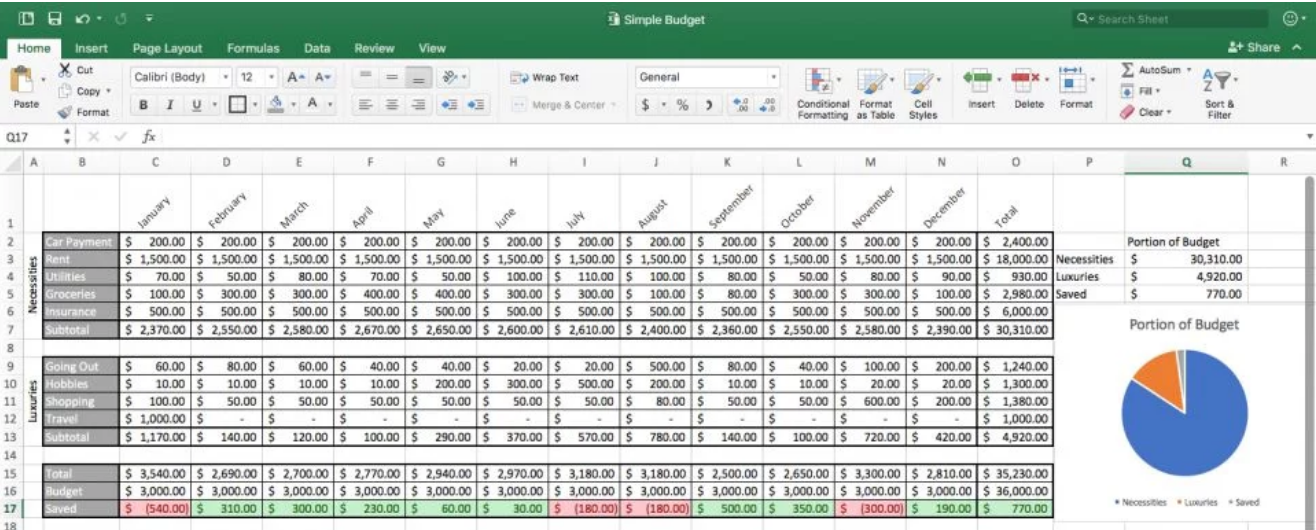
\includegraphics[width=0.7\linewidth]{img/excel-sheet-example}

This makes the analytical steps taken are not readily apparent, nor easy to reproduce. Have you ever done forensics on an Excel sheet, trying to understand what happened between columns or sheets? Maybe it was even your own Excel file from the (recent) past.

This also makes them pretty brittle/sensitive to minor changes. Has seeing this ever given you a feeling of horror:

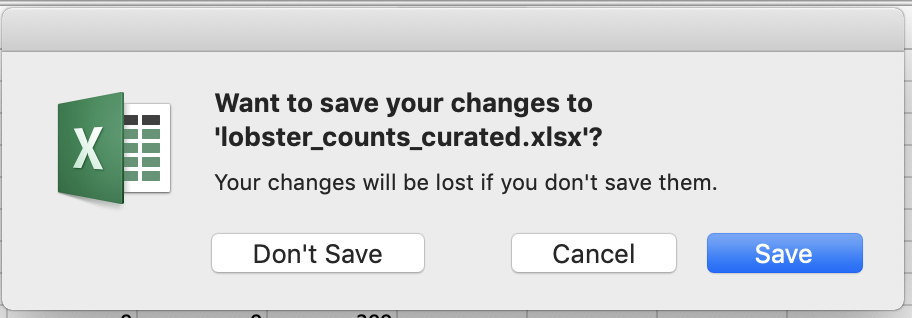
\includegraphics[width=0.8\linewidth]{img/want-to-save-changes-excel}

So while it is great how easily you can update different fields and add analytical steps in an Excel sheet, it can also be a bit hard to handle, particularly as projects get more complicated.

So, as automation, reproducibility, collaboration, and frequent reporting become increasingly expected in data analysis, a good option for Excel users is to extend their workflows with R.

\hypertarget{what-to-expect}{%
\subsection{What to expect}\label{what-to-expect}}

This is going to be a fun workshop.

This workshop will give you hands-on experience and confidence with R, and how to interoperate between Excel and R --- it is not about wholesale replacing everything you do in Excel into R.
We will learn technical skills that you can incrementally incorporate into your existing workflows. But a big part of interfacing between Excel and R is not only skillsets, it is mindsets. It is the mindset about how we think about data. How we shape data and organize data and analyze data. And how what we do now can make our analytical life better in the future.

\textbf{A modern R user has a workflow framed around collaboration}, and uses an ecosystem of tools and practices. We will be learning three main things all at the same time:

\begin{enumerate}
\def\labelenumi{\arabic{enumi}.}
\tightlist
\item
  coding with best practices (R/RStudio/tidyverse)
\item
  collaborative bookkeeping (Git/GitHub)
\item
  reporting and publishing (RMarkdown/GitHub)
\end{enumerate}

\textbf{R users keep raw data separate from their analyses}, which means having data in one file and written computational commands saved as a separate file. We also embrace the concept of \textbf{``tidy data''}, where the data has a rectangular shape and each column is a variable and each row is an observation. Tidy data is a way of life.

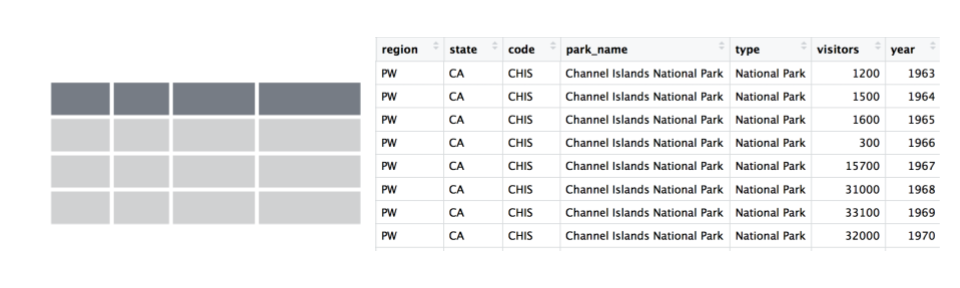
\includegraphics[width=0.7\linewidth]{img/tidy_img_np}

\textbf{We are going to go through a lot in these two days} and it's less important that you remember it all. More importantly, you'll have experience with it and confidence that you can do it. The main thing to take away is that there \emph{are} good ways to work between R and Excel; we will teach you to expect that so you can find what you need and use it! A theme throughout is that tools exist and are being developed by real, and extraordinarily nice, people to meet you where you are and help you do what you need to do.

\textbf{You are all welcome here}, please be respectful of one another. Everyone in this workshop is coming from a different place with different experiences and expectations. But everyone will learn something new here, because there is so much innovation in the data science world. Instructors and helpers learn something new every time, from each other and from your questions. If you are already familiar with some of this material, focus on how we teach, and how you might teach it to others. Use these workshop materials not only as a reference in the future but also for talking points so you can communicate the importance of these tools to your communities. A big part of this training is not only for you to learn these skills, but for you to also teach others and increase the value and practice of open data science in science as a whole.

\hypertarget{guiding-principles-recurring-themes}{%
\section{Guiding principles / recurring themes}\label{guiding-principles-recurring-themes}}

\textbf{``Keep the raw data raw''} --- A hard line separating raw data and analyses. In R, we have data in one file and written computational commands saved as a separate file.

\textbf{Scripted analyses} --- We write analytical logic in code (rather than clicks) so that can be understood, rerun, and built upon.

\textbf{Learn from data that are not your own} --- We aren't using your data in this workshop, but you will see similiarities and patterns, and you'll see that these tools and practices apply to your work.

\textbf{Think ahead for Future You, Future Us.} Help make lives easier --- first and foremost your own. Create breadcrumbs for yourselves and others: document and share your work.

\hypertarget{resources}{%
\section{Resources}\label{resources}}

R is not only a language, it is an active community of developers, users, and educators (often these traits are in each person). This workshop and book based on many excellent materials created by other members in the R community, who share their work freely to help others learn. Using community materials is how WE learned R, and each chapter of the book will have Resources listed for further reading into the topics we discuss. And, when there is no better way to explain something (ahem Jenny Bryan), we will quote or reference that work directly.

\begin{itemize}
\tightlist
\item
  \href{https://whattheyforgot.org/}{What They Forgot to Teach You About R} --- Jenny Bryan \& Jim Hester
\item
  \href{https://stat545.com/}{Stat545} --- Jenny Bryan \& Stat545 TAs
\item
  \href{http://rex-analytics.com/things-live-r-r-excel-users/}{Where do Things Live in R?} REX Analytics
\item
  \href{https://blog.shotwell.ca/posts/r_for_excel_users/}{}
\item
  \href{http://nssdeviations.com/episode-9-spreadsheet-drama}{Spreadsheet Drama (Episode 9)} --- Not So Standard Deviations with Roger Peng \& Hilary Parker
\item
  more to come!
\end{itemize}

\hypertarget{rstudio}{%
\chapter{R \& RStudio, RMarkdown}\label{rstudio}}

\hypertarget{summary}{%
\section{Summary}\label{summary}}

We'll learn RMarkdown, which helps you tell a story with your data analysis because you can write text alongside the code. We are actually learning two languages at once: R and Markdown.

\hypertarget{objectives}{%
\subsection{Objectives}\label{objectives}}

In this lesson we will:

\begin{itemize}
\tightlist
\item
  get oriented to the RStudio interface
\item
  explore RMarkdown.
\item
  discuss RMarkdown files vs Console (running vs knitting)
\item
  learn a few base R functions (\texttt{c()})
\item
  error messages and help pages
\item
  discuss and install packages (\texttt{here()}) usethis
\item
  intro pipe operator (\texttt{\%\textgreater{}\%})
\item
  configure Git (to prepare for next session)
\end{itemize}

\hypertarget{resources-1}{%
\subsection{Resources}\label{resources-1}}

\begin{itemize}
\tightlist
\item
  \href{https://blog.shotwell.ca/posts/r_for_excel_users/}{R for Excel Users} by Gordon Shotwell (blog)
\end{itemize}

\hypertarget{rstudio-orientation}{%
\section{RStudio Orientation}\label{rstudio-orientation}}

Open RStudio for the first time.

Launch RStudio/R.

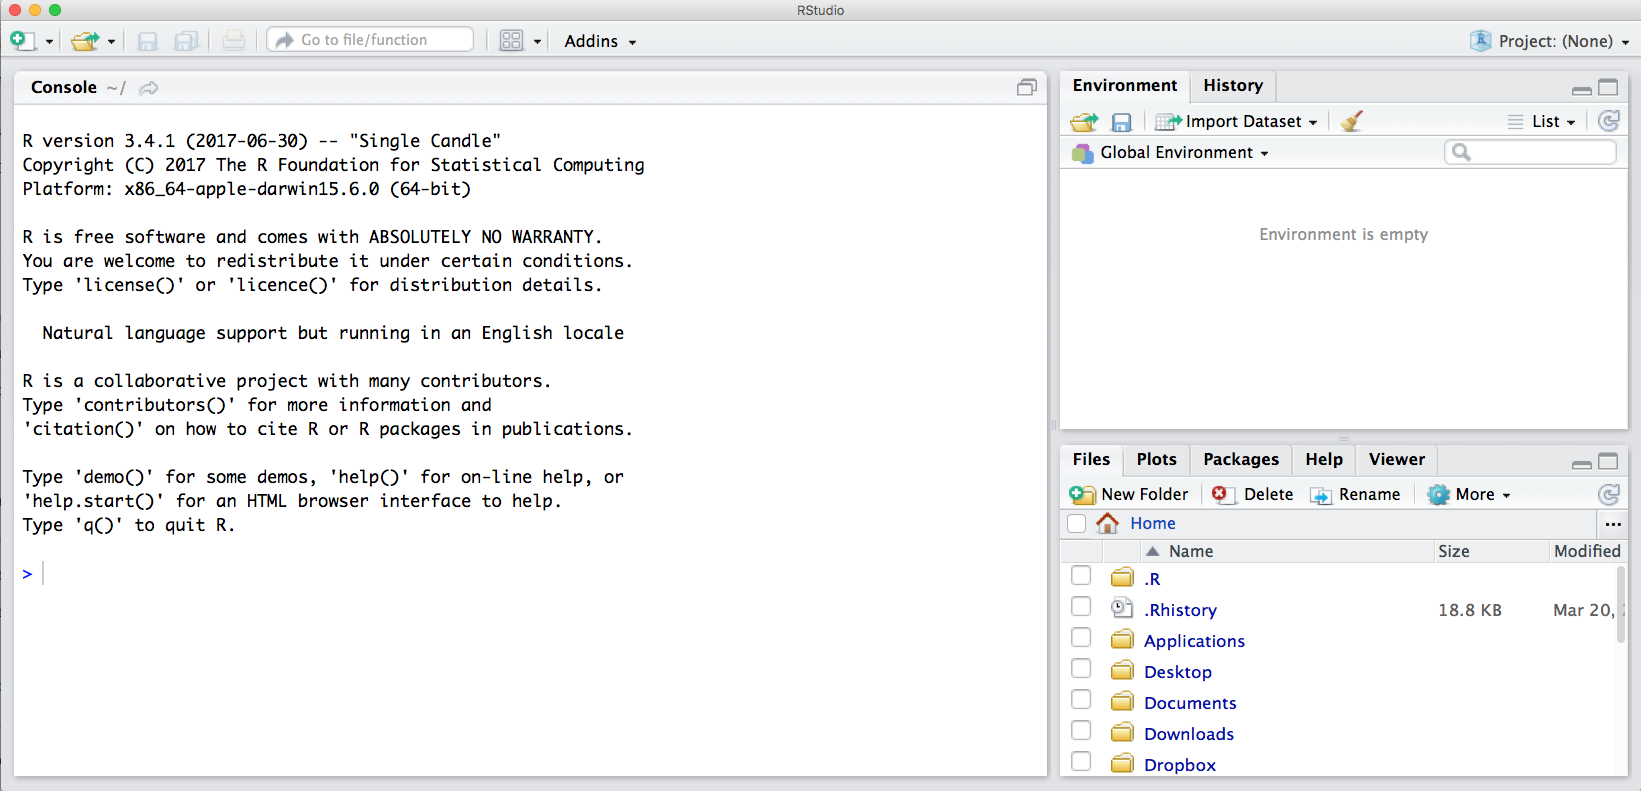
\includegraphics[width=0.8\linewidth]{img/RStudio_IDE}

Notice the default panes:

\begin{itemize}
\tightlist
\item
  Console (entire left)
\item
  Environment/History (tabbed in upper right)
\item
  Files/Plots/Packages/Help (tabbed in lower right)
\end{itemize}

We won't click through this all immediately but we will become familiar with more of the options and capabilities throughout the next few days.

Something critical to know now is that you can make everything you see BIGGER by going to the navigation pane: View \textgreater{} Zoom In. Learn these keyboard shortcuts; being able to see what you're typing will help avoid typos \& help us help you.

I think that \textbf{R is your airplane, and the RStudio IDE is your airport}. You are the pilot, and you use R to go places! With practice you'll gain skills and confidence; you can fly further distances and get through tricky situations. You will become an awesome pilot and can fly your plane anywhere. And the RStudio IDE provides support! Runways, communication, community, and other services that makes your life as a pilot much easier. It provides not only the infrastructure but a hub for the community that you can interact with.

An important first question: \textbf{where are we?}

If you've have opened RStudio for the first time, you'll be in your Home directory. This is noted by the \texttt{\textasciitilde{}/} at the top of the console. You can see too that the Files pane in the lower right shows what is in the Home directory where you are. You can navigate around within that Files pane and explore, but note that you won't change where you are: even as you click through you'll still be Home: \texttt{\textasciitilde{}/}.

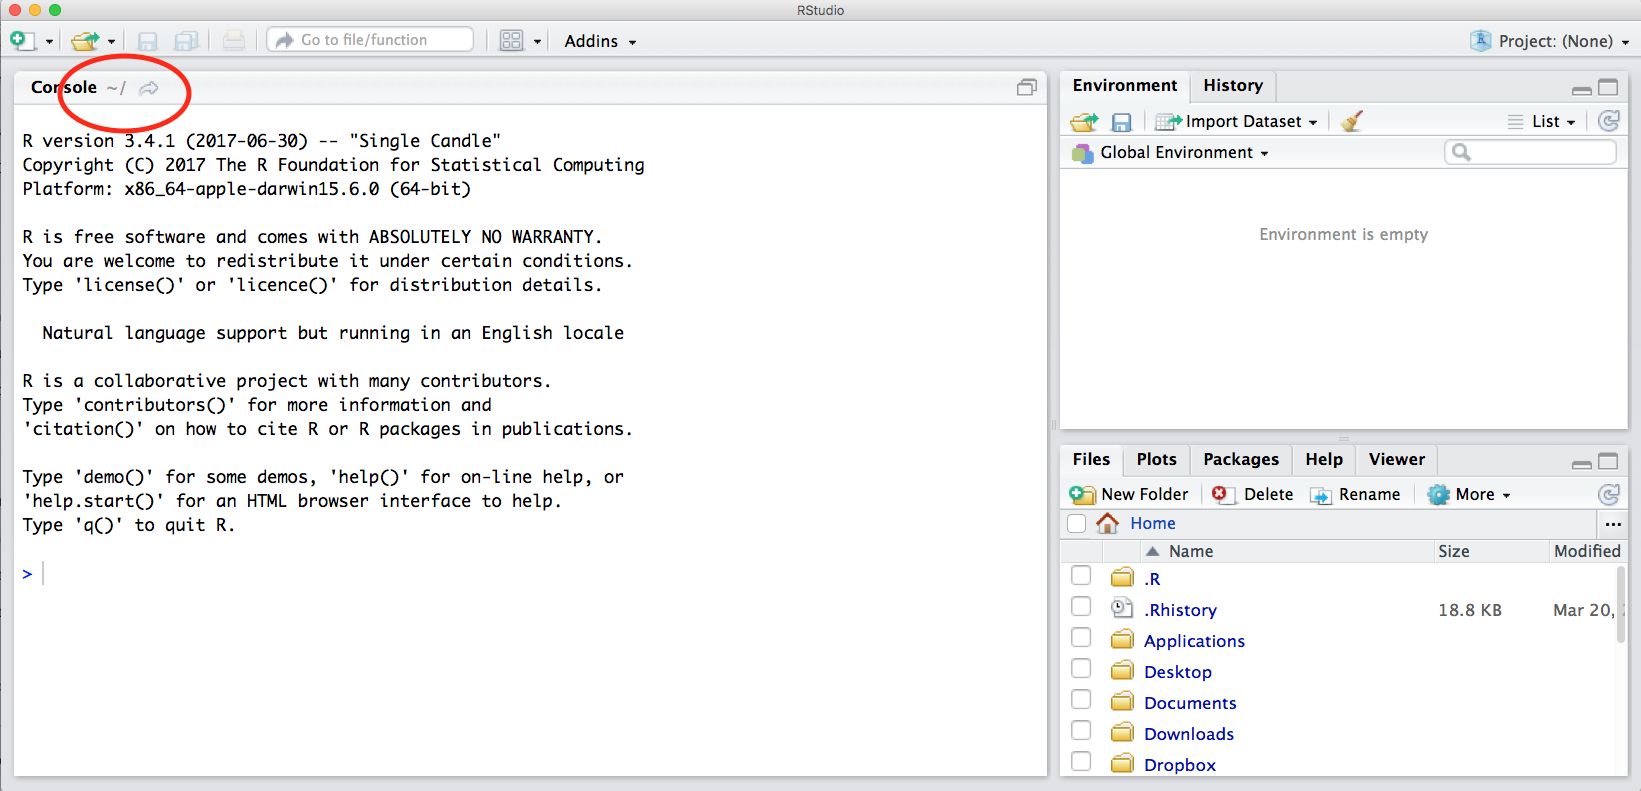
\includegraphics[width=0.8\linewidth]{img/RStudio_IDE_homedir}

We are going to have our first experience with R through RMarkdown, so let's do the following.

\hypertarget{intro-to-rmarkdown}{%
\section{Intro to RMarkdown}\label{intro-to-rmarkdown}}

An RMarkdown file is a plain text file that allow us to write code and text together, and when it is ``knit'', the code will be evaluated and the text formatted so that it creates a reproducible report or document that is nice to read as a human.

This is really critical to reproducibility, and it also saves time. This document will recreate your figures for you in the same document where you are writing text. So no more doing analysis, saving a plot, pasting that plot into Word, redoing the analysis, re-saving, re-pasting, etc.

Let's experience this a bit ourselves and then we'll talk about it more.

\hypertarget{create-an-rmarkdown-file}{%
\subsection{Create an RMarkdown file}\label{create-an-rmarkdown-file}}

Let's do this together:

File -\textgreater{} New File -\textgreater{} RMarkdown\ldots{} (or alternatively you can click the green plus in the top left -\textgreater{} RMarkdown).

Let's title it ``Testing'' and write our name as author, then click OK with the recommended Default Output Format, which is HTML.

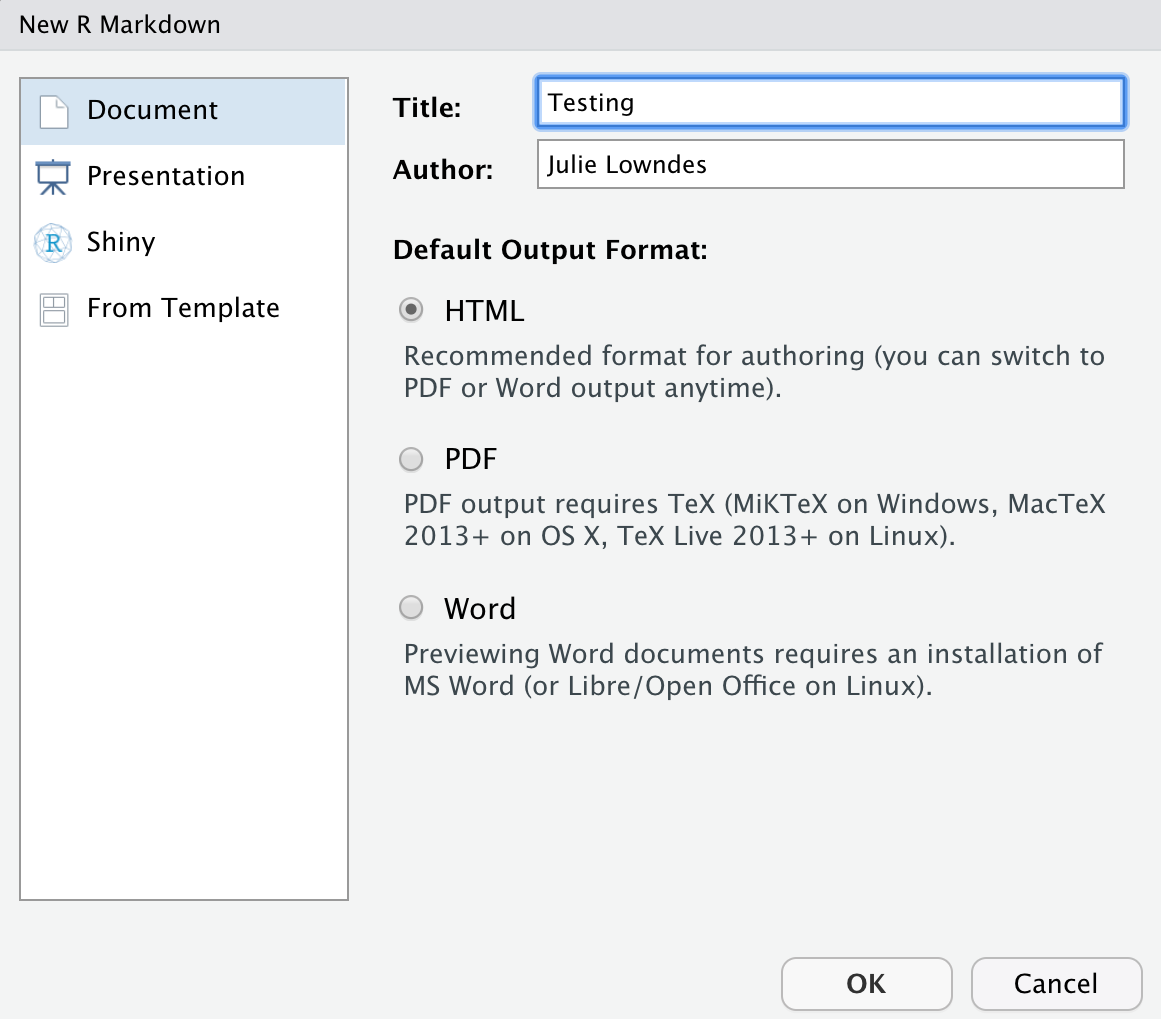
\includegraphics[width=0.8\linewidth]{img/rstudio_new-rmd-doc-html}

OK, first off: by opening a file, we are seeing the 4th pane of the RStudio console, which is essentially a text editor. This lets us organize our files within RStudio instead of having a bunch of different windows open.

Let's have a look at this file --- it's not blank; there is some initial text is already provided for you. Let's have a high-level look through of it:

\begin{itemize}
\tightlist
\item
  The top part has the Title and Author we provided, as well as today's date and the output type as an HTML document like we selected above.
\item
  There are white and grey sections. These are the 2 main languages that make up an RMarkdown file.

  \begin{itemize}
  \tightlist
  \item
    \textbf{Grey sections are R code}
  \item
    \textbf{White sections are Markdown text}
  \end{itemize}
\item
  There is black and blue text.
\end{itemize}

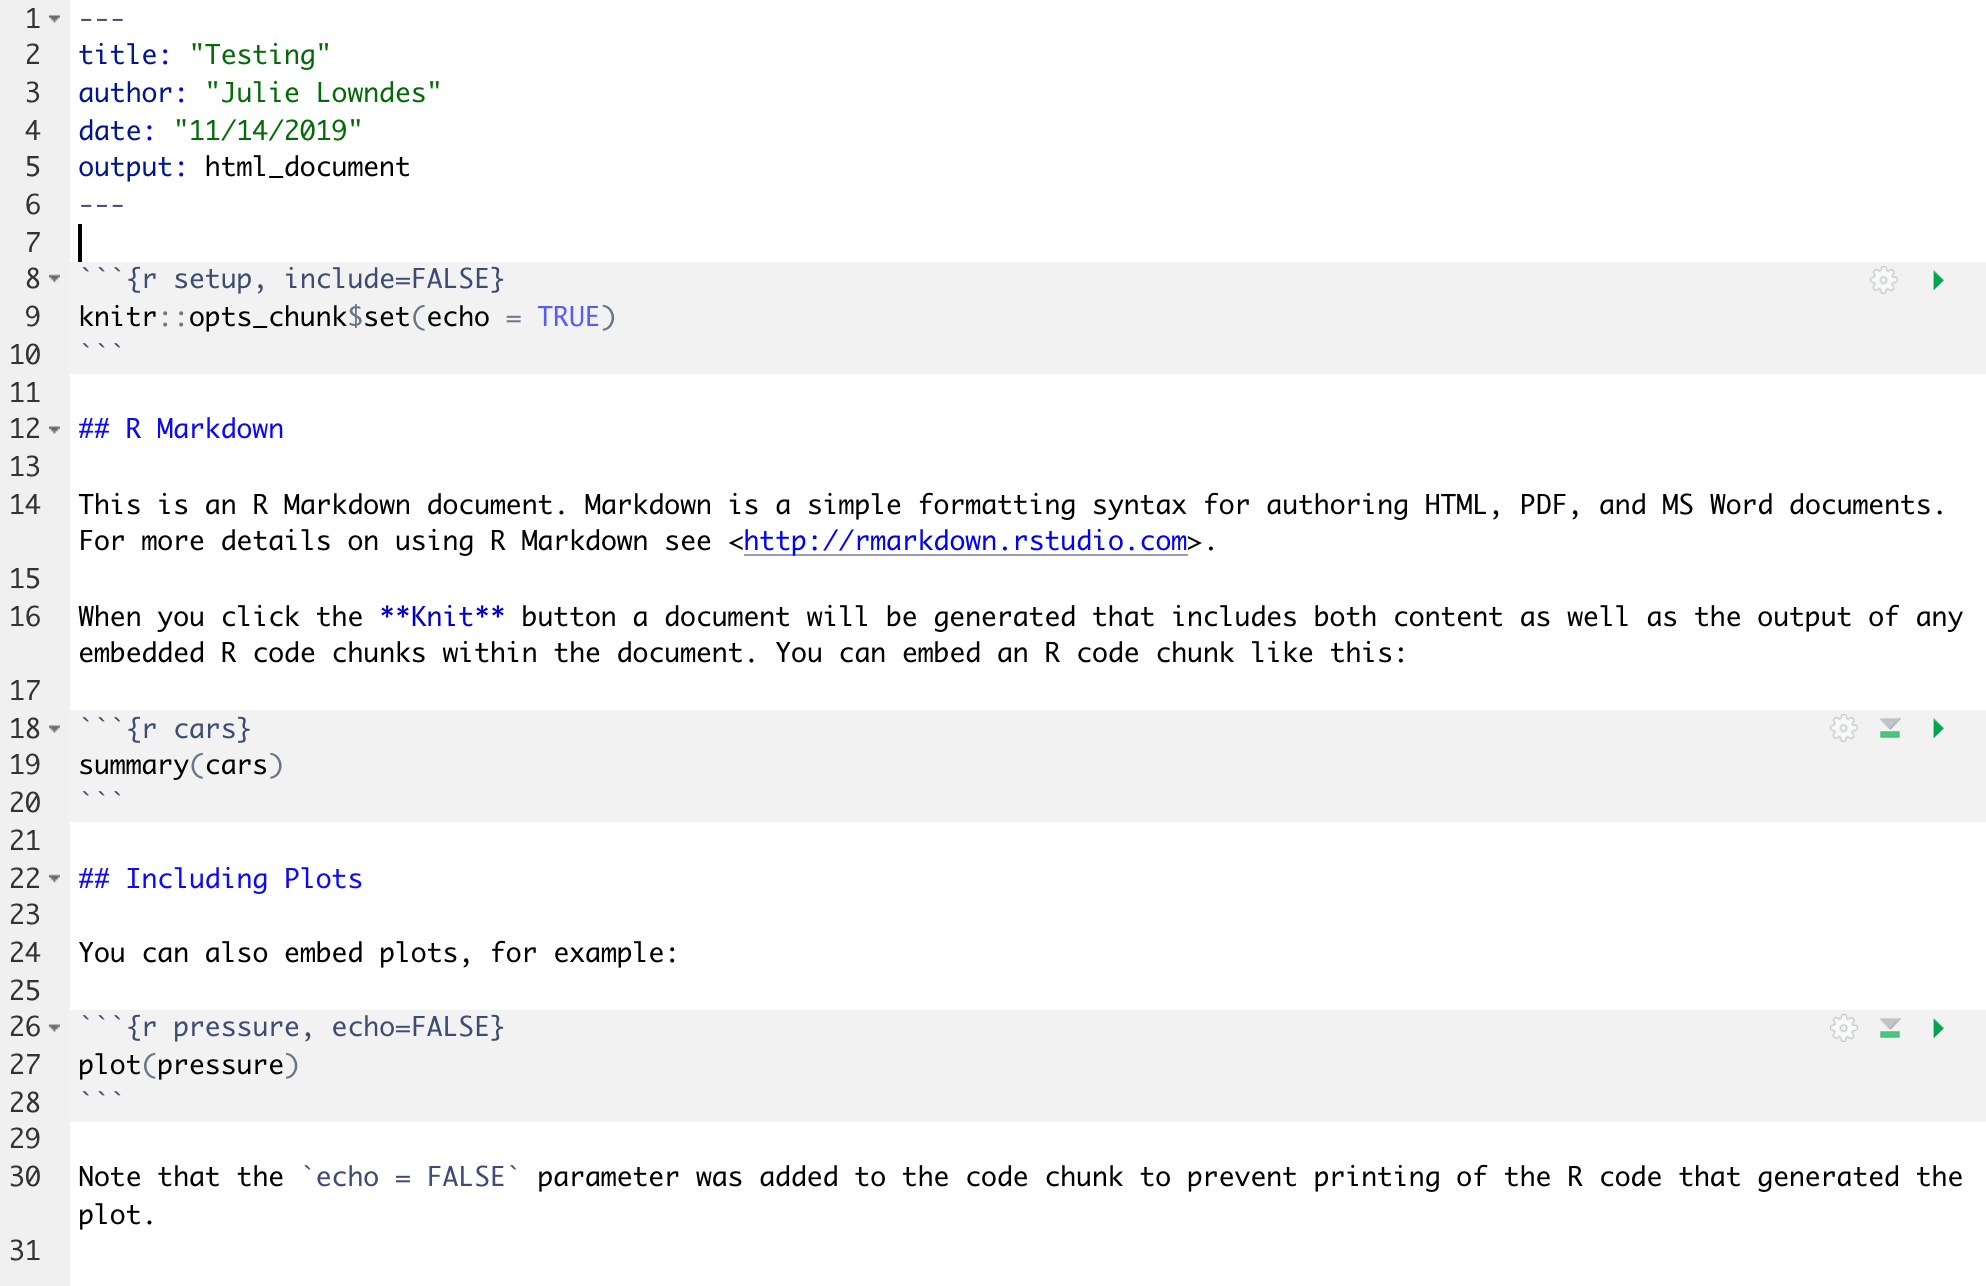
\includegraphics[width=0.8\linewidth]{img/rmarkdown}

\hypertarget{knit-your-rmarkdown-file}{%
\subsection{Knit your RMarkdown file}\label{knit-your-rmarkdown-file}}

Let's go ahead and ``Knit'' by clicking the blue yarn at the top of the RMarkdown file.
It's going to ask us to save first, I'll name mine ``testing.Rmd''. Note that this is by default going to save this file in your home directory \texttt{/\textasciitilde{}}. Since this is a testing document this is fine to save here; we will get more organized about where we save files very soon. Once you click Save, the knit process will be able to continue.

OK so how cool is this, we've just made an html file! This is a single webpage that we are viewing locally on our own computers. Knitting this RMarkdown document has rendered --- we also say formatted --- both the Markdown text (white) and the R code (grey), and the it also executed --- we also say ran --- the R code.

Let's have a look at them side-by-side:

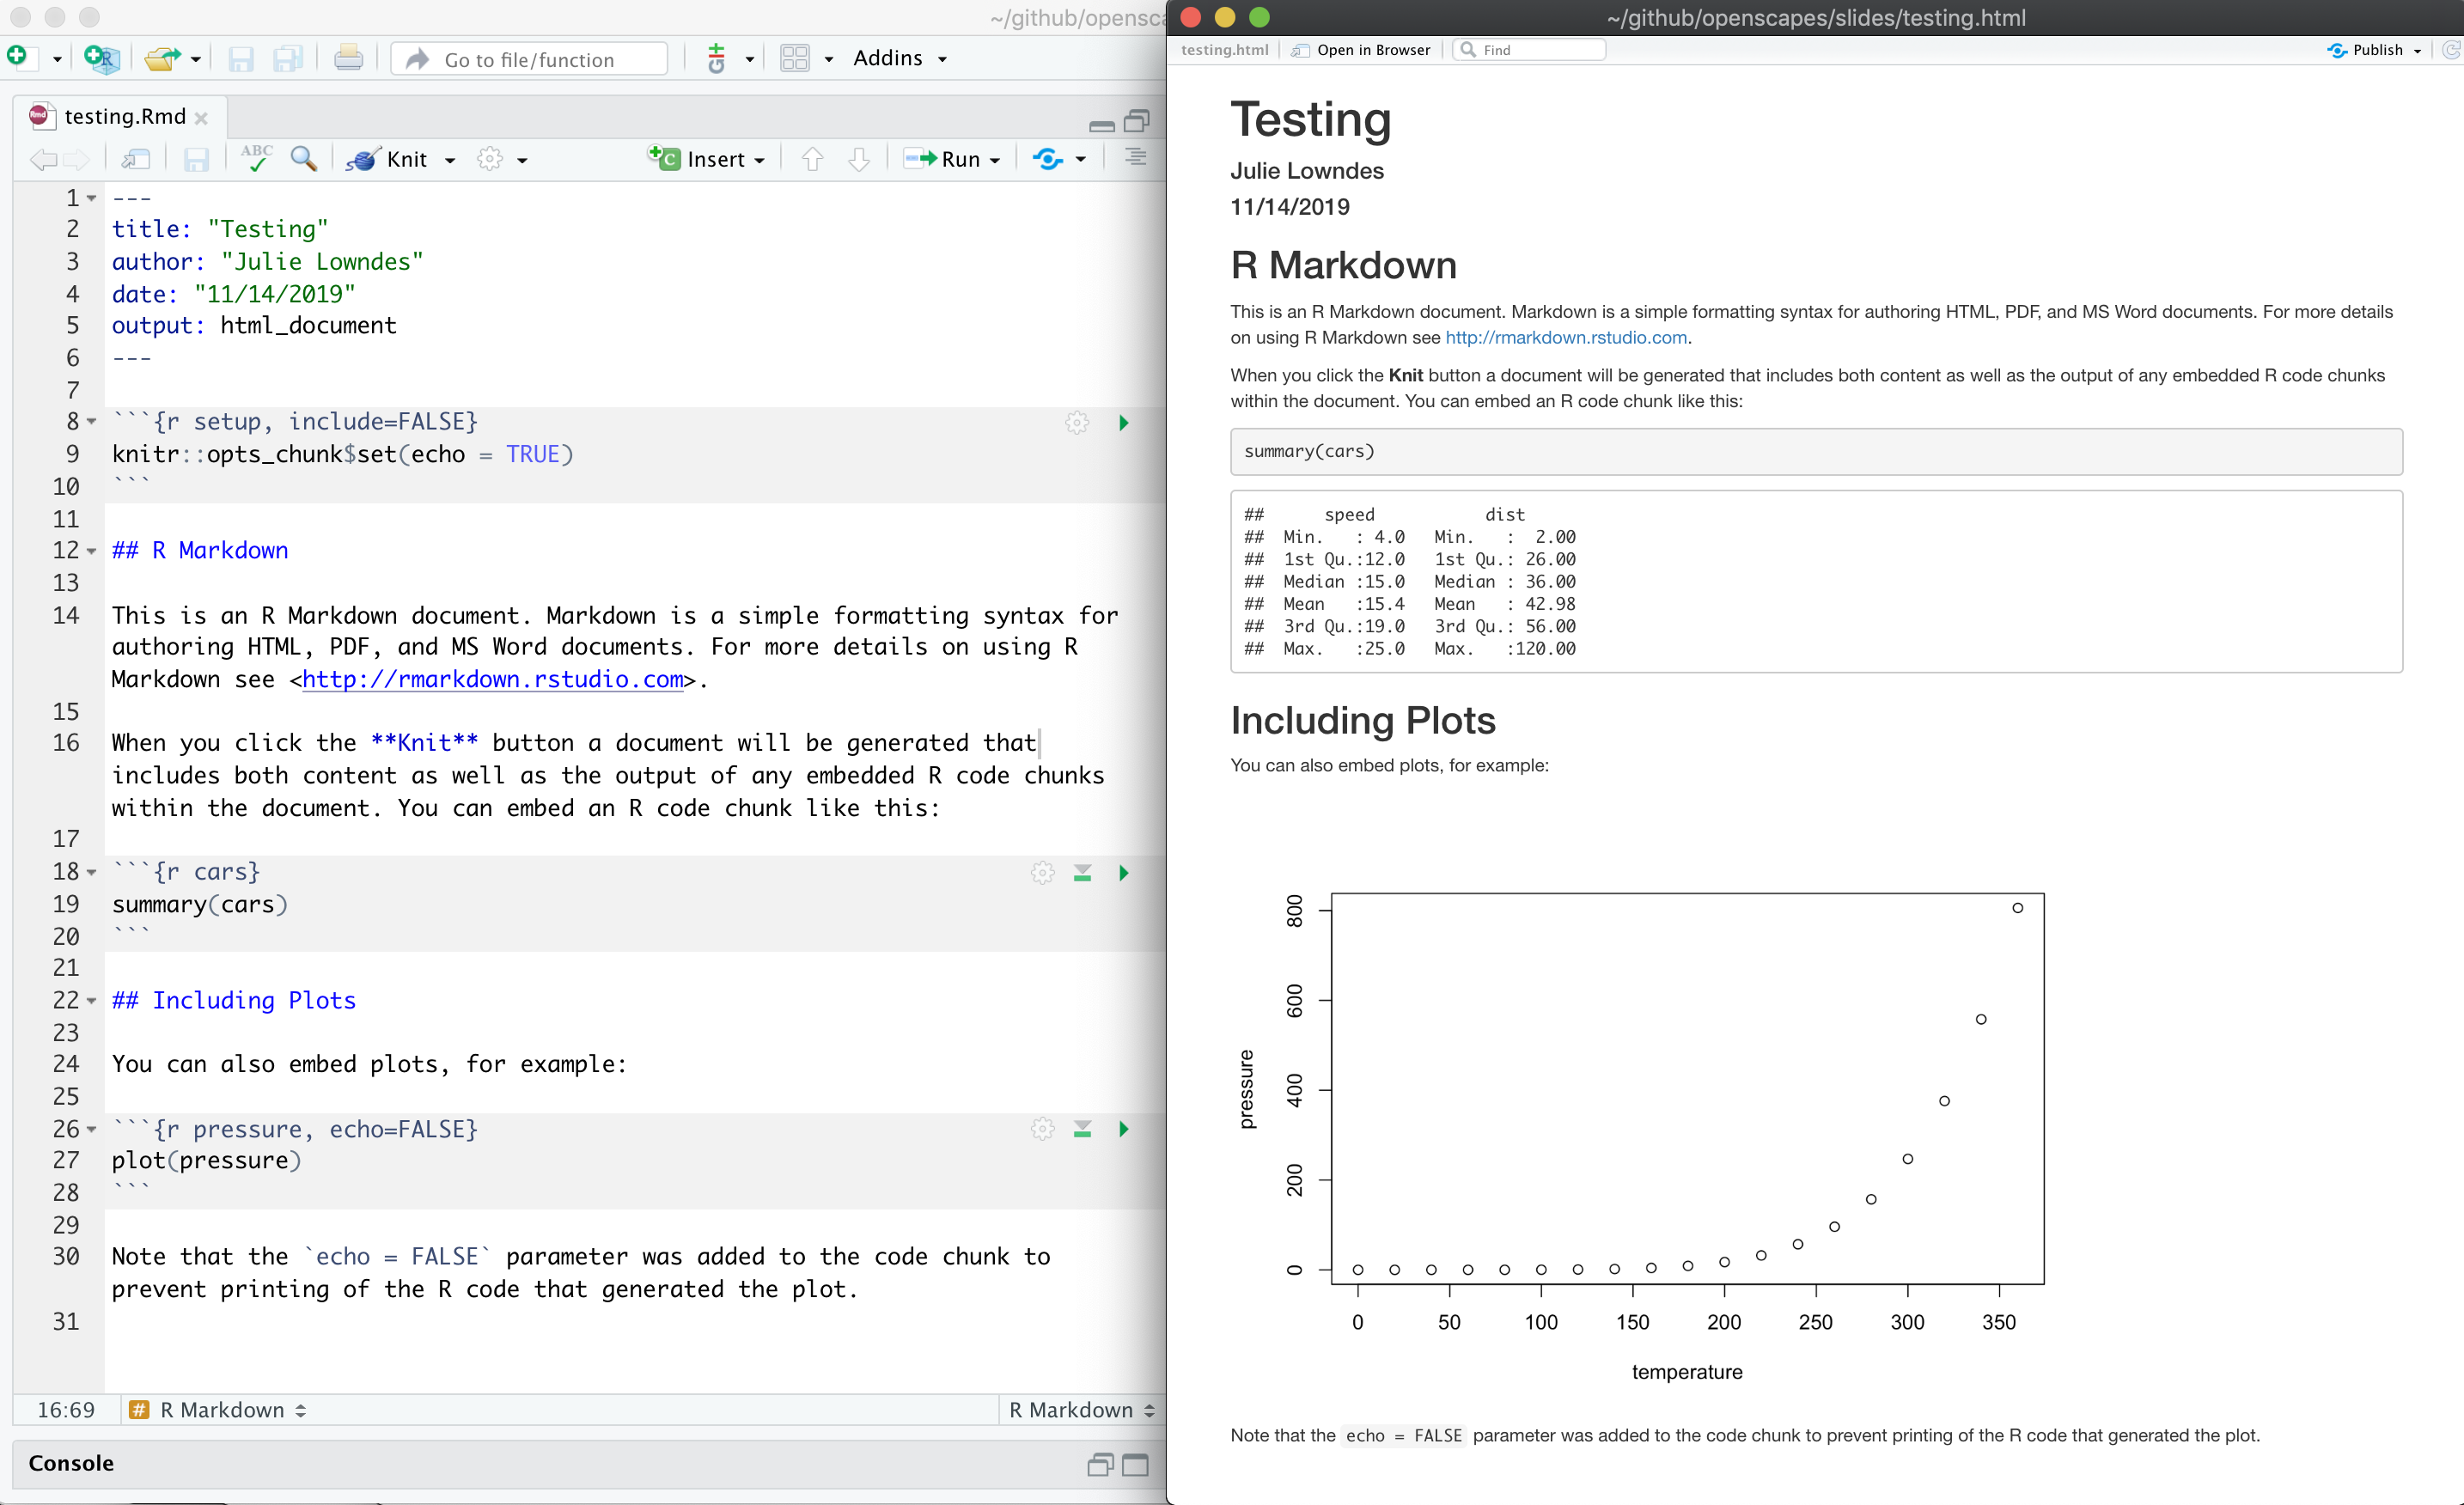
\includegraphics[width=0.8\linewidth]{img/rmarkdown_side_by_side}

Let's take a deeper look at these two files. So much of learning to code is looking for patterns.

\hypertarget{markdown-text}{%
\subsection{Markdown text}\label{markdown-text}}

To warm us up for R, let's start by talking about another language, Markdown. This is a formatting language for plain text, and there are only about 15 rules to know.

Notice the syntax for:

\begin{itemize}
\tightlist
\item
  \textbf{headers} get rendered at multiple levels: \texttt{\#}, \texttt{\#\#}
\item
  \textbf{bold}: \texttt{**word**}
\end{itemize}

There are some good \href{https://github.com/adam-p/markdown-here/wiki/Markdown-Here-Cheatsheet}{cheatsheets} to get you started, and here is one built into RStudio: Go to Help \textgreater{} Markdown Quick Reference

\hypertarget{r-code}{%
\subsection{R code}\label{r-code}}

Let's look at the R code that we see executed in our knitted document.

We see that \texttt{summary(cars)} produces a table

And we see that \texttt{plot(pressure)} produces a plot.

\texttt{cars} and \texttt{pressure} are small datasets that come with R out-of-the-box.

\hypertarget{code-chunks}{%
\subsection{Code chunks}\label{code-chunks}}

Let's start of by looking at the 3 code chunks, which are grey.

Each of them are start by 3 backticks and \texttt{\{r\ label\}}, which signify that there will be R code inside, and they are each given a unique name. Anything inside the brackets (\texttt{\{\ \}}) is instructions for RMarkdown about that code to run. For example:

\begin{itemize}
\tightlist
\item
  the first chunk says \texttt{include=FALSE}, and we don't see it included in the HTML document.
\item
  the second chunk has no additional instructions, and in the HTML document we see the code and the evaluation of that code (a summary table)
\item
  the third chunk says \texttt{echo=FALSE}, and in the HTML document we do not see the code echoed, we only see the plot when the code is executed.
\end{itemize}

There are many more options available and we will explore more as we go.

\hypertarget{naming-code-chunks-deep-thought}{%
\subsubsection{Naming code chunks (Deep thought?)}\label{naming-code-chunks-deep-thought}}

All three chunks say \texttt{r} as the language, and have a label (\texttt{setup}, \texttt{cars}, \texttt{pressure}. This is to help us navigate between them and keep them organized. They are optional, but will become powerful as you become a powerful R user. But if you label your code chunks, you must have unique labels. Otherwise you will see an error when you try to knit:

\begin{verbatim}
processing file: Untitled.Rmd
Error in parse_block(g[-1], g[1], params.src) : duplicate label 'cars'
Calls: <Anonymous> ... process_file -> split_file -> lapply -> FUN -> parse_block
Execution halted
\end{verbatim}

In this case, you read the error message. Not everything immediately looks like something I would know anything about, but pressing on still allows me to identify the problem: ``duplicate label `cars'\,''.

\hypertarget{delete-everything-and-reknit}{%
\subsubsection{Delete everything and reknit}\label{delete-everything-and-reknit}}

R knows that a file with extension .Rmd is a special file to be knit. But it does not rely on any of this stuff that is in the template file.

Do this: delete all the content from this file. You can do this by dragging your cursor to highlight all text, or use the keyboard shortcut Command-A. And then delete. You should now have a blank document.

To demo that it will still knit, let's write \texttt{\#\ Julie\textquotesingle{}s\ workshop\ notes} (with your name) and reknit.

This will be your notes.

The reason we use RMarkdown or an R script is so that we can write down our code once in our script but then can execute it as many times as we want.

\hypertarget{new-code-chunks}{%
\subsubsection{New code chunks}\label{new-code-chunks}}

We can create a new chunk in your RMarkdown first in one of these ways:

\begin{itemize}
\tightlist
\item
  click ``Insert \textgreater{} R'' at the top of the editor pane
\item
  type by hand
  ```\{r\}
  ```
\item
  if you haven't deleted a chunk that came with the new file, edit that one
\end{itemize}

\begin{quote}
Cool tip: doesn't have to be only R, other languages supported.
\end{quote}

Now, let's write some code in R. Let's say we want to plot the cars data. I'm going to press enter to to add some extra carriage returns because sometimes I find it easier to look at my code when there is a bit more space, and R lets you use as much whitespace as you would like.

\begin{Shaded}
\begin{Highlighting}[]
\KeywordTok{plot}\NormalTok{(cars)}
\end{Highlighting}
\end{Shaded}

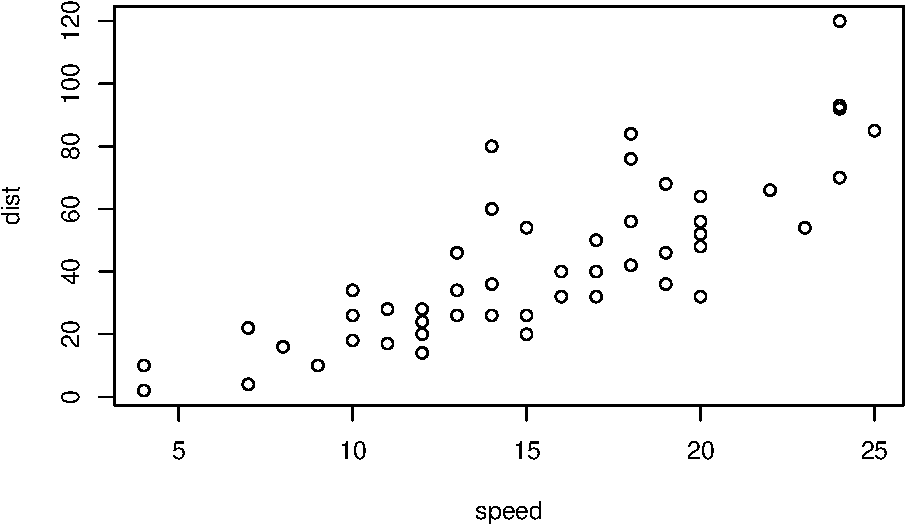
\includegraphics{R-for-Excel-Users_files/figure-latex/unnamed-chunk-10-1.pdf}

We can knit this and see the plot of cars. This is the same data that we made the summary table with.

\begin{quote}
Troubleshooting: If you could not successfully knit your document without error, Look at your code again. Do you have both open \texttt{(} and close \texttt{)} parentheses? Are your code chunk fences correct?
\end{quote}

\hypertarget{running-r-code}{%
\subsection{Running R code}\label{running-r-code}}

Knitting the document is great, and you can see all your updates rendered nicely. But you can imagine that this would be tedious that if every time you made an update you needed to knit this document. We can run R code in the Console.

TODO: build out more about Console

To run, we need to get what we typed in the the R chunk (the grey R code) down into the console. How do we do it? There are several ways (let's do each of them):

\begin{enumerate}
\def\labelenumi{\arabic{enumi}.}
\tightlist
\item
  copy-paste this line into the console.
\item
  select the line (or simply put the cursor there), and click `Run'. This is available from

  \begin{enumerate}
  \def\labelenumii{\alph{enumii}.}
  \tightlist
  \item
    the bar above the file (green arrow)
  \item
    the menu bar: Code \textgreater{} Run Selected Line(s)
  \item
    keyboard shortcut: command-return
  \end{enumerate}
\item
  click the green arrow at the right of the code chunk
\end{enumerate}

\begin{quote}
Troubleshooting: The following error is because you also highlighted and asked to run ```\texttt{\{r\}}, and this is the code fencing, not R code itself.
\end{quote}

\begin{verbatim}
Error: attempt to use zero-length variable name
\end{verbatim}

What is \texttt{plot} anyways? It is a function. Let's talk about that next.

\hypertarget{r-functions}{%
\section{R Functions}\label{r-functions}}

TODO --- add c()?

Like Excel, some of the biggest power in R is that there are built-in functions that you can use in your analyses (and, as we'll see, R users can easily create and share functions, and it is this open source developer and contributor community that makes R so awesome).

R has a mind-blowing collection of built-in functions that are used with the same syntax: function name with parentheses around what the function needs to do what it is supposed to do.

TODO: swap out for simpler

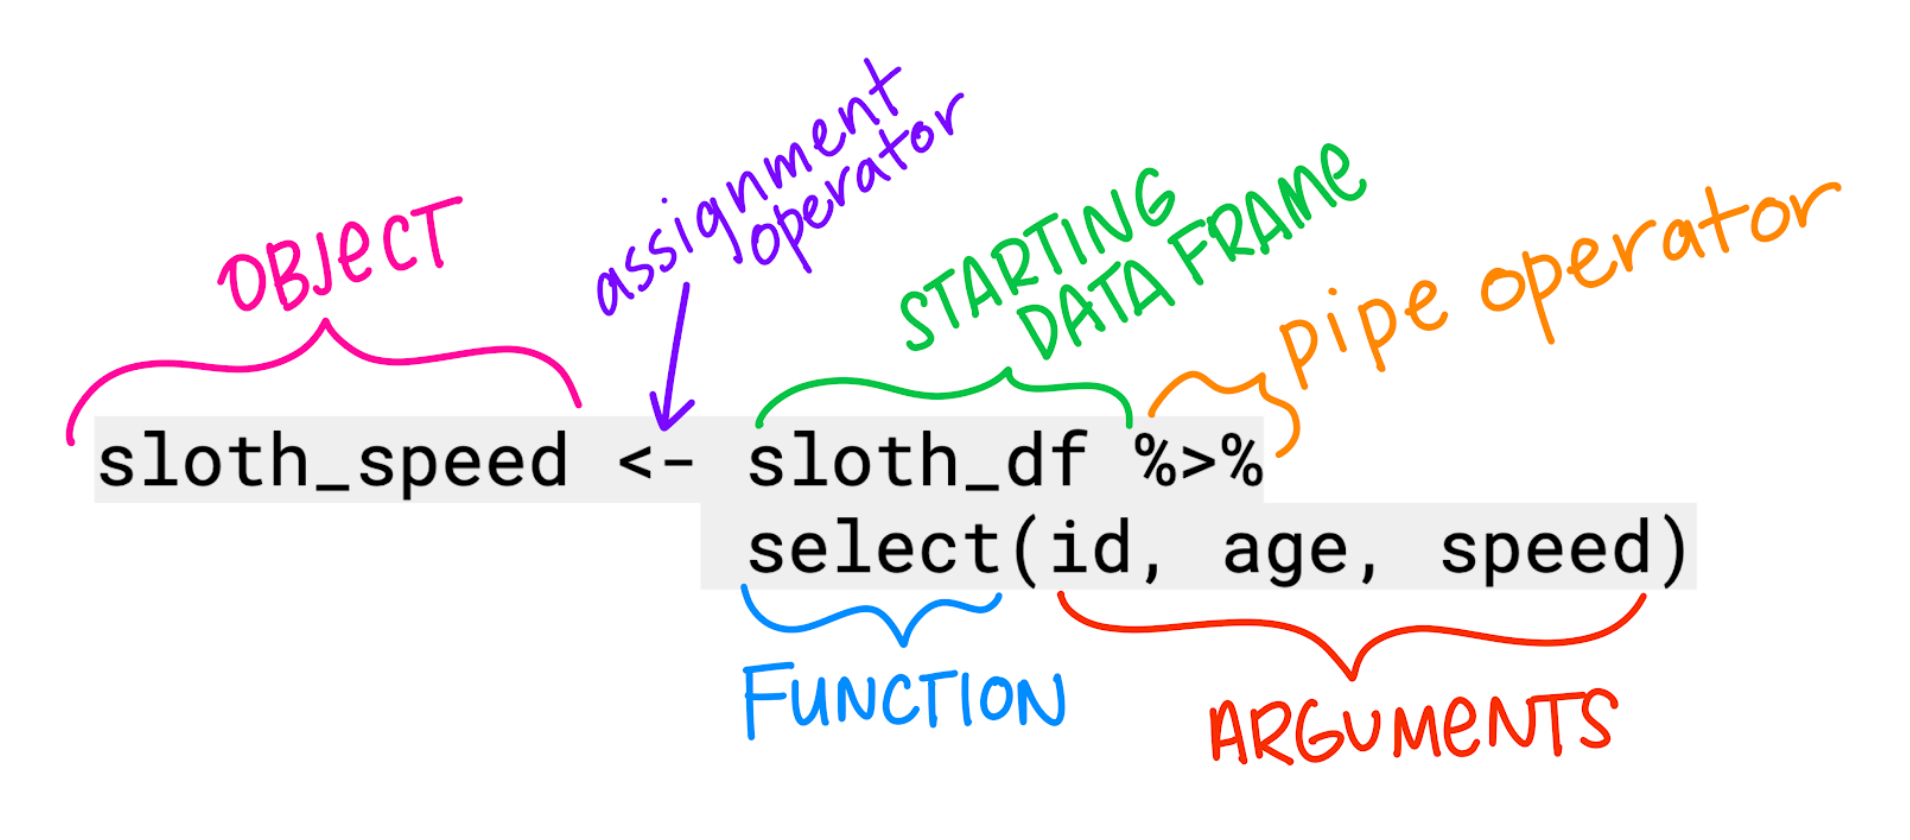
\includegraphics[width=0.6\linewidth]{img/horst-naming-terms}

\texttt{function\_name(argument1\ =\ value1,\ argument2\ =\ value2,\ ...)}. When you see this syntax, we say we are ``calling the function''.

So with \texttt{plot()}, the arguments it requires are \texttt{x} and \texttt{y}, and when we pass \texttt{cars} to plot(), R is able to understand that it should use the two columns in that dataset as x and y.

\hypertarget{help-pages}{%
\section{Help pages}\label{help-pages}}

\emph{TODO - complete}

A good way to learn about functions is to look at the help pages. Let's navigate over to the Help tab and type \texttt{plot}. All help pages will have the same format, here is how I look at it:

The help page tells the name of the package in the top left, and broken down into sections:

\begin{itemize}
\tightlist
\item
  Description: An extended description of what the function does.
\item
  Usage: The arguments of the function and their default values.
\item
  Arguments: An explanation of the data each argument is expecting.
\item
  Details: Any important details to be aware of.
\item
  Value: The data the function returns.
\item
  See Also: Any related functions you might find useful.
\item
  Examples: Some examples for how to use the function.
\end{itemize}

When I look at a help page, I start with the description, which might be too in-the-weeds for the level of understanding I need at the offset. For the \texttt{sum} page, it is pretty straight-forward and lets me know that yup, this is the function I want.

I next look at the usage and arguments, which give me a more concrete view into what the function does. This syntax looks a bit cryptic but what it means is that you use it by writing sum, and then passing whatever you want to it in terms of data: that is what the ``\ldots{}'' means. And the ``na.rm=FALSE'' means that by default, it will not remove NAs (I read this as: ``remove NAs? FALSE!'')

Then, I usually scroll down to the bottom to the examples. This is where I can actually see how the function is used, and I can also paste those examples into the Console to see their output. Let's try it:

\begin{Shaded}
\begin{Highlighting}[]
\KeywordTok{plot}\NormalTok{(sin, }\OperatorTok{-}\NormalTok{pi, }\DecValTok{2}\OperatorTok{*}\NormalTok{pi)}
\end{Highlighting}
\end{Shaded}

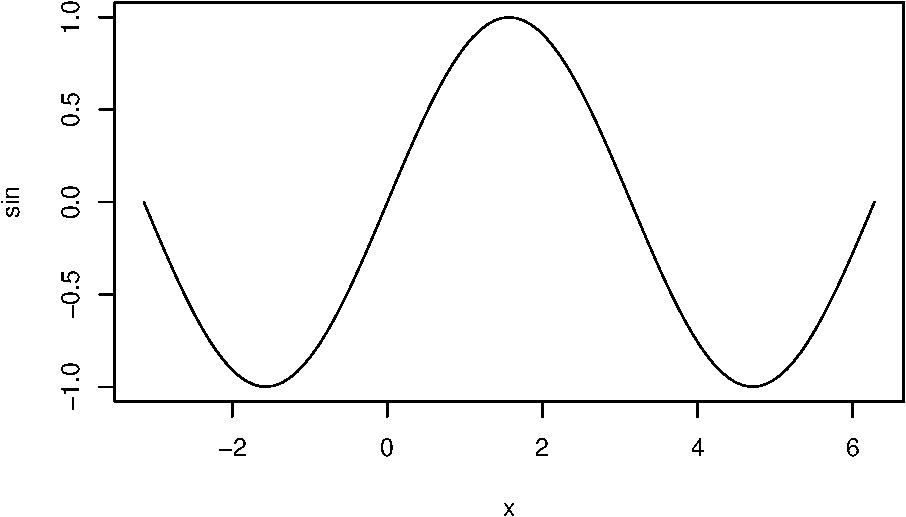
\includegraphics{R-for-Excel-Users_files/figure-latex/plot-help-example-1.pdf}

Let's try another function. In Excel, there is a ``SUM'' function to calculate a total. Let's expect that there is the same in R. I will type this into the Console:

\begin{Shaded}
\begin{Highlighting}[]
\KeywordTok{sum}\NormalTok{(}\DecValTok{1}\NormalTok{, }\DecValTok{2}\NormalTok{, }\DecValTok{3}\NormalTok{)}
\end{Highlighting}
\end{Shaded}

R is case-sensitive. So ``sum'' is a completely different thing to ``Sum'' or ``SUM''. And this is true for the names of functions, data sets, variable names, and data itself (``blue'' vs ``Blue'').

Awesome. Let's try this on our \texttt{cars} data

\begin{Shaded}
\begin{Highlighting}[]
\KeywordTok{sum}\NormalTok{(cars)}
\end{Highlighting}
\end{Shaded}

Alright. What is this number? It is the sum of ALL of the data in the \texttt{cars} dataset. Maybe in some analysis this would be a useful operation, but I would worry about the way your data is set up and your analyses if this is ever something you'd want to do. More likely, you'd want to take the sum of a specific column. In R, you can do that with the \texttt{\$} operator.

Let's say we want to calculate the total distance:

\begin{Shaded}
\begin{Highlighting}[]
\KeywordTok{sum}\NormalTok{(cars}\OperatorTok{$}\NormalTok{dist)}
\end{Highlighting}
\end{Shaded}

Let's do one more: try using \texttt{c()} which combines values together.

So let's create a new R code chunk. And we'll write:

\begin{Shaded}
\begin{Highlighting}[]
\KeywordTok{c}\NormalTok{(}\DecValTok{1}\NormalTok{, }\DecValTok{7}\OperatorTok{:}\DecValTok{9}\NormalTok{)}
\end{Highlighting}
\end{Shaded}

\begin{verbatim}
## [1] 1 7 8 9
\end{verbatim}

So you can see that this combines these values all into the same place, which is called a vector here. But let's learn more about what this does.

Let's do one more. Not all functions have (or require) arguments:

\begin{Shaded}
\begin{Highlighting}[]
\KeywordTok{date}\NormalTok{()}
\end{Highlighting}
\end{Shaded}

\begin{verbatim}
## [1] "Thu Jan  9 09:21:09 2020"
\end{verbatim}

Let's try combining some of these things together.

\begin{Shaded}
\begin{Highlighting}[]
\KeywordTok{c}\NormalTok{(}\StringTok{"R is awesome"}\NormalTok{, }\KeywordTok{date}\NormalTok{())}
\end{Highlighting}
\end{Shaded}

\begin{verbatim}
## [1] "R is awesome"             "Thu Jan  9 09:21:09 2020"
\end{verbatim}

We can also save this as an object.

\hypertarget{assigning-objects-with--}{%
\section{\texorpdfstring{Assigning objects with \texttt{\textless{}-}}{Assigning objects with \textless{}-}}\label{assigning-objects-with--}}

TODO refine

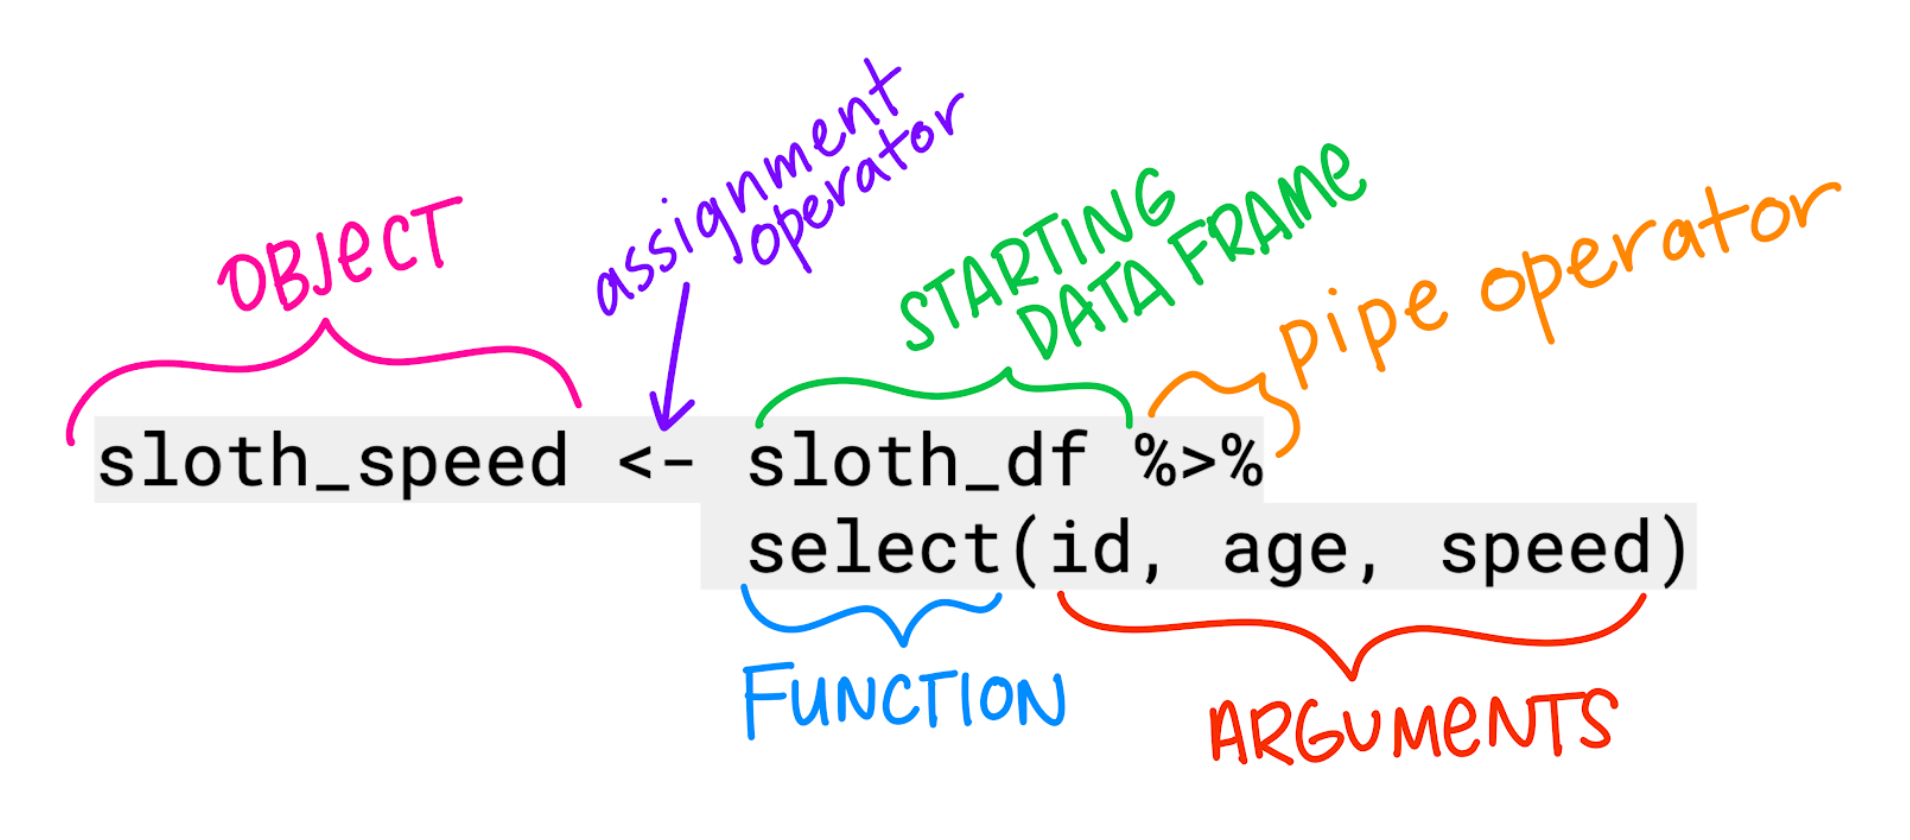
\includegraphics[width=0.6\linewidth]{img/horst-naming-terms}

This might be a really important thing that we want to be able to work with later. We can save this as its own object.

\begin{Shaded}
\begin{Highlighting}[]
\NormalTok{my_object <-}\StringTok{ }\KeywordTok{c}\NormalTok{(}\StringTok{"R is awesome"}\NormalTok{, }\KeywordTok{date}\NormalTok{())}
\end{Highlighting}
\end{Shaded}

This is a big difference with Excel, where you usually identify data by its location on the grid, like \texttt{\$A1:D\$20}. (You can do this with Excel by naming ranges of cells, but many people don't do this.)

Data can be a variety of formats, like numeric and text.

We do this by writing the name along with the assignment operator \texttt{\textless{}-}

\begin{Shaded}
\begin{Highlighting}[]
\NormalTok{sum_dist <-}\StringTok{ }\KeywordTok{sum}\NormalTok{(cars}\OperatorTok{$}\NormalTok{dist)}
\end{Highlighting}
\end{Shaded}

And we can execute it. In my head I hear ``sum\_dist gets 2149''.

Object names can be whatever you want, although they cannot start with a digit and cannot contain certain other characters such as a comma or a space. Different folks have different conventions; you will be wise to adopt a \href{http://en.wikipedia.org/wiki/Snake_case}{convention for demarcating words} in names.

\begin{Shaded}
\begin{Highlighting}[]
\CommentTok{# i_use_snake_case}
\CommentTok{# other.people.use.periods}
\CommentTok{# evenOthersUseCamelCase}
\end{Highlighting}
\end{Shaded}

\hypertarget{console-vs.rmarkdownr-script}{%
\section{Console vs.~RMarkdown/R script}\label{console-vs.rmarkdownr-script}}

\hypertarget{r-code-in-the-console}{%
\section{R code in the Console}\label{r-code-in-the-console}}

There is another way to get to the help pages besides clicking on the Help tab --- we can write this in R with \texttt{?}.

Let's try this with\ldots{}c()?

Every time we run R code, it is sent to the Console.

\hypertarget{r-packages}{%
\section{R Packages}\label{r-packages}}

TODO: update, with here()

So far we've been using a couple functions from base R, such as \texttt{sum()} and \texttt{plot()}. But, one of the amazing things about R is that a vast user community is always creating new functions and packages that expand R's capabilities. In R, the fundamental unit of shareable code is the package. A package bundles together code, data, documentation, and tests, and is easy to share with others. They increase the power of R by improving existing base R functionalities, or by adding new ones.

The traditional place to download packages is from CRAN, the \href{https://cran.r-project.org/}{Comprehensive R Archive Network}, which is where you downloaded R. CRAN is like a grocery store for vetted R packages.

You can also install packages from GitHub, which we'll do tomorrow.

You don't need to go to CRAN's website to install packages, this can be accomplished within R using the command \texttt{install.packages("package-name-in-quotes")}. Let's install our first package \texttt{here}. You need to use quotes around the package name.

Do this in the Console instead of in your RMarkdown file because we don't want this to load every time:

\begin{Shaded}
\begin{Highlighting}[]
\KeywordTok{install.packages}\NormalTok{(}\StringTok{"here"}\NormalTok{)}
\end{Highlighting}
\end{Shaded}

Now we've installed the package, but we need to tell R that we are going to use the functions within the \texttt{praise} package. We do this by using the function \texttt{library()}.

In my mind, this is analogous to needing to wire your house for electricity: this is something you do once; this is \texttt{install.packages}. But then you need to turn on the lights each time you need them (R Session).

\begin{Shaded}
\begin{Highlighting}[]
\KeywordTok{library}\NormalTok{(here)}
\end{Highlighting}
\end{Shaded}

Now that we've loaded the \texttt{praise} package, we can use the single function in the package, \texttt{praise()}, which returns a randomized praise to make you feel better.

\begin{Shaded}
\begin{Highlighting}[]
\KeywordTok{here}\NormalTok{()}
\end{Highlighting}
\end{Shaded}

\begin{verbatim}
## [1] "/Users/lowndes/github/rstudio-conf-2020/r-for-excel"
\end{verbatim}

\hypertarget{recap}{%
\section{Recap}\label{recap}}

R console executes

running code
knitting

Learn more: \url{http://rmarkdown.rstudio.com/}

\hypertarget{activity}{%
\subsubsection{Activity}\label{activity}}

\begin{enumerate}
\def\labelenumi{\arabic{enumi}.}
\tightlist
\item
  In Markdown write some italic text, make a numbered list, and add a few subheaders.
  Use the Markdown Quick Reference (in the menu bar: Help \textgreater{} Markdown Quick Reference).
\item
  Reknit your html file.
\end{enumerate}

\hypertarget{restart-r}{%
\subsubsection{Restart R}\label{restart-r}}

To end our work from this session, save, knit, and then restart R (Go to the top menus: Session \textgreater{} Restart R.)

Notice that now with a clean workspace, if I knit my document instead of sending code to the Console, my objects (like \texttt{mean\_dist}) don't show up in my Environment. This is because R isn't actually running this in this R session, it is actually spinning up a clean session to knit my document. This is important for reproducible analyses because I don't want the success of this analysis to be dependent on some weird setting I have on my computer that will make Future Me or Future Us not able to run or understand these important analyses. Having RMarkdown be self-contained in this way helps you develop good habits for reproducibility.

\hypertarget{what-is-rmarkdown-1-minute-video}{%
\subsection{What is RMarkdown? (1-minute video)}\label{what-is-rmarkdown-1-minute-video}}

Let's watch this to demonstrate all the amazing things you can now do:

\href{https://vimeo.com/178485416}{What is RMarkdown?}

\hypertarget{r-console}{%
\section{R Console}\label{r-console}}

OK let's go into the Console, where we interact with the live R process.

We can do math:

\begin{Shaded}
\begin{Highlighting}[]
\DecValTok{52}\OperatorTok{*}\DecValTok{40}
\DecValTok{365}\OperatorTok{/}\DecValTok{12}
\end{Highlighting}
\end{Shaded}

But like Excel, the power comes not from doing small operations by hand (like 8*22.3), it's by being able to operate on whole suites of numbers and datasets. In Excel, data are stored in the spreadsheet. In R, they are stored in objects, which are often vectors or dataframes. They are rectangular.

\hypertarget{viewing-data-in-r}{%
\subsection{Viewing data in R}\label{viewing-data-in-r}}

Let's have a look at some data in R. Unlike Excel, R comes out-of-the-box with several built-in data sets that we can look at and work with.

One of these datasets is called \texttt{cars}. If I write this in the Console, it will print the data in the console.

\begin{Shaded}
\begin{Highlighting}[]
\NormalTok{cars}
\end{Highlighting}
\end{Shaded}

This returns data. To me this is not super interesting data, but I can appreciate that there are different variables listed as column headers and then numeric values for each type of row observation. (Unfortunately I don't know if these are different cars or trials or conditions but we won't focus on that for now).

I can also use RStudio's Viewer to see this in a more familiar-looking format. Let's type this --- and make sure it's a capital V and open and closed parentheses:

\begin{Shaded}
\begin{Highlighting}[]
\KeywordTok{View}\NormalTok{(cars)}
\end{Highlighting}
\end{Shaded}

This opens the fourth pane of the RStudio IDE; when you work in R you will have all four panes open so this will become a very comforting setup for you.

\begin{quote}
\textbf{\emph{Aside}} The basic R data structure is a vector. You can think of a vector like a column in an Excel spreadsheet with the limitation that all the data in that vector must be of the same type. If it is a character vector, every element must be a character; if it is a logical vector, every element must be TRUE or FALSE; if it's numeric you can trust that every element is a number. There's no such constraint in Excel: you might have a column which has a bunch of numbers, but then some explanatory test intermingled with the numbers. This isn't allowed in R. - \href{https://blog.shotwell.ca/posts/r_for_excel_users/}{Gordon Shotwell}
\end{quote}

In the Viewer I can do things like filter or sort. This does not do anything to the actual data, it just changes how you are viewing the data. So even as I explore it, I am not editing or manipulating the data.

Notice that as I start typing \texttt{sum\_dist} in the Console, there will be options to auto-fill. This is RStudio helping you out, which is great because we all are prone to typos. I actually have to ignore the help to try to force a typo:

\begin{Shaded}
\begin{Highlighting}[]
\NormalTok{sumdist}
\CommentTok{# Error: object 'sumdist' not found}
\end{Highlighting}
\end{Shaded}

OK this is an error, but I didn't break R --- error messages are your friends.

The first thing to do with an error message is read it. Yes it's in angry red text and it's unexpected --- but most error messages are doing their best to help you solve the problem. And you'll get more familiar with they way they tell you. By saying ``object `sumdist' not found'' alerts me immediately to the fact that this thing I think exists R doesn't think exists --- so maybe it's a typo or not loaded?

\hypertarget{error-messages-are-your-friends}{%
\subsection{Error messages are your friends}\label{error-messages-are-your-friends}}

As \href{https://stat545.com/r-basics.html}{Jenny Bryan says}:

\begin{quote}
Implicit contract with the computer / scripting language: Computer will do tedious computation for you. In return, you will be completely precise in your instructions. Typos matter. Case matters. Pay attention to how you type.
\end{quote}

Remember that this is a language, not unsimilar to English! There are times you aren't understood -- it's going to happen. There are different ways this can happen. Sometimes you'll get an error. This is like someone saying `What?' or `Pardon'? Error messages can also be more useful, like when they say `I didn't understand what you said, I was expecting you to say blah'. That is a great type of error message. Error messages are your friend. Google them (copy-and-paste!) to figure out what they mean.

And also know that there are errors that can creep in more subtly, when you are giving information that is understood, but not in the way you meant. Like if I am telling a story about suspenders that my British friend hears but silently interprets in a very different way (true story). This can leave me thinking I've gotten something across that the listener (or R) might silently interpreted very differently. And as I continue telling my story you get more and more confused\ldots{} Clear communication is critical when you code: write clean, well documented code and check your work as you go to minimize these circumstances!

\begin{quote}
Shortcuts
You will make lots of assignments and the operator \texttt{\textless{}-} is a pain to type. Don't be lazy and use \texttt{=}, although it would work, because it will just sow confusion later. Instead, utilize \textbf{RStudio's keyboard shortcut: Alt + - (the minus sign)}.
Notice that RStudio automagically surrounds \texttt{\textless{}-} with spaces, which demonstrates a useful code formatting practice. Code is miserable to read on a good day. Give your eyes a break and use spaces.
RStudio offers many handy \href{https://support.rstudio.com/hc/en-us/articles/200711853-Keyboard-Shortcuts}{keyboard shortcuts}. Also, Alt+Shift+K brings up a keyboard shortcut reference card.
\end{quote}

\begin{quote}
My most common shortcuts include command-Z (undo), and combinations of arrow keys in combination with shift/option/command (moving quickly up, down, sideways, with or without highlighting.
\end{quote}

\hypertarget{clearing-the-environment}{%
\section{Clearing the environment}\label{clearing-the-environment}}

Now look at the objects in your environment (workspace) -- in the upper right pane. The workspace is where user-defined objects accumulate.

For reproducibility, it is critical that you delete your objects and restart your R session frequently. You don't want your whole analysis to only work in whatever way you've been working right now --- you need it to work next week, after you upgrade your operating system, etc. Restarting your R session will help you identify and account for anything you need for your analysis.

We will keep coming back to this theme but let's restart our R session together: Go to the top menus: Session \textgreater{} Restart R.

Don't save the workspace!

So this is great, but if we were going to do any kind of real analysis, we need to be able to write it in a document rather than this command line prompt in the Console. Let's do something much more interesting and really start feeling its power.

\hypertarget{setup-git-github}{%
\section{Setup Git \& GitHub}\label{setup-git-github}}

Before we break, we are going to set up Git and GitHub for our next lesson (and if you have trouble please stay a few extra minutes).

We're going to switch gears from R for a moment and set up Git and GitHub, which we will be using along with R and RStudio for the rest of the workshop. This set up is a one-time thing! You will only have to do this once per computer. We'll walk through this together.

\begin{enumerate}
\def\labelenumi{\arabic{enumi}.}
\tightlist
\item
  We will use the \texttt{usethis} package to configure \textbf{git} with global commands, which means it will apply `globally' to all files on your computer, rather than to a specific folder.
\end{enumerate}

\begin{Shaded}
\begin{Highlighting}[]
\KeywordTok{install.packages}\NormalTok{(}\StringTok{"usethis"}\NormalTok{)}
\KeywordTok{library}\NormalTok{(usethis)}

\KeywordTok{use_git_config}\NormalTok{(}\DataTypeTok{user.name =} \StringTok{"jules32"}\NormalTok{, }\DataTypeTok{user.email =} \StringTok{"jules32@example.org"}\NormalTok{)}
\end{Highlighting}
\end{Shaded}

\emph{BACKUP PLAN} If \texttt{usethis} fails, the following is the classic approach to configuring \textbf{git}. Open the Git Bash program (Windows) or the Terminal (Mac) and type the following:

\begin{verbatim}
    # display your version of git
    git --version
    
    # replace USER with your Github user account
    git config --global user.name USER
    
    # replace NAME@EMAIL.EDU with the email you used to register with Github
    git config --global user.email NAME@EMAIL.EDU
    
    # list your config to confirm user.* variables set
    git config --list
\end{verbatim}

Not only have you just set up git as a one-time-only thing, you have just used the command line. We don't have time to learn much of the command line today, but you just successfully used it following explicit instructions, which is huge! There are great resources for learning the command line, check out \href{http://remi-daigle.github.io/2016-04-15-UCSB/shell/}{this tutorial from SWC at UCSB}.

\hypertarget{troubleshooting}{%
\subsection{Troubleshooting}\label{troubleshooting}}

If you have problems setting up git, please see the \href{http://happygitwithr.com/troubleshooting.html}{Troubleshooting section} in Jenny Bryan's amazing \href{http://happygitwithr.com}{HappyGitWithR}.

\hypertarget{newish-error-on-a-mac}{%
\subsubsection{New(ish) Error on a Mac}\label{newish-error-on-a-mac}}

We've also seen the following errors from RStudio:

\begin{verbatim}
error key does not contain a section --global terminal
\end{verbatim}

and

\begin{verbatim}
fatal: not in a git directory
\end{verbatim}

To solve this, go to the Terminal and type:
\texttt{which\ git}

Look at the filepath that is returned. Does it say anything to do with Apple?

-\textgreater{} If yes, then the \href{https://git-scm.com/downloads}{Git you downloaded} isn't installed, please redownload if necessary, and follow instructions to install.

-\textgreater{} If no, (in the example image, the filepath does not say anything with Apple) then proceed below:

In RStudio, navigate to: Tools \textgreater{} Global Options \textgreater{} Git/SVN.

Does the \textbf{``Git executable''} filepath match what the url in Terminal says?

If not, click the browse button and navigate there.

\begin{quote}
\emph{Note}: on my laptop, even though I navigated to /usr/local/bin/git, it then automatically redirect because /usr/local/bin/git was an alias on my computer. That is fine. Click OK.
\end{quote}

Quit RStudio.

Then relaunch RStudio.

Try syncing or cloning, and if that works and then you don't need to worry about typing into the Terminal, you're all done!

\hypertarget{deep-thoughts}{%
\section{Deep thoughts}\label{deep-thoughts}}

Comments! Organization (spacing, subsections, vertical structure, indentation, etc.)! Well-named variables! Also, well-named operations so analyses (select(data, columnname)) instead of data{[}1:6,5{]} and excel equivalent. (Ex with strings)
Not so brittle/sensitive to minor changes.

\hypertarget{efficiency-tips}{%
\section{Efficiency Tips}\label{efficiency-tips}}

---\textgreater{}

\hypertarget{github}{%
\chapter{GitHub}\label{github}}

TODO: no github folder, new screenshots, earlier emphasis on syncing steps

\hypertarget{summary-1}{%
\section{Summary}\label{summary-1}}

We will learn about version control using git and GitHub, and we will interface with this through RStudio. Why use version control? To save time when working with your most important collaborator: you.

\hypertarget{objectives-1}{%
\section{Objectives}\label{objectives-1}}

Today, we'll interface with GitHub from our local computers using RStudio. There are many other ways to interact with GitHub, including GitHub's Desktop App or the command line (\href{http://stat545.com/git02_git-clients.html}{here is Jenny Bryan's list of git clients}), but today we are going to work from RStudio. You have the largest suite of options if you interface through the command line, but the most common things you'll do can be done through one of these other applications (i.e.~RStudio and the GitHub Desktop App).

Here's what we'll do after we set up git on your computers:

\begin{enumerate}
\def\labelenumi{\arabic{enumi}.}
\tightlist
\item
  create a repository on Github.com
\item
  clone locally using RStudio
\item
  learn the RStudio-GitHub workflow by syncing to Github.com: pull, stage, commit, push
\item
  explore github.com: files, commit history, file history
\item
  practice the RStudio-GitHub workflow by editing and adding files
\item
  practice R Markdown
\end{enumerate}

git will track and version your files, GitHub stores this online and enables you to collaborate with others (and yourself). Although git and GitHub are two different things, distinct from each other, we can think of them as a bundle since we will always use them together. It also helped me to think of GitHub like Dropbox: you make folders that are `tracked' and can be synced to the cloud. GitHub does this too, but you have to be more deliberate about when syncs are made. This is because GitHub saves these as different versions, with information about who contributed when, line-by-line. This makes collaboration easier, and it allows you to roll-back to different versions or contribute to others' work.

\hypertarget{resources-2}{%
\section{Resources}\label{resources-2}}

These materials borrow from:

\begin{itemize}
\tightlist
\item
  Jenny Bryan's lectures from STAT545 at UBC: \href{http://stat545.com/git09_shell.html}{The Shell}
\item
  Jenny Bryan's \href{http://happygitwithr.com}{Happy git with R} tutorial
\item
  Melanie Frazier's \href{https://rawgit.com/nazrug/Quickstart/master/GithubQuickstart.html}{GitHub Quickstart}, \href{https://github.com/OHI-Science/data-science-training/blob/master/github_mel.Rmd}{GitHub Lesson at University of Queensland}
\item
  Ben Best's \href{http://remi-daigle.github.io/2016-04-15-UCSB/git/}{Software Carpentry at UCSB}
\end{itemize}

Today, we'll only introduce the features and terminology that new R users need to learn to begin managing their projects.

\hypertarget{why-should-r-users-use-github}{%
\section{Why should R users use Github?}\label{why-should-r-users-use-github}}

\begin{enumerate}
\def\labelenumi{\arabic{enumi}.}
\tightlist
\item
  Ends (or, nearly ends) the horror of keeping track of versions.
  Basically, we get away from this:
  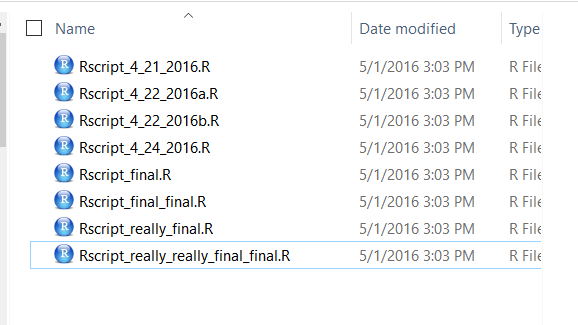
\includegraphics{img/MessySaves.png}
  When you open your repository, you only see the most recent version. But, it easy to compare versions, and you can easily revert to previous versions.
\item
  Improves collaborative efforts. Different researchers can work on the same files at the same time!
\item
  It is easy to share and distribute files through the Github website.
\item
  Your files are available anywhere, you just need internet connection!
\end{enumerate}

\hypertarget{what-are-git-and-github}{%
\subsection{What are Git and Github?}\label{what-are-git-and-github}}

\begin{itemize}
\item
  \textbf{Git} is a version control system that lets you track changes to files over time. These files can be any kind of file (eg .doc, .pdf, .xls), but free text differences are most easily visible (eg txt, csv, md).
\item
  \textbf{Github} is a website for storing your git versioned files remotely. It has many nice features to be able visualize differences between \href{https://help.github.com/articles/rendering-and-diffing-images/}{images}, \href{https://help.github.com/articles/mapping-geojson-files-on-github/}{rendering} \& \href{https://github.com/blog/1772-diffable-more-customizable-maps}{diffing} map data files, \href{https://help.github.com/articles/rendering-csv-and-tsv-data/}{render text data files}, and \href{https://help.github.com/articles/rendering-differences-in-prose-documents/}{track changes in text}.
\end{itemize}

Github was developed for social coding (i.e., sort of like an open source Wikipedia for programmers). Consequently, much of the functionality and terminology of Github (e.g., branches and pull requests) isn't necessary for a new R user getting started.

These concepts are more important for coders who want the entire coding community (and not just people working on the same project) to be able to suggest changes to their code. This isn't how most new R users will use Github.

To get the full functionality of Github, you will eventually want to learn other concepts. But, this can wait.

\hypertarget{some-github-terminology}{%
\subsection{Some Github terminology}\label{some-github-terminology}}

\begin{itemize}
\tightlist
\item
  \textbf{User}: A Github account for you (e.g., jules32).
\item
  \textbf{Organization}: The Github account for one or more user (e.g., datacarpentry).
\item
  \textbf{Repository}: A folder within the organization that includes files dedicated to a project.
\item
  \textbf{Local Github}: Copies of Github files located your computer.
\item
  \textbf{Remote Github}: Github files located on the \url{https://github.com} website.
\item
  \textbf{Clone}: Process of making a local copy of a remote Github repository. This only needs to be done once (unless you mess up your local copy).
\item
  \textbf{Pull}: Copy changes on the remote Github repository to your local Github repository. This is useful if multiple people are making changes to a repository.
\item
  \textbf{Push}: Save local changes to remote Github
\end{itemize}

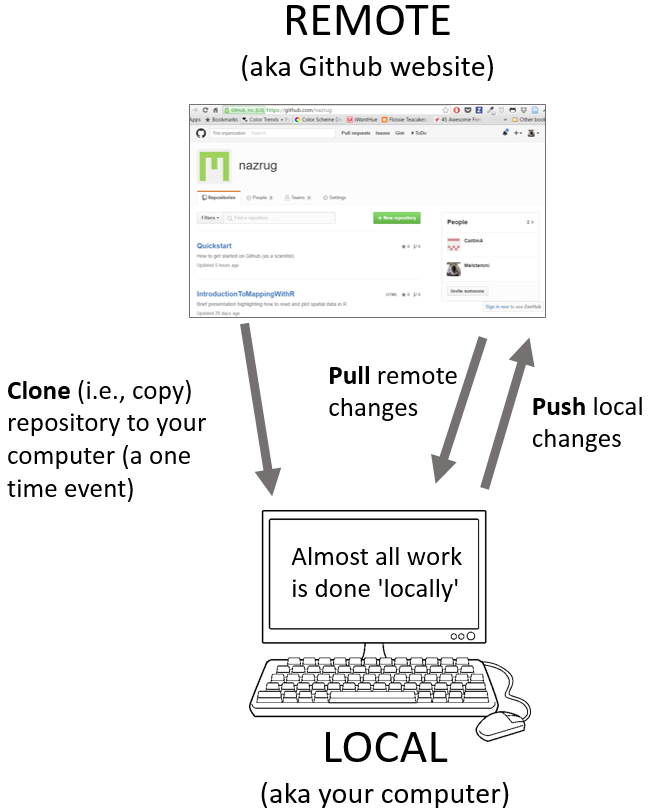
\includegraphics{img/push_pull_clone.png}

\hypertarget{create-a-repository-on-github.com}{%
\section{Create a repository on Github.com}\label{create-a-repository-on-github.com}}

First, go to your account on github.com and click ``New repository''.
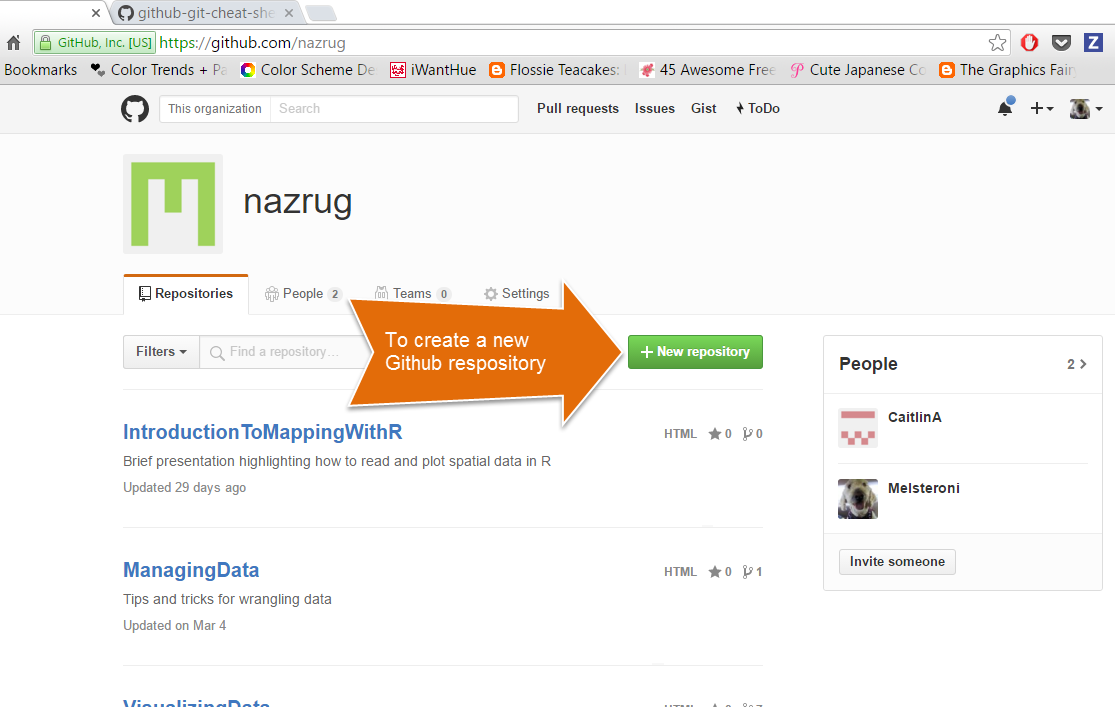
\includegraphics{img/create_repository.png}

Choose a name. Call it whatever you want (the shorter the better), or follow me for convenience. I will call mine \texttt{r-workshop}.

Also, add a description, make it public, create a README file, and create your repo!
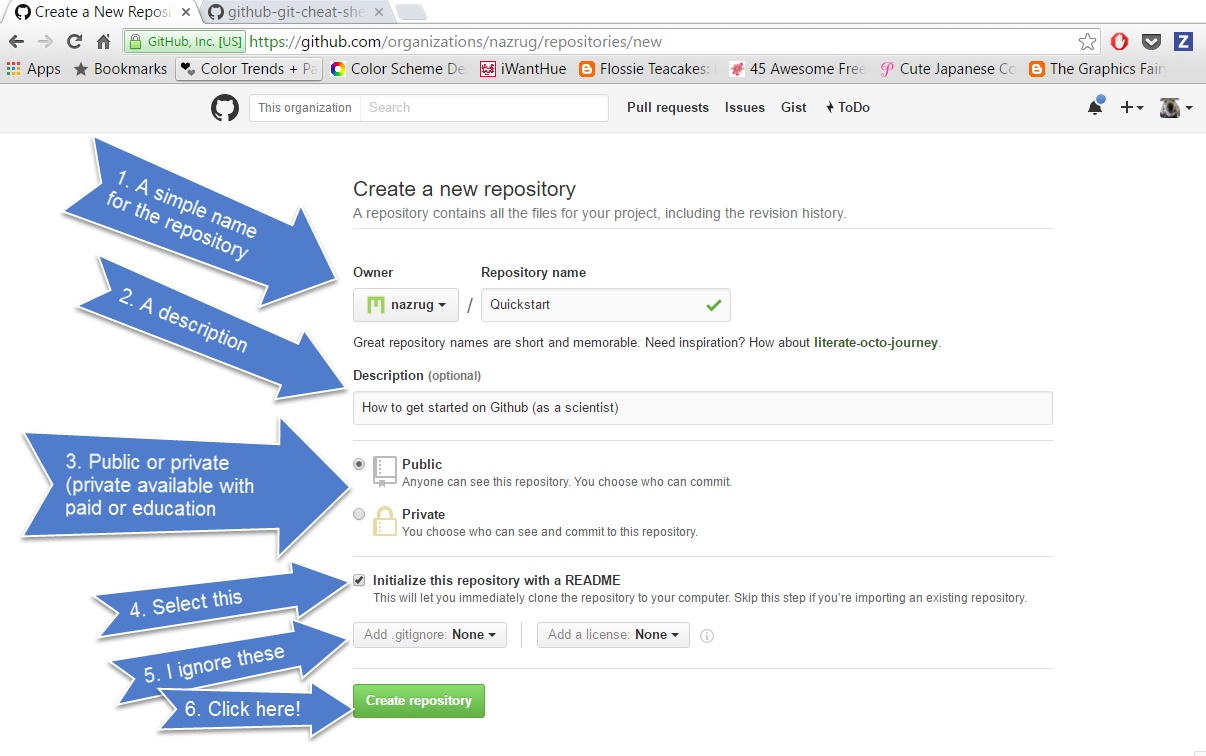
\includegraphics{img/create_repository_2.png}

The \emph{Add gitignore} option adds a document where you can identify files or file-types you want Github to ignore. These files will stay in on the local Github folder (the one on your computer), but will not be uploaded onto the web version of Github.

The \emph{Add a license} option adds a license that describes how other people can use your Github files (e.g., open source, but no one can profit from them, etc.). We won't worry about this today.

Check out our new repository!

Notice how the README.md file we created is automatically displayed at the bottom. The .md means that it is Markdown (remember how .Rmd was RMarkdown?) so the formatting we learned in the last lesson apply here.

\includegraphics{img/new_repository.png}

\hypertarget{create-a-gh-pages-branch}{%
\section{Create a gh-pages branch}\label{create-a-gh-pages-branch}}

We aren't going to talk about branches very much, but they are a powerful feature of git/GitHub. I think of it as creating a copy of your work that becomes a parallel universe that you can modify safely because it's not affecting your original work. And then you can choose to merge the universes back together if and when you want. By default, when you create a new repo you begin with one branch, and it is named \texttt{master}. When you create new branches, you can name them whatever you want. However, if you name one \texttt{gh-pages} (all lowercase, with a \texttt{-} and no spaces), this will let you create a website. And that's our plan. So, let's do this to create a \texttt{gh-pages} branch:

On the homepage for your repo on GitHub.com, click the button that says ``Branch:master''. Here, you can switch to another branch (right now there aren't any others besides \texttt{master}), or create one by typing a new name.

Let's type \texttt{gh-pages}.

Let's also change \texttt{gh-pages} to the default branch and delete the master branch: this will be a one-time-only thing that we do here:

First click to control branches:

And then click to change the default branch to \texttt{gh-pages}. I like to then delete the \texttt{master} branch when it has the little red trash can next to it. It will make you confirm that you really want to delete it, which I do!

\textbf{From here, you will work locally (on your computer).}

\hypertarget{clone-your-repository-using-rstudio}{%
\section{Clone your repository using RStudio}\label{clone-your-repository-using-rstudio}}

We'll start of by cloning to our local computer using RStudio. We are going to be cloning a copy of our Remote repository on Github.com to our local computers. Unlike downloading, cloning keeps all the version control and user information bundled with the files.

\textbf{Step 0}: Create your \texttt{github} folder

This is really important! We need to be organized and deliberate about where we want to keep all of our GitHub repositories (since this is the first of many in your career).

Let's all make a folder called \texttt{github} (all lowercase!) in our home directories. So it will look like this:

\begin{itemize}
\tightlist
\item
  Windows: \texttt{Users\textbackslash{}{[}User{]}\textbackslash{}Documents\textbackslash{}github\textbackslash{}}
\item
  Mac: \texttt{Users/{[}User{]}/github/}
\end{itemize}

This will let us take advantage of something that is really key about GitHub.com: you can easily navigate through folders within repositories and the urls reflect this navigation. The greatness of this will be evident soon. So let's set ourselves up for easily translating (and remembering) those navigation paths by having a folder called \texttt{github} that will serve as our `github.com'.

So really. Make sure that you have an all-lowercase folder called \texttt{github} in your home directory!!

\textbf{Step 1}: Copy the web address of the repository you want to clone.

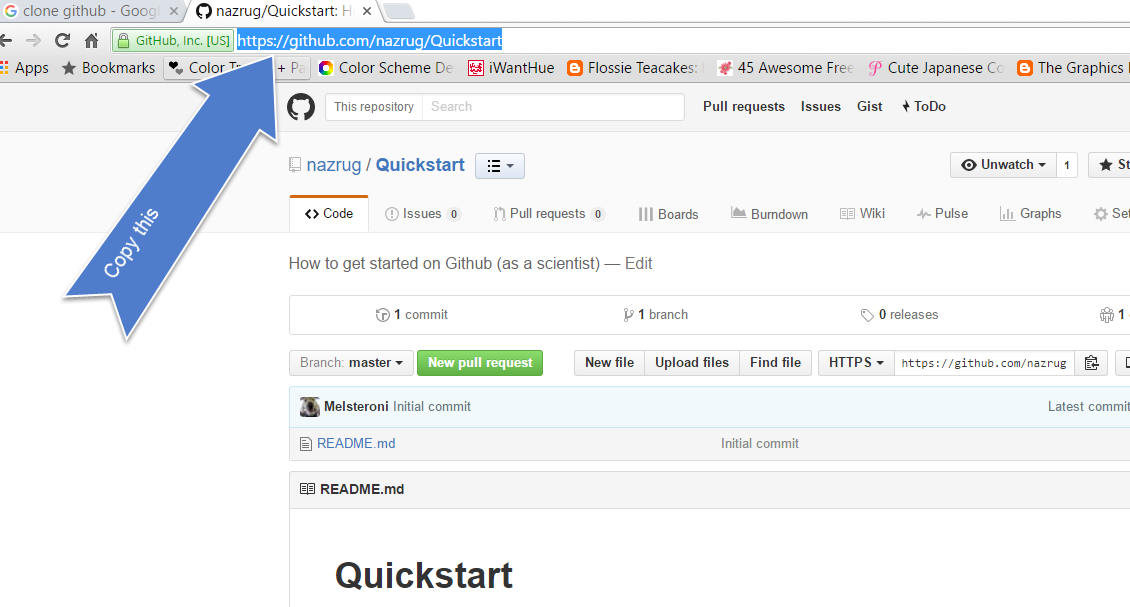
\includegraphics{img/clone_step1.png}

\textbf{Step 2}: from RStudio, go to New Project (also in the File menu).

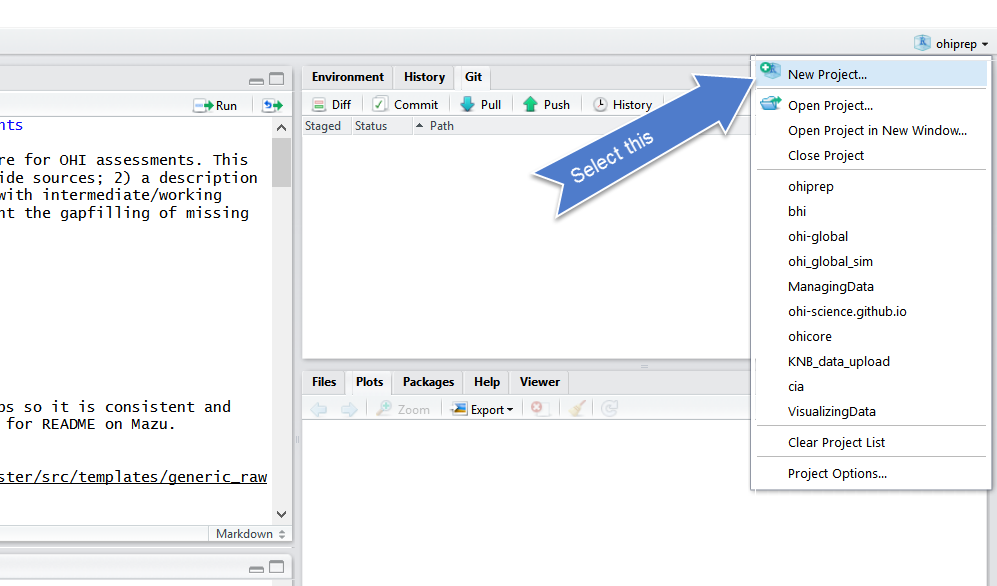
\includegraphics{img/new_project_1.png}

\textbf{Step 3}: Select Version Control

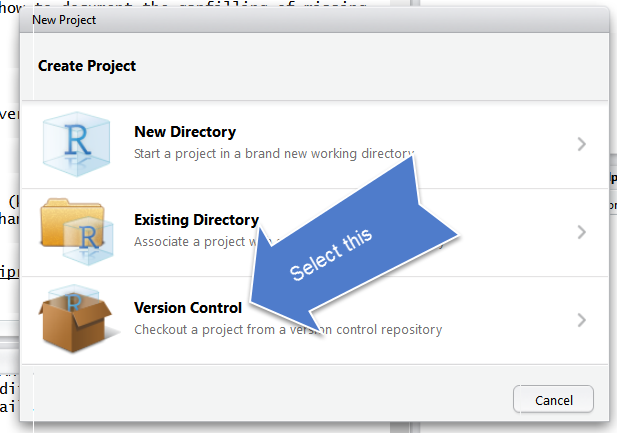
\includegraphics{img/new_project_2.png}

\textbf{Step 4}: Select Git

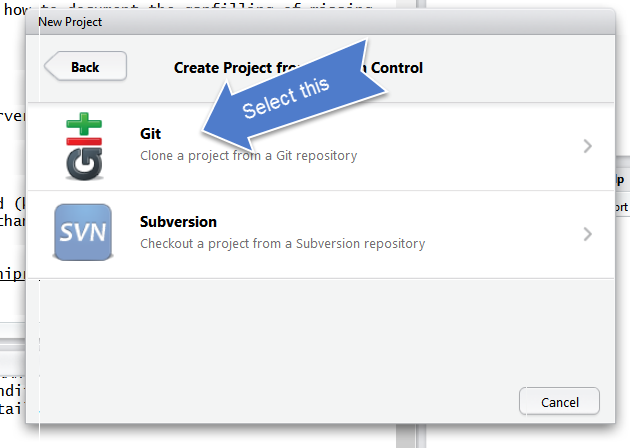
\includegraphics{img/new_project_3.png}

\textbf{Step 5}: Paste it in the Repository URL field, and type \textbf{tab} to autofill the Project Directory name. Make sure you keep the Project Directory Name \textbf{THE SAME} as the repository name from the URL.

Save it in your github folder (click on Browse) to do this.

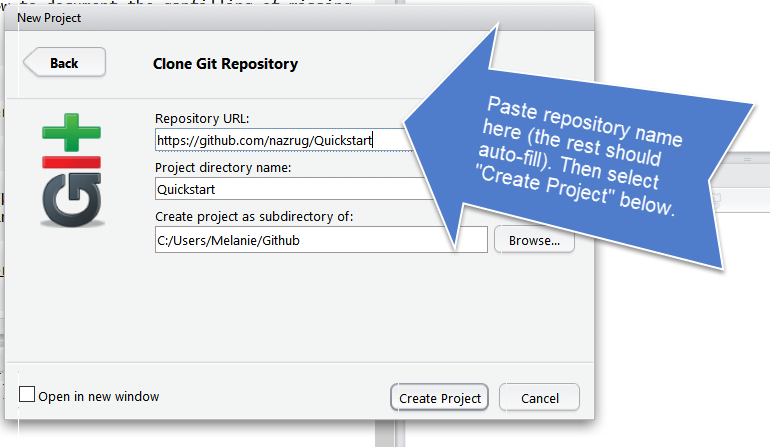
\includegraphics{img/new_project_4.png}

If everything went well, the repository will be added to the list located here:
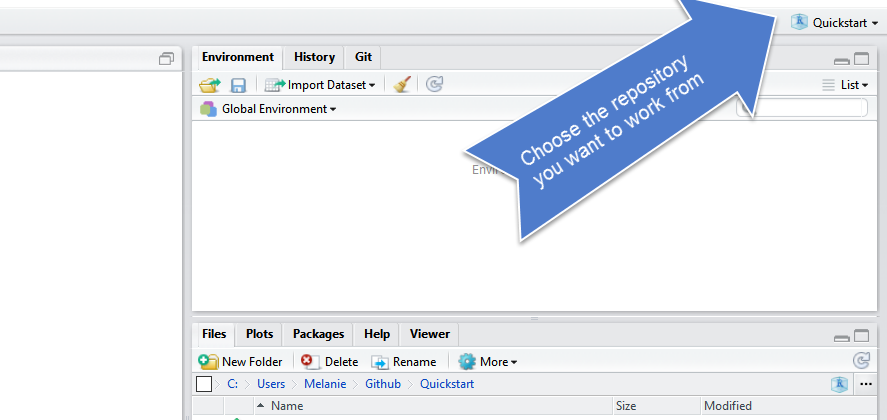
\includegraphics{img/select_project.png}

And the repository will be saved to the Github folder on your computer:

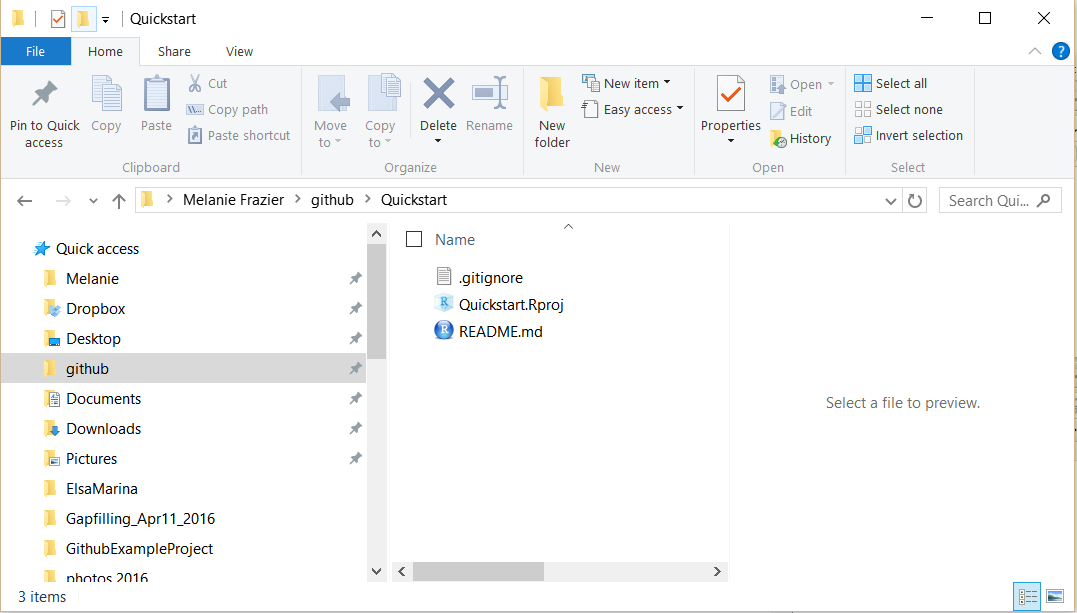
\includegraphics{img/cloned_repository.png}

Ta da!!!! The folder doesn't contain much of interest, but we are going to change that.

\hypertarget{inspect-your-repository}{%
\section{Inspect your repository}\label{inspect-your-repository}}

Notice a few things in our repo here:

\begin{enumerate}
\def\labelenumi{\arabic{enumi}.}
\tightlist
\item
  Our working directory is set to \texttt{\textasciitilde{}/github/r-workshop}. This means that I can start working with the files I have in here without setting the filepath. This is that when we cloned this from RStudio, it created an RStudio project, which you can tell because:

  \begin{itemize}
  \tightlist
  \item
    \texttt{.RProj} file, which you can see in the Files pane.
  \item
    The project is named in the top right hand corner
  \end{itemize}
\item
  We have a git tab! This is how we will interface directly to Github.com
\end{enumerate}

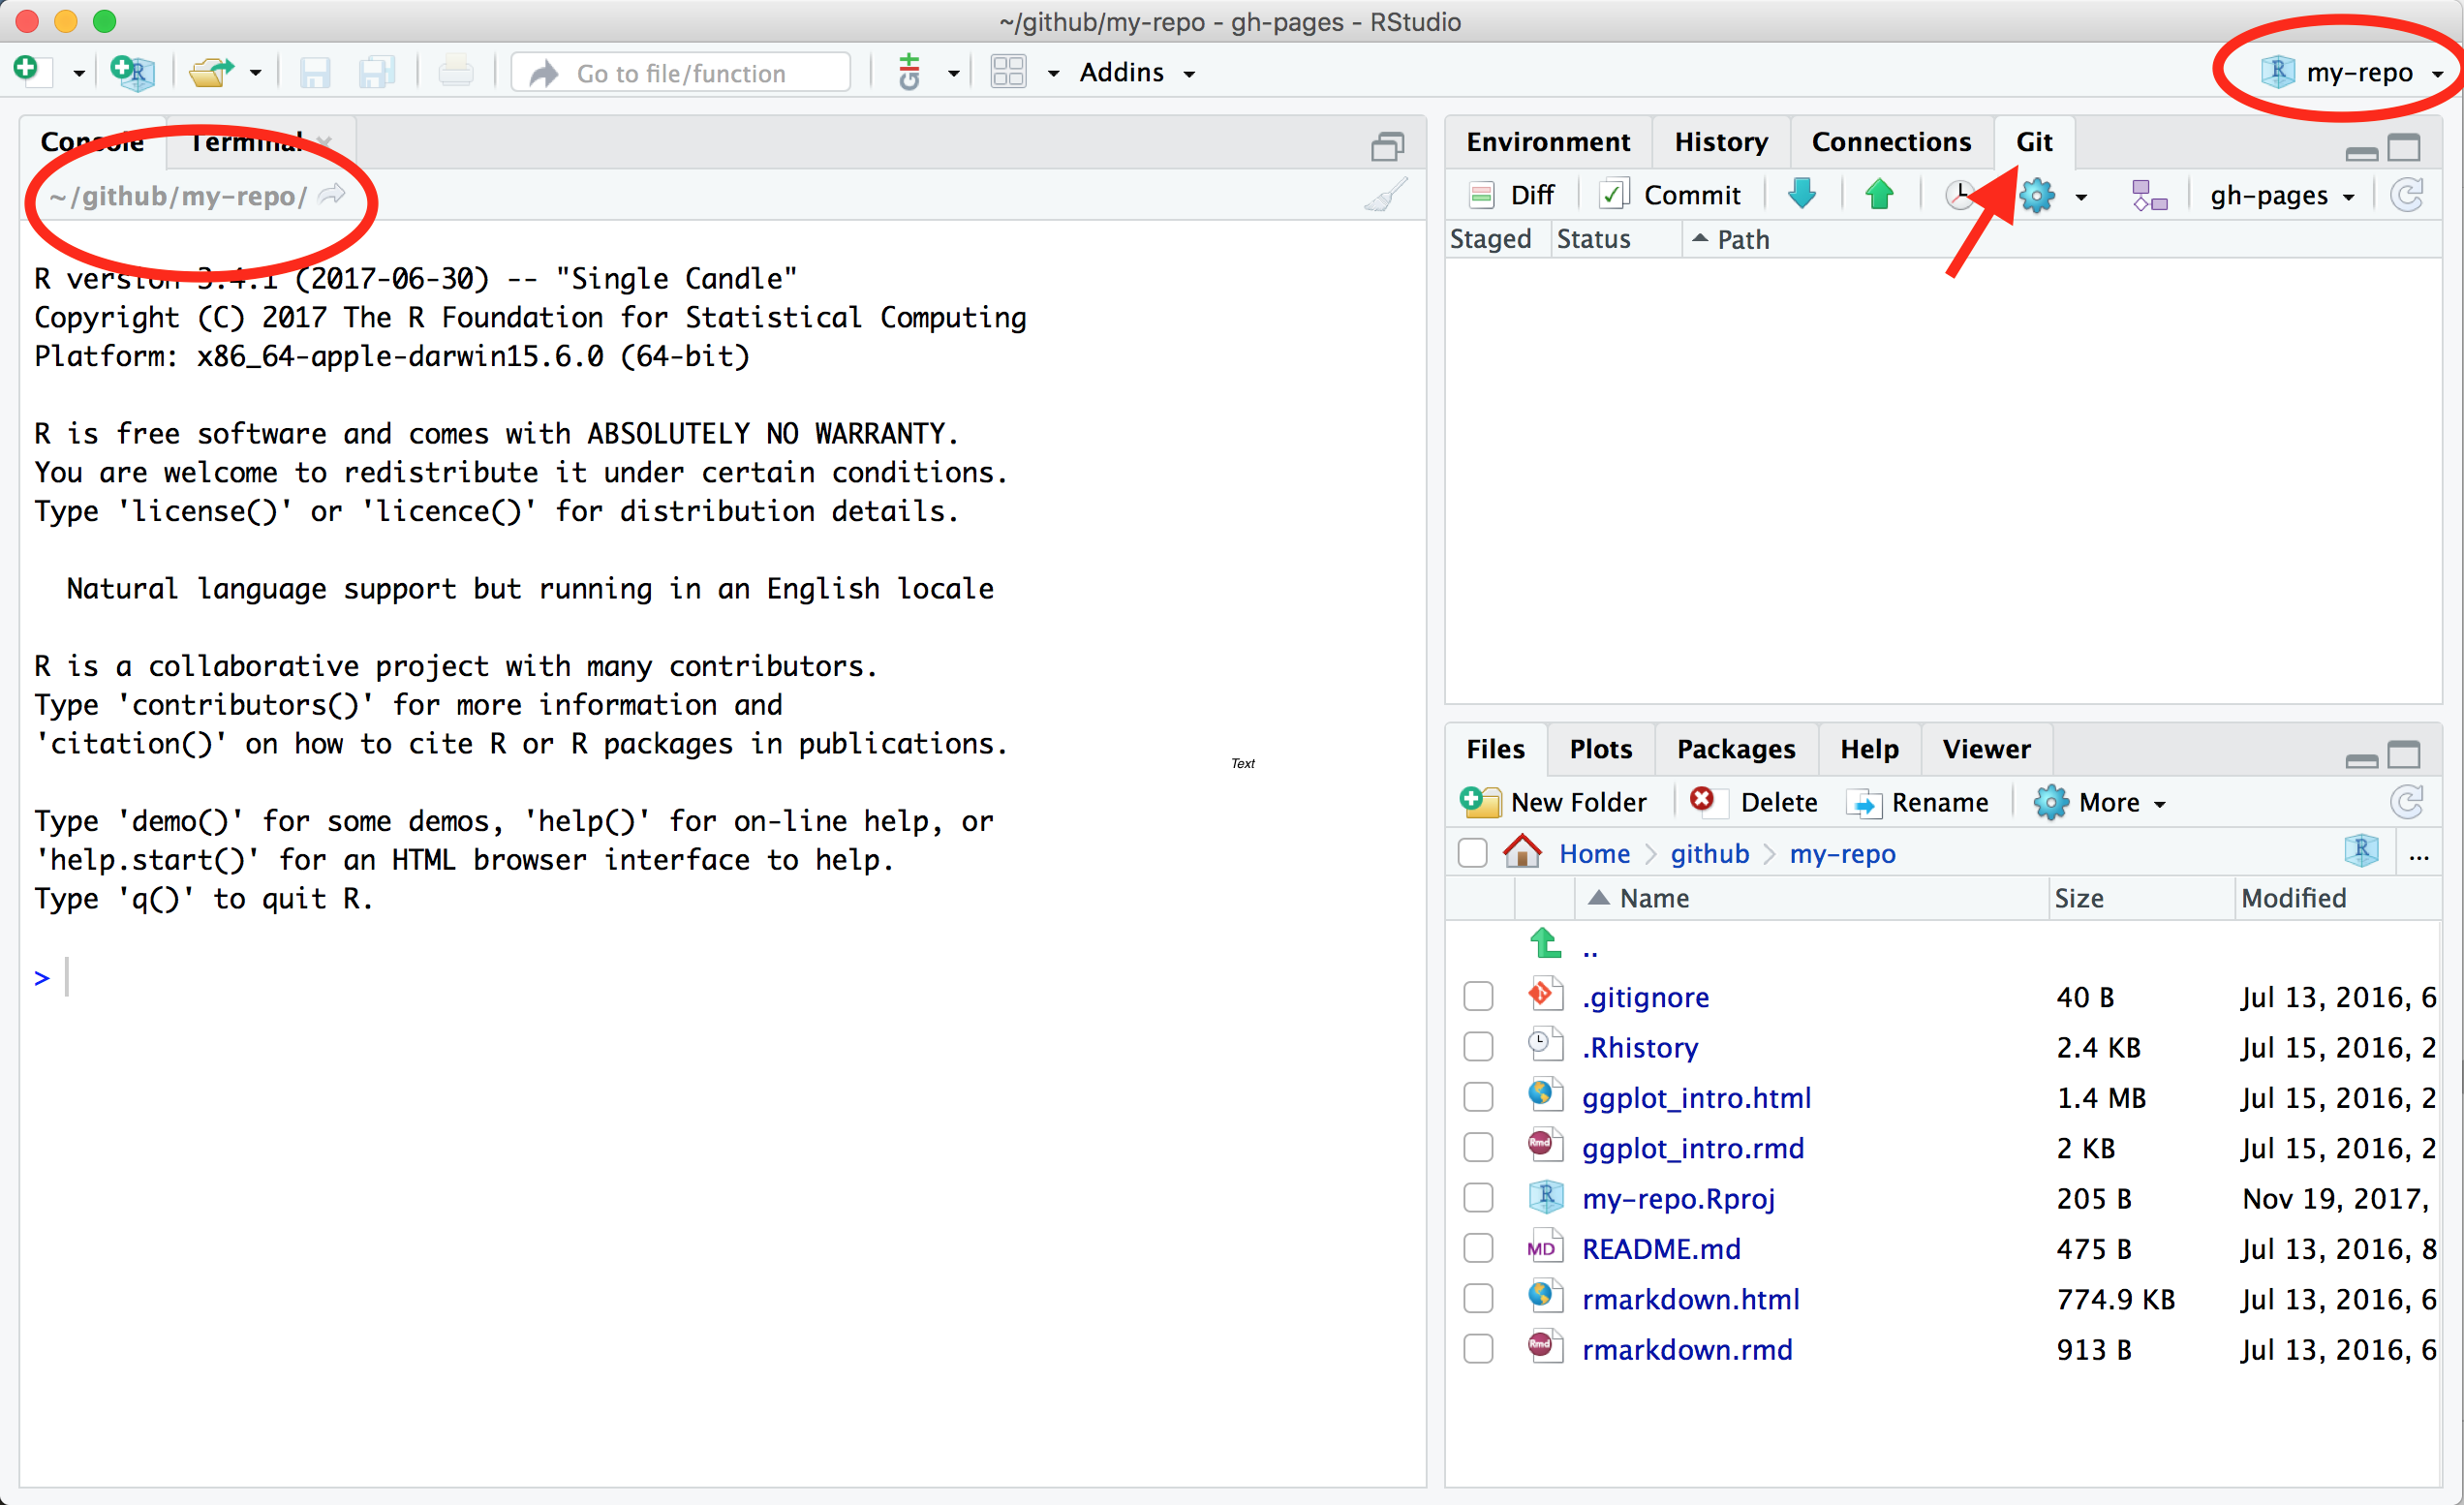
\includegraphics{img/RStudio_IDE_git.png}

When you first clone a repo through RStudio, RStudio will add an \texttt{.Rproj} file to your repo. And if you didn't add a \texttt{.gitignore} file when you originally created the repo on GitHub.com, RStudio will also add this for you. These will show up with little yellow \texttt{?} icons in your git tab. This is GitHub's way of saying: ``I am responsible for tracking everything that happens in this repo, but I haven't seen these files yet. Do you want me to track them too?'' (We'll see that when you click the box to stage them, they will turn into \texttt{A}s because they have been added to the repo.

\hypertarget{add-files-to-our-local-repo}{%
\section{Add files to our local repo}\label{add-files-to-our-local-repo}}

The repository will contain:

\begin{itemize}
\tightlist
\item
  .gitignore file
\item
  README.md
\item
  Rproj
\end{itemize}

Let's create the following:

\begin{itemize}
\tightlist
\item
  folder called ``data''
\item
  folder called ``figures''
\end{itemize}

They both show up in your Finder! \ldots{}

\hypertarget{get-data-files-into-your-working-directory}{%
\subsection{Get data files into your working directory}\label{get-data-files-into-your-working-directory}}

In Session 1, we introduced how and why R Projects are great for reproducibility, because our self-contained working directory will be the \textbf{first} place R looks for files.

You downloaded several files for this workshop, some comma separate value (CSV) files and some as Excel spreadsheets (.xlsx):

\begin{itemize}
\tightlist
\item
  fish\_counts\_curated.csv
\item
  invert\_counts\_curated.xlsx
\item
  kelp\_counts\_curated.xlsx
\item
  substrate\_cover\_curated.xlsx
\item
  lobsters.xlsx
\item
  lobsters2.xlsx
\item
  ca\_np.csv
\item
  ci\_np.xlsx
\end{itemize}

Copy and paste those files into the `data' subfolder of your R project. Notice that now these files are in your working directory when you go back to that Project in RStudio (check the `Files' tab and navigate to the data subfolder). That means they're going to be in the first place R will look when you ask it to find a file to read in.

I'm going to go to the Finder (Windows Explorer on a PC) and copy a file into my repository from there. And then I'm going to go back to RStudio -- it shows up in the git tab! So the repository is being tracked, no matter how you make changes to it (changes do not have to be done only through RStudio).

To make changes to the repository, you will work from your computer (``local Github'').

When files are changed in the local repository, these changes will be reflected in the Git tab of RStudio:

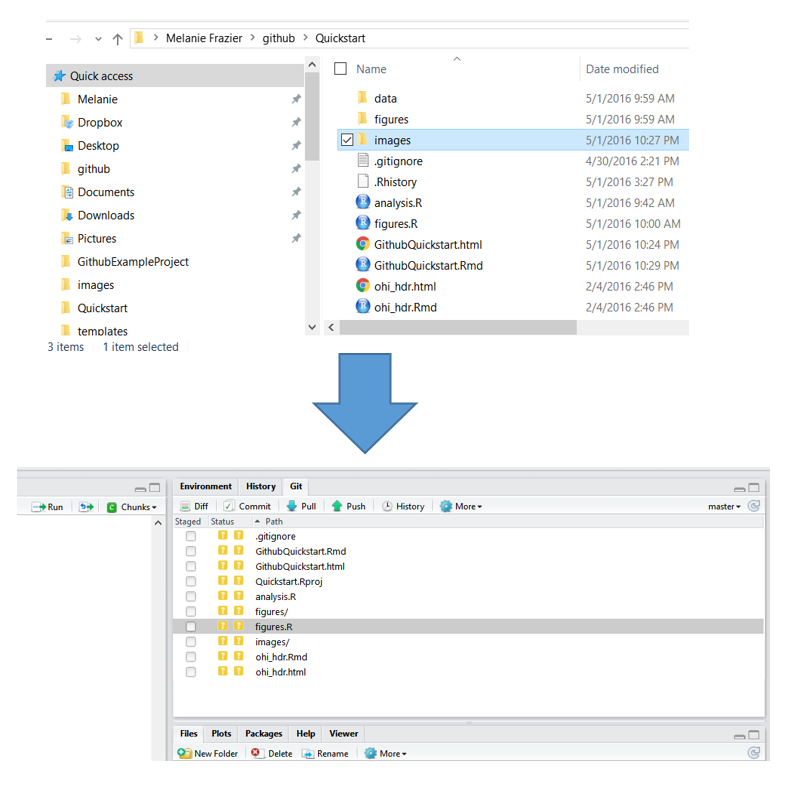
\includegraphics{img/modify_files.png}

\hypertarget{inspect-what-has-changed}{%
\subsection{Inspect what has changed}\label{inspect-what-has-changed}}

These are the codes RStudio uses to describe how the files are changed, (from the RStudio \href{http://www.rstudio.com/wp-content/uploads/2016/01/rstudio-IDE-cheatsheet.pdf}{cheatsheet}):
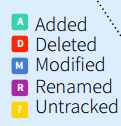
\includegraphics{img/modified.png}

\hypertarget{sync-from-rstudio-to-github}{%
\section{Sync from RStudio to GitHub}\label{sync-from-rstudio-to-github}}

When you are ready to commit your changes, you follow these steps:

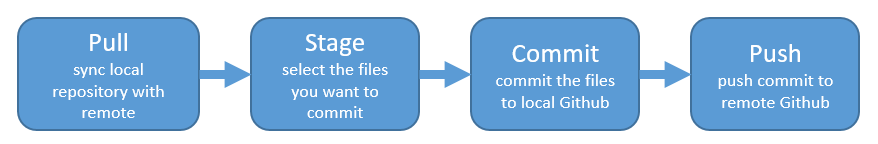
\includegraphics{img/commit_overview.png}

We walk through this process below:

\hypertarget{pull}{%
\subsection{Pull}\label{pull}}

From the Git tab, ``Pull'' the repository. This makes sure your local repository is synced with the remote repository. This is very important if other people are making changes to the repository or if you are working from multiple computers.

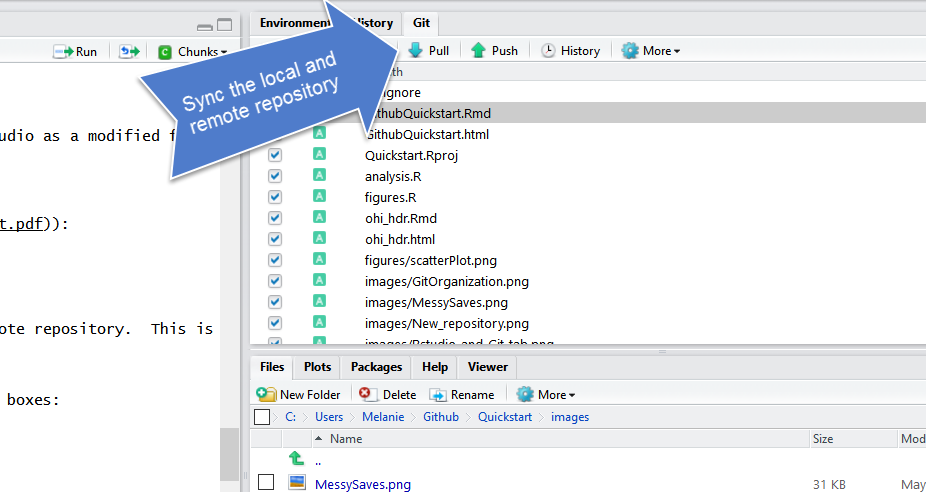
\includegraphics{img/pull.png}

\hypertarget{stage}{%
\subsection{Stage}\label{stage}}

Stage the files you want to commit. In RStudio, this involves checking the ``Staged'' boxes:

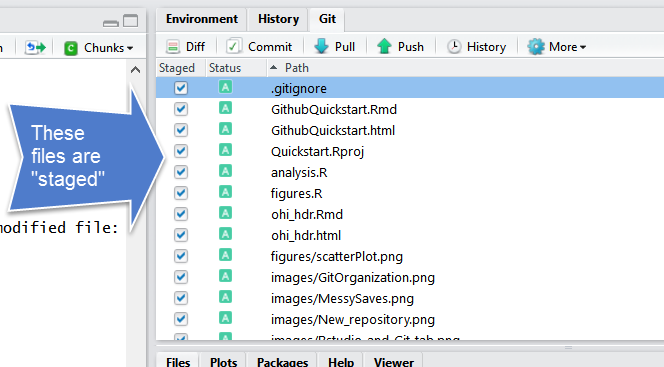
\includegraphics{img/staged.png}

\hypertarget{commit}{%
\subsection{Commit}\label{commit}}

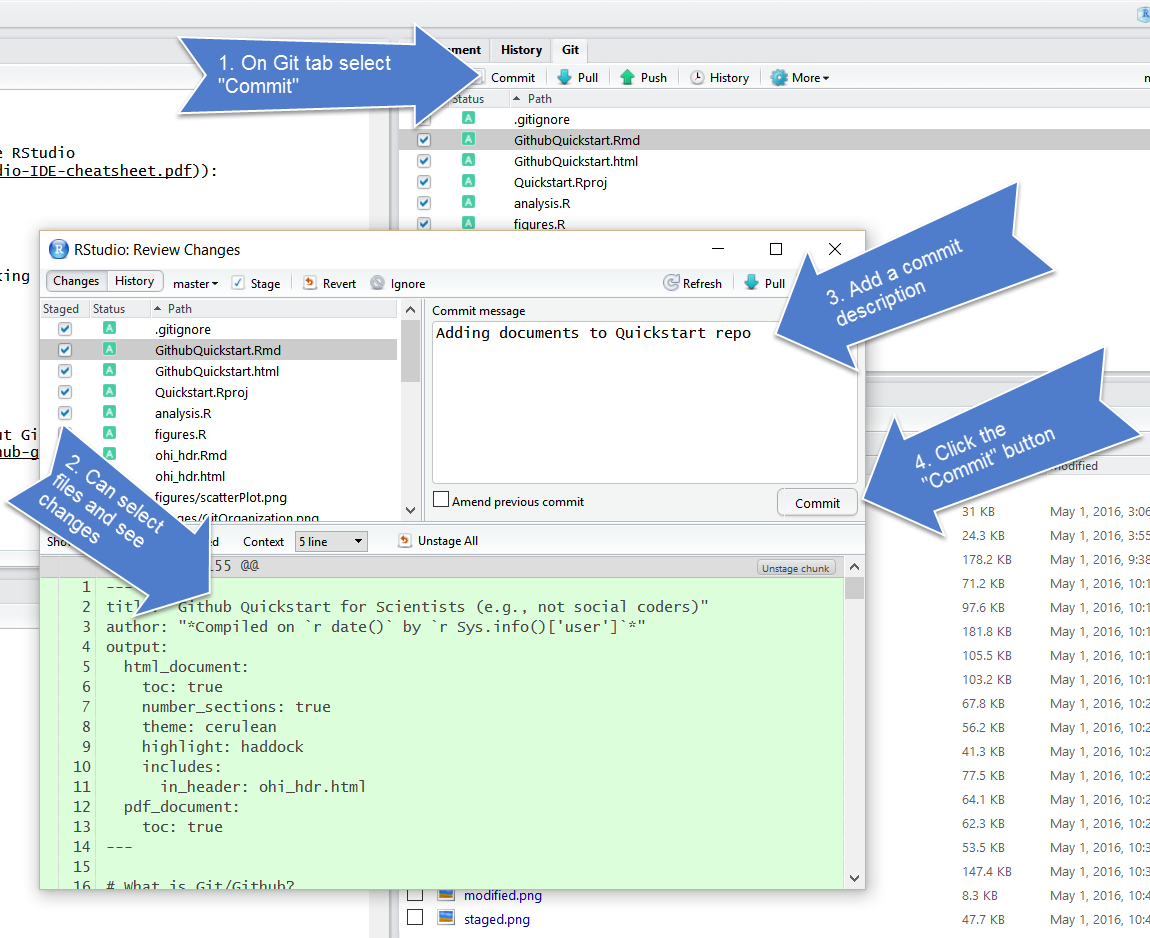
\includegraphics{img/commit.png}

\hypertarget{push}{%
\subsection{Push}\label{push}}

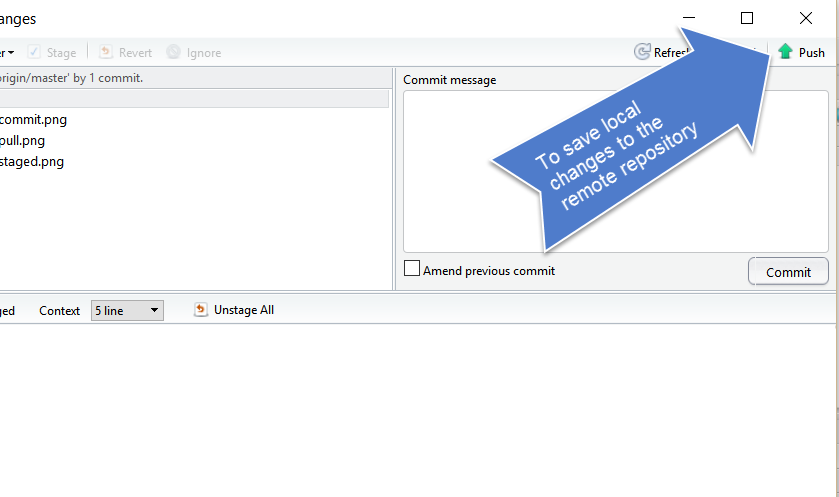
\includegraphics{img/push.png}

\hypertarget{explore-remote-github}{%
\section{Explore remote Github}\label{explore-remote-github}}

The files you added should be on github.com:

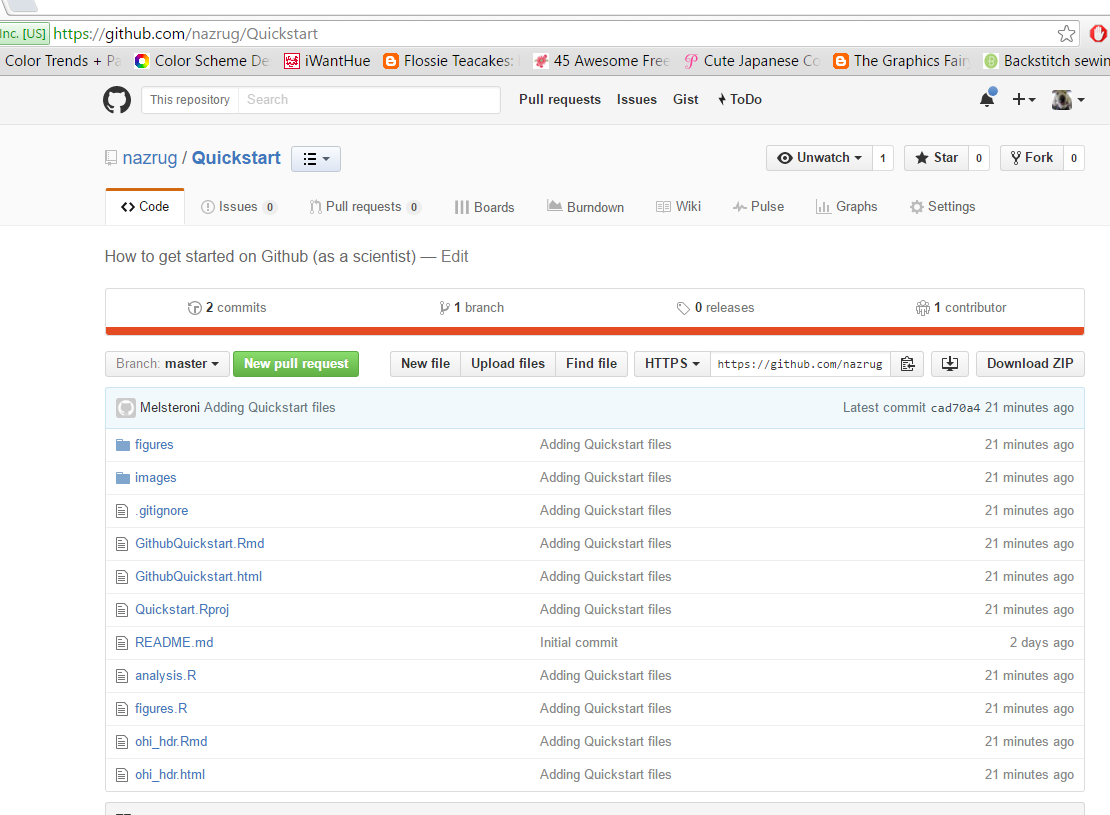
\includegraphics{img/Github_remote.png}

Let's also explore commit history, file history.

\hypertarget{activity-1}{%
\subsection{Activity}\label{activity-1}}

Go back to RStudio.

This time let's edit an existing file instead of adding something new. Open your README file by clicking on it in the Files pane (lower right corner). Write a few lines of text (like your dog's name), save, and see what happens in your Git Tab. Sync it to your remote repository at Github.com.

\hypertarget{create-a-new-r-markdown-file}{%
\section{Create a new R Markdown file}\label{create-a-new-r-markdown-file}}

Now get ourselves back into learning R. We are going to use R Markdown so that you can write notes to yourself in Markdown, and have a record of all your R code. Writing R commands in the console like we did this morning is great, but limited; it's hard to keep track of and hard to efficiently share with others. Plus, as your analyses get more complicated, you need to be able to see them all in one place.

Go to File \textgreater{} New File \textgreater{} R Markdown \ldots{} (or click the green plus in the top left corner).

Let's set up this file so we can use it for the rest of the day. I'm going to delete all the text that is already there and write some new text.

This will be your notes for the next session.

Here's what I'm going to write in my R Markdown file to begin:

\begin{verbatim}
---
title: "Reading data into R with `readxl`"
author: "Julie Lowndes"
date: "12/7/2019"
output: html_document
---

# Learning `readxl`

We are working with data and it's going to be amazing.
\end{verbatim}

Now, let's save it. I'm going to call my file \texttt{readxl.Rmd}. You can knit it if you'd like.

Then, knit your file, and sync your file to GitHub: commit and pull

What if a file doesn't show up in the Git tab and you expect that it should? Check to make sure you've saved the file. If the filename is red with an asterix, there have been changes since it was saved. Remember to save before syncing to GitHub!

\hypertarget{explore-your-webpage}{%
\section{Explore your webpage}\label{explore-your-webpage}}

You've just created a webpage!

It will exist at this url: username.github.io/repo-name/filename. Mine is: jules32.github.io/r-workshop/readxl.

\begin{quote}
\textbf{\emph{ProTip}} Pay attention to URLs. An unsung skill of the modern analyst is to be able to navigate the internet by keeping an eye on patterns.
\end{quote}

Troubleshooting:

\begin{itemize}
\tightlist
\item
  404 error? Remove trailing / from the url
\item
  Wants you to download? Remove trailing .Rmd from the url
\end{itemize}

\hypertarget{committing---how-often-tracking-changes-in-your-files}{%
\section{Committing - how often? Tracking changes in your files}\label{committing---how-often-tracking-changes-in-your-files}}

Whenever you make changes to the files in Github, you will walk through the Pull -\textgreater{} Stage -\textgreater{} Commit -\textgreater{} Push steps.

I tend to do this every time I finish a task (basically when I start getting nervous that I will lose my work). Once something is committed, it is very difficult to lose it.

One thing that I love about about Github is that it is easy to see how files have changed over time. Usually I compare commits through github.com:

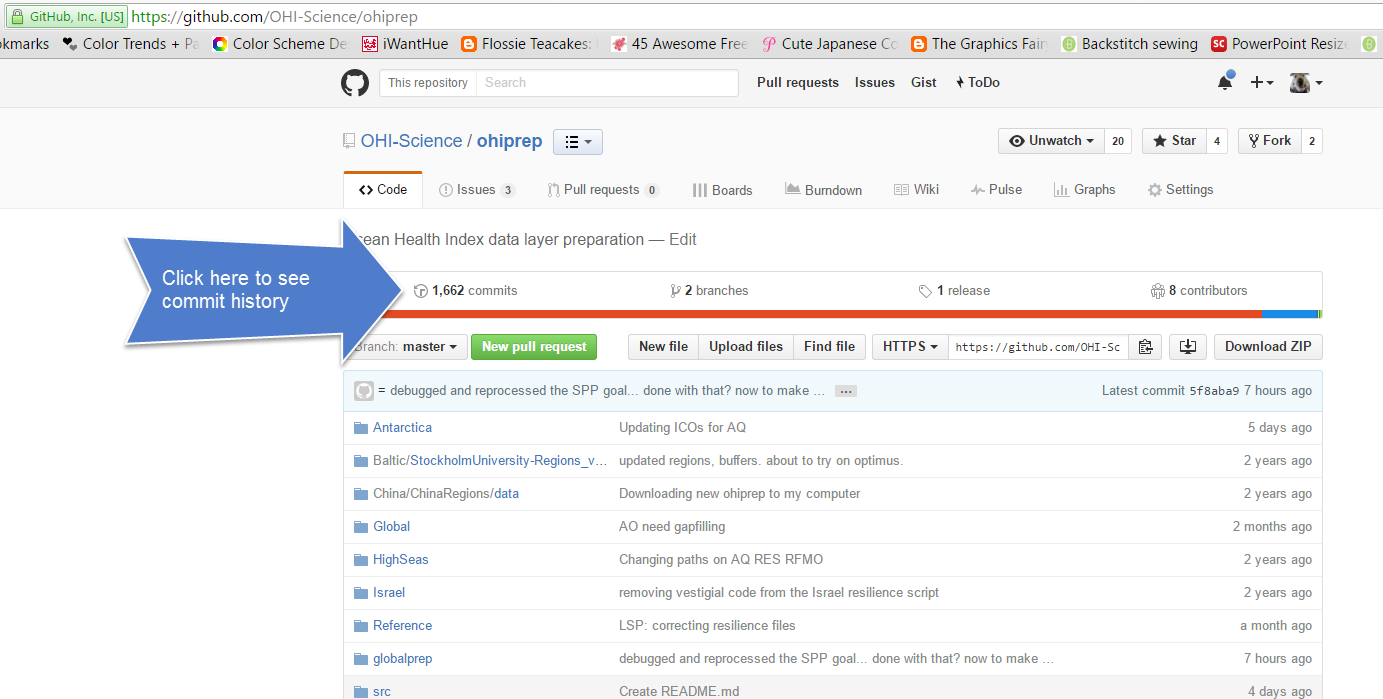
\includegraphics{img/commit_history.png}

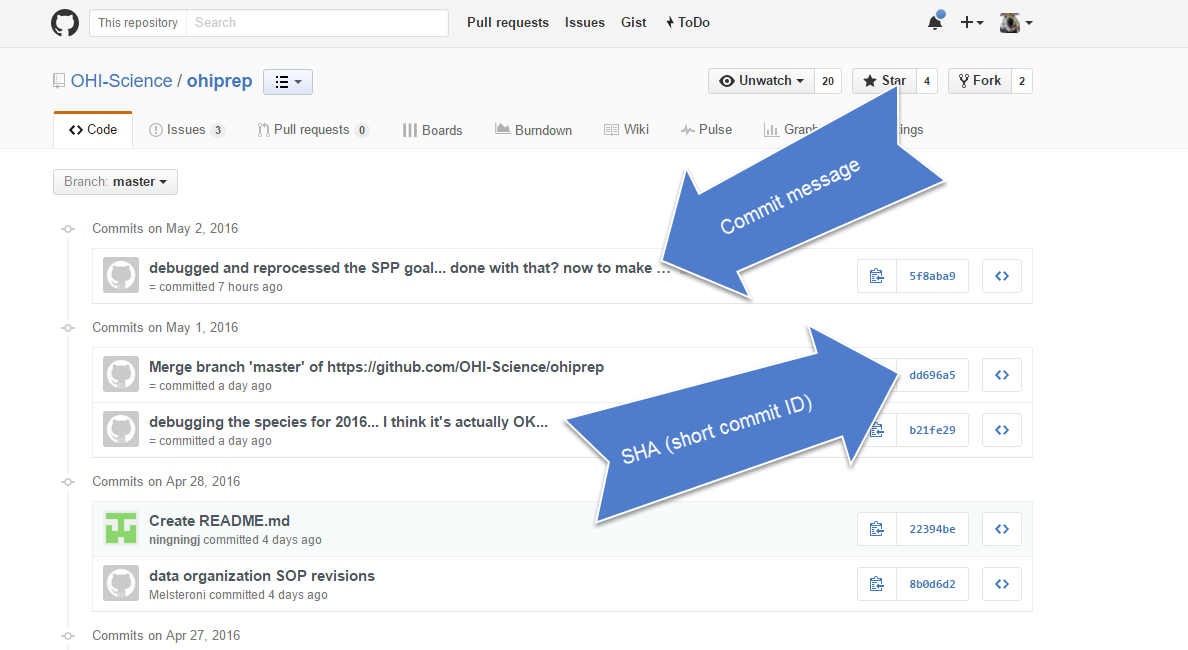
\includegraphics{img/commit_compare_2.png}

You can click on the commits to see how the files changed from the previous commit:

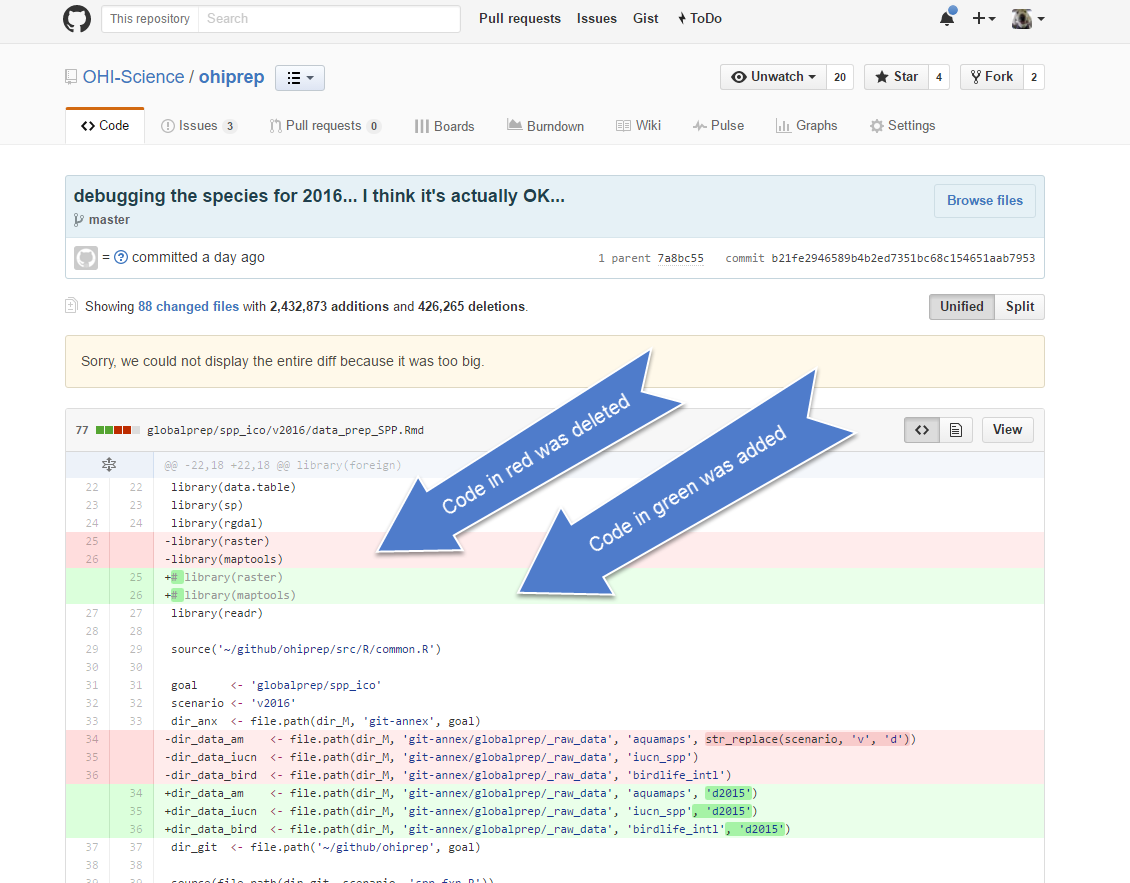
\includegraphics{img/commit_compare_3.png}

\hypertarget{happy-git-with-r}{%
\section{Happy Git with R}\label{happy-git-with-r}}

If you have problems, we'll help you out using Jenny Bryan's \href{http://happygitwithr.com}{HappyGitWithR}, particularly the sections on \href{http://happygitwithr.com/rstudio-see-git.html}{Detect Git from RStudio} and \href{http://happygitwithr.com/troubleshooting.html}{RStudio, Git, GitHub Hell (troubleshooting)}. So as we are coming around, have a look at it and see if you can help troubleshoot too!

\hypertarget{efficiency-tips-1}{%
\section{Efficiency Tips}\label{efficiency-tips-1}}

\hypertarget{ggplot2}{%
\chapter{Graphs with ggplot2}\label{ggplot2}}

\hypertarget{summary-2}{%
\section{Summary}\label{summary-2}}

Now that we know how to \emph{get} some data, the next thing we'll probably want to do is look at it. In Excel, graphs are made by manually selecting options - which, as we've discussed previously, may not be the best option for reproducibility. Also, if we haven't built a graph with reproducible code, then we might not be able to easily recreate a graph \emph{or} use that code again to make the same style graph with different data.

Using \texttt{ggplot2}, the graphics package within the \texttt{tidyverse}, we'll write reproducible code to manually and thoughtfully build our graphs.

\begin{quote}
``ggplot2 implements the grammar of graphics, a coherent system for describing and building graphs. With ggplot2, you can do more faster by learning one system and applying it in many places.'' - \href{http://r4ds.had.co.nz/data-visualisation.html}{R4DS}
\end{quote}

So yeah\ldots{}that \texttt{gg} is from ``grammar of graphics.''

We'll use the \texttt{ggplot2} package, but the function we use to initialize a graph will be \texttt{ggplot}, which works best for data in tidy format (i.e., a column for every variable, and a row for every observation). Graphics with \texttt{ggplot} are built step-by-step, adding new elements as layers with a plus sign (\texttt{+}) between layers (note: this is different from the pipe operator, \texttt{\%\textgreater{}\%}. Adding layers in this fashion allows for extensive flexibility and customization of plots.

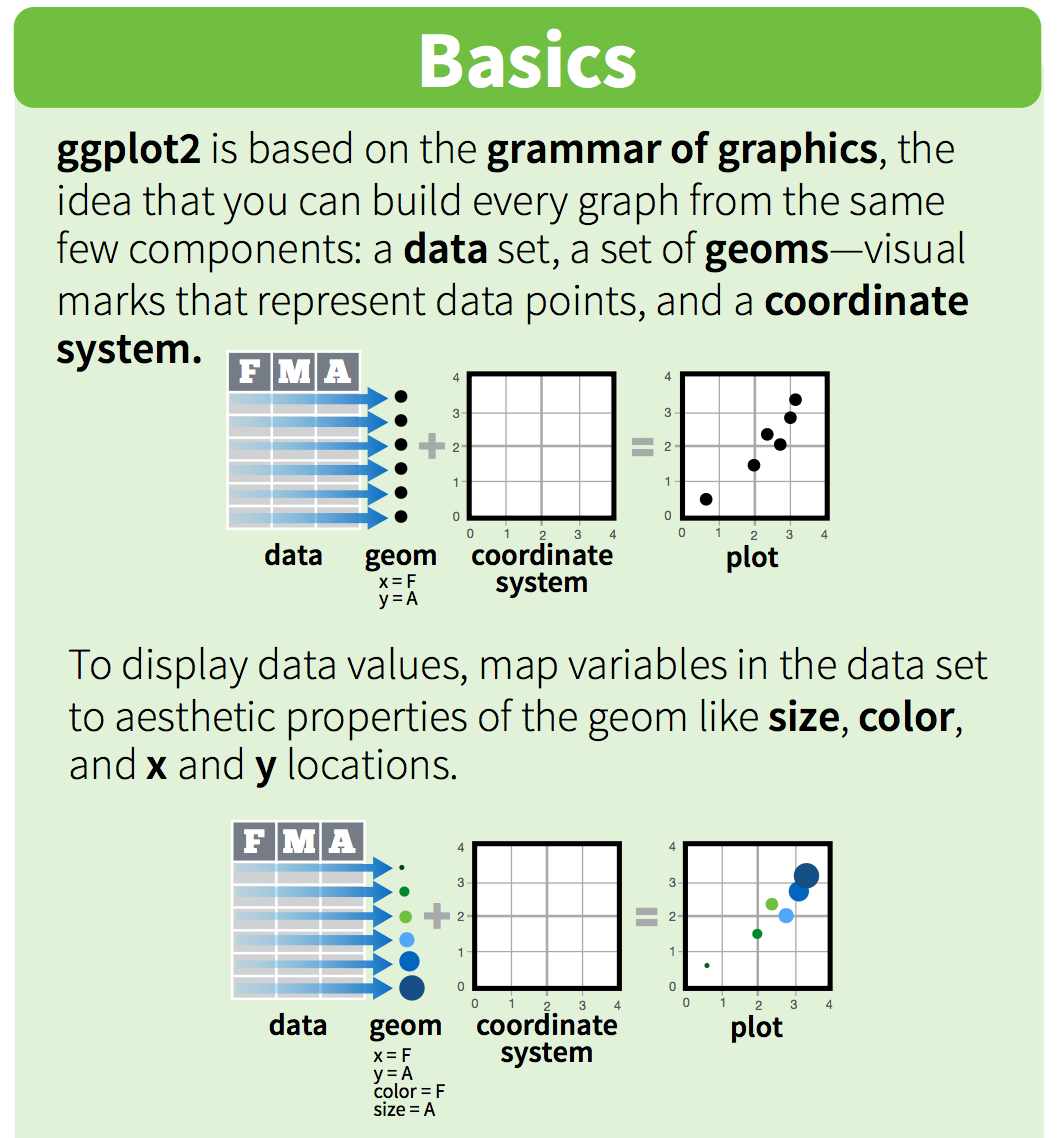
\includegraphics{img/rstudio-cheatsheet-ggplot.png}

\hypertarget{objectives-2}{%
\subsection{Objectives}\label{objectives-2}}

\begin{itemize}
\tightlist
\item
  Build several common types of graphs (scatterplot, column, line) in ggplot2
\item
  Customize gg-graph aesthetics (color, style, themes, etc.)
\item
  Update axis labels and titles
\item
  Combine compatible graph types (geoms)
\item
  Build multiseries graphs
\item
  Split up data into faceted graphs
\item
  Exporting figures with \texttt{ggsave()}
\end{itemize}

\hypertarget{resources-3}{%
\subsection{Resources}\label{resources-3}}

\begin{itemize}
\tightlist
\item
  \href{Chapter\%203\%20-\%20Data\%20Visualization\%20in\%20R\%20for\%20Data\%20Science\%20by\%20Grolemund\%20and\%20Wickham}{https://r4ds.had.co.nz/data-visualisation.html}
\item
  \href{https://www.rstudio.com/wp-content/uploads/2016/11/ggplot2-cheatsheet-2.1.pdf}{ggplot2-cheatsheet-2.1.pdf}\\
\item
  \href{http://www.cookbook-r.com/Graphs/\#graphs-with-ggplot2}{Graphs with ggplot2 - Cookbook for R}\\
\item
  \href{http://varianceexplained.org/r/why-I-use-ggplot2/}{``Why I use ggplot2'' - David Robinson Blog Post}
\end{itemize}

\hypertarget{getting-started---create-a-new-.rmd-attach-packages-get-data}{%
\section{Getting started - Create a new .Rmd, attach packages \& get data}\label{getting-started---create-a-new-.rmd-attach-packages-get-data}}

Within your existing version-controlled R project, create a new R Markdown document with title ``Data visualization with ggplot2.'' Remove everything below the first code chunk. Knit and save the .Rmd file within your project working directory as ``my\_ggplot2''.

The \texttt{ggplot2} package is part of the \texttt{tidyverse}, so we don't need to attach it separately. Attach the \texttt{tidyverse}, \texttt{readxl} and \texttt{here} packages in the top-most code chunk of your .Rmd.

\begin{Shaded}
\begin{Highlighting}[]
\KeywordTok{library}\NormalTok{(tidyverse)}
\KeywordTok{library}\NormalTok{(readxl)}
\KeywordTok{library}\NormalTok{(here)}
\end{Highlighting}
\end{Shaded}

In this session, we'll use data for parks visitation from two files:

\begin{itemize}
\tightlist
\item
  A comma-separated-value (CSV) file containing visitation data for all National Parks in California (ca\_np.csv)
\item
  A single Excel worksheet containing only visitation for Channel Islands National Park (ci\_np.xlsx)
\end{itemize}

Add a new code chunk to read in the data from the \textbf{data} subfolder within your working directory.

\begin{Shaded}
\begin{Highlighting}[]
\NormalTok{ca_np <-}\StringTok{ }\KeywordTok{read_csv}\NormalTok{(}\KeywordTok{here}\NormalTok{(}\StringTok{"data"}\NormalTok{, }\StringTok{"ca_np.csv"}\NormalTok{))}
\NormalTok{ci_np <-}\StringTok{ }\KeywordTok{read_xlsx}\NormalTok{(}\KeywordTok{here}\NormalTok{(}\StringTok{"data"}\NormalTok{, }\StringTok{"ci_np.xlsx"}\NormalTok{))}
\end{Highlighting}
\end{Shaded}

Let's take a quick look at the data to see what it contains. For example:

\begin{itemize}
\tightlist
\item
  \texttt{View()}: to look at the object in spreadsheet format
\item
  \texttt{names()}: to see the variable (column) names
\item
  \texttt{summary()}: see a quick summary of each variable
\end{itemize}

\hypertarget{our-first-ggplot-graph-visitors-to-channel-islands-np}{%
\section{Our first ggplot graph: Visitors to Channel Islands NP}\label{our-first-ggplot-graph-visitors-to-channel-islands-np}}

To create a bare-bones ggplot graph, we need to tell R three basic things:

\begin{enumerate}
\def\labelenumi{\arabic{enumi}.}
\tightlist
\item
  We're using \texttt{ggplot}
\item
  Data we're using \& variables we're plotting (i.e., what is x and/or y?)
\item
  What type of graph we're making (the type of \emph{geom})
\end{enumerate}

Generally, that structure will look like this:

\begin{Shaded}
\begin{Highlighting}[]
\KeywordTok{ggplot}\NormalTok{(}\DataTypeTok{data =}\NormalTok{ df_name, }\KeywordTok{aes}\NormalTok{(}\DataTypeTok{x =}\NormalTok{ x_var_name, }\DataTypeTok{y =}\NormalTok{ y_var_name)) }\OperatorTok{+}
\StringTok{  }\KeywordTok{geom_type}\NormalTok{()}
\end{Highlighting}
\end{Shaded}

Breaking that down:

\begin{itemize}
\tightlist
\item
  First, tell R you're using \texttt{ggplot()}
\item
  Then, tell it the object name where variables exist (\texttt{data\ =\ df\_name})
\item
  Next, tell it the aesthetics \texttt{aes()} to specify which variables you want to plot
\item
  Then add a layer for the type of geom (graph type) with \texttt{geom\_*()} - for example, \texttt{geom\_point()} is a scatterplot, \texttt{geom\_line()} is a line graph, \texttt{geom\_col()} is a column graph, etc.
\end{itemize}

Let's do that to create a line graph of visitors to Channel Islands National Park:

\begin{Shaded}
\begin{Highlighting}[]
\KeywordTok{ggplot}\NormalTok{(}\DataTypeTok{data =}\NormalTok{ ci_np, }\KeywordTok{aes}\NormalTok{(}\DataTypeTok{x =}\NormalTok{ year, }\DataTypeTok{y =}\NormalTok{ visitors)) }\OperatorTok{+}
\StringTok{  }\KeywordTok{geom_line}\NormalTok{()}
\end{Highlighting}
\end{Shaded}

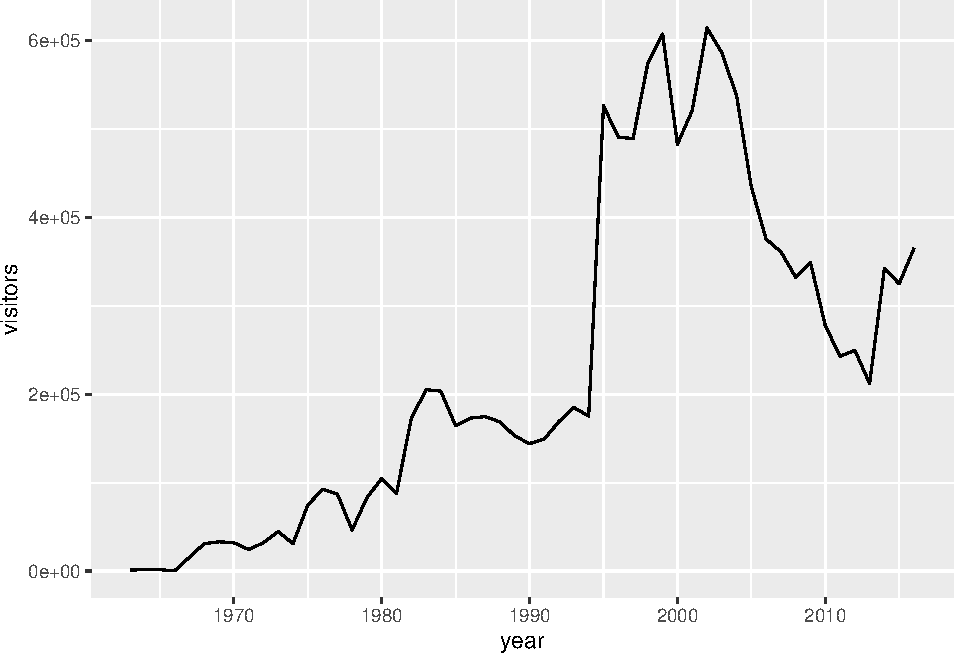
\includegraphics{R-for-Excel-Users_files/figure-latex/unnamed-chunk-30-1.pdf}

Or, we could change that to a scatterplot just by updating the \texttt{geom\_*}:

\begin{Shaded}
\begin{Highlighting}[]
\KeywordTok{ggplot}\NormalTok{(}\DataTypeTok{data =}\NormalTok{ ci_np, }\KeywordTok{aes}\NormalTok{(}\DataTypeTok{x =}\NormalTok{ year, }\DataTypeTok{y =}\NormalTok{ visitors)) }\OperatorTok{+}
\StringTok{  }\KeywordTok{geom_point}\NormalTok{()}
\end{Highlighting}
\end{Shaded}

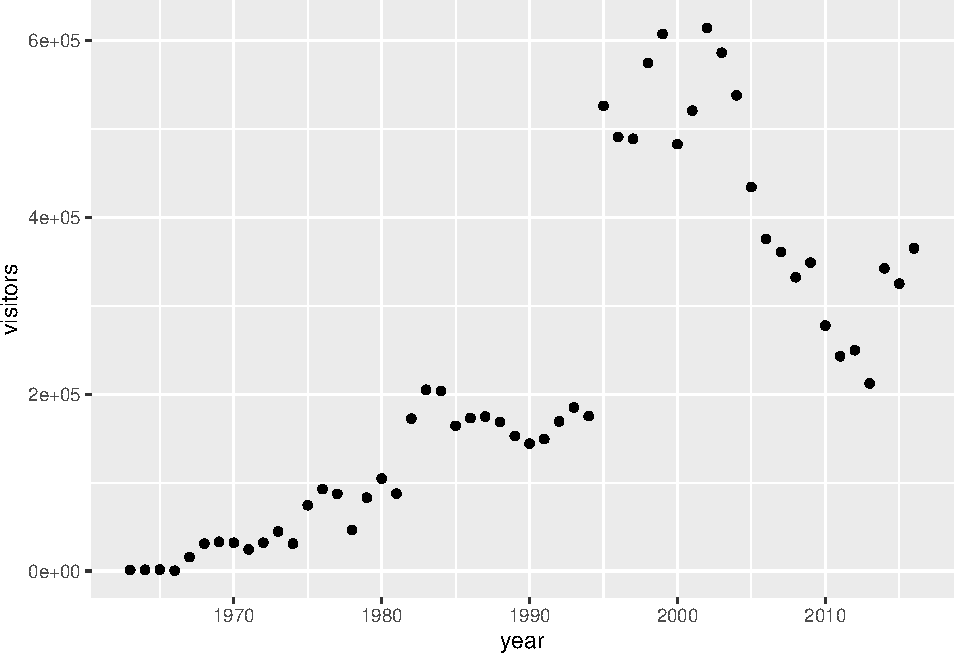
\includegraphics{R-for-Excel-Users_files/figure-latex/unnamed-chunk-31-1.pdf}

We could even do that for a column graph:

\begin{Shaded}
\begin{Highlighting}[]
\KeywordTok{ggplot}\NormalTok{(}\DataTypeTok{data =}\NormalTok{ ci_np, }\KeywordTok{aes}\NormalTok{(}\DataTypeTok{x =}\NormalTok{ year, }\DataTypeTok{y =}\NormalTok{ visitors)) }\OperatorTok{+}
\StringTok{  }\KeywordTok{geom_col}\NormalTok{()}
\end{Highlighting}
\end{Shaded}

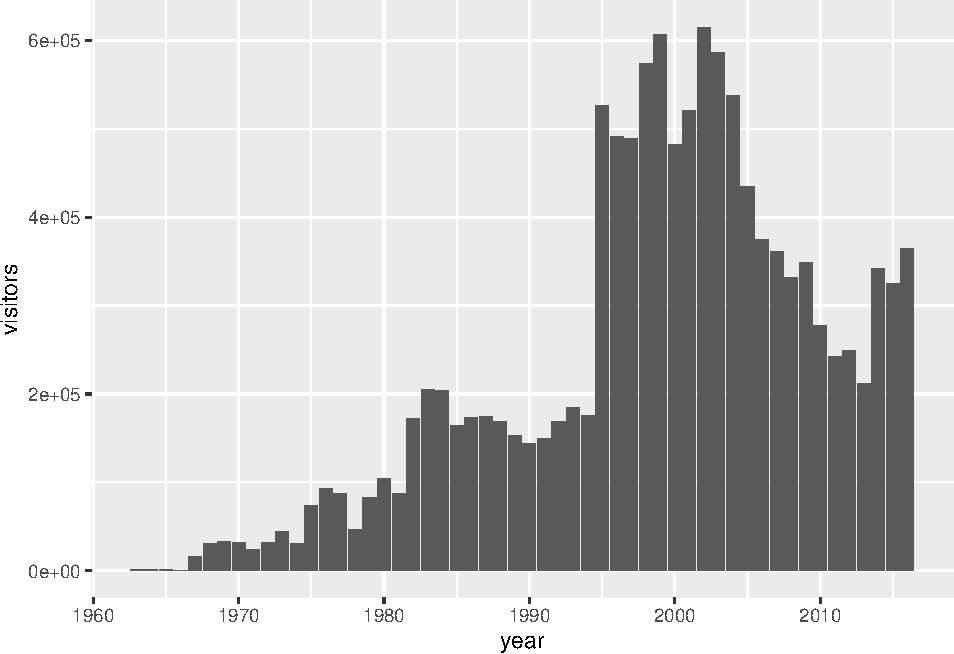
\includegraphics{R-for-Excel-Users_files/figure-latex/unnamed-chunk-32-1.pdf}

Or an area plot\ldots{}

\begin{Shaded}
\begin{Highlighting}[]
\KeywordTok{ggplot}\NormalTok{(}\DataTypeTok{data =}\NormalTok{ ci_np, }\KeywordTok{aes}\NormalTok{(}\DataTypeTok{x =}\NormalTok{ year, }\DataTypeTok{y =}\NormalTok{ visitors)) }\OperatorTok{+}
\StringTok{  }\KeywordTok{geom_area}\NormalTok{()}
\end{Highlighting}
\end{Shaded}

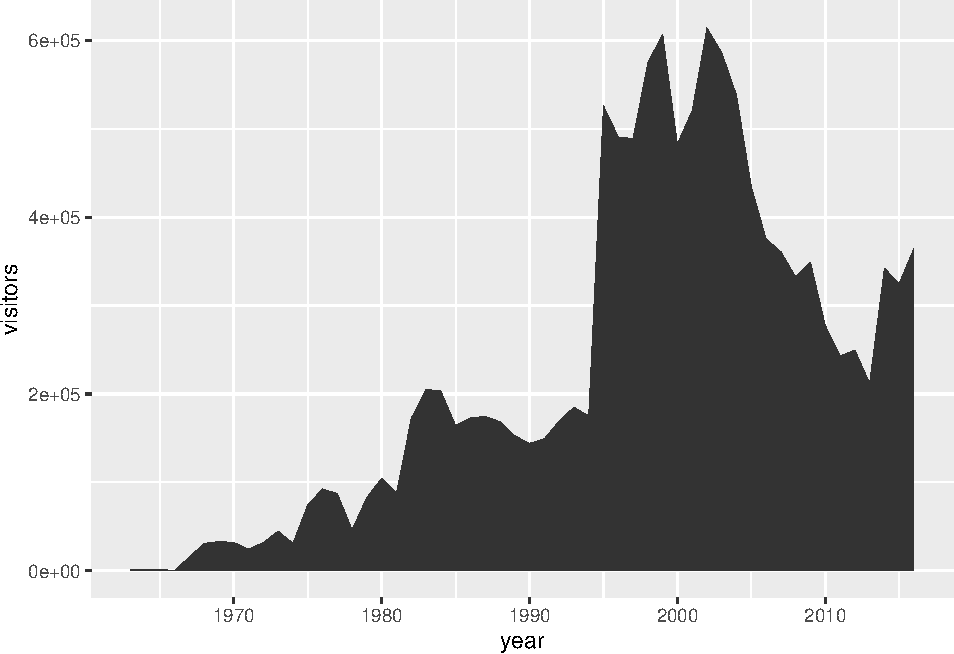
\includegraphics{R-for-Excel-Users_files/figure-latex/unnamed-chunk-33-1.pdf}

We can see that updating to different \texttt{geom\_*} types is quick, so long as the types of graphs we're switching between are compatible.

The data are there, now let's do some data viz customization.

\hypertarget{intro-to-customizing-ggplot-graphs}{%
\section{\texorpdfstring{Intro to customizing \texttt{ggplot} graphs}{Intro to customizing ggplot graphs}}\label{intro-to-customizing-ggplot-graphs}}

First, we'll customize some aesthetics (e.g.~colors, styles, axis labels, etc.) of our graphs based on non-variable values.

\begin{quote}
We can change the aesthetics of elements in a ggplot graph by adding arguments within the layer where that element is created.
\end{quote}

Some common arguments we'll use first are:

\begin{itemize}
\tightlist
\item
  \texttt{color\ =} or \texttt{colour\ =}: update point or line colors
\item
  \texttt{fill\ =}: update fill color for objects with areas
\item
  \texttt{linetype\ =}: update the line type (dashed, long dash, etc.)
\item
  \texttt{pch\ =}: update the point style
\item
  \texttt{size\ =}: update the element size (e.g.~of points or line thickness)
\item
  \texttt{alpha\ =}: update element opacity (1 = opaque, 0 = transparent)
\end{itemize}

Building on our first line graph, let's update the line color to ``purple'' and make the line type ``dashed'':

\begin{Shaded}
\begin{Highlighting}[]
\KeywordTok{ggplot}\NormalTok{(}\DataTypeTok{data =}\NormalTok{ ci_np, }\KeywordTok{aes}\NormalTok{(}\DataTypeTok{x =}\NormalTok{ year, }\DataTypeTok{y =}\NormalTok{ visitors)) }\OperatorTok{+}
\StringTok{  }\KeywordTok{geom_line}\NormalTok{(}
    \DataTypeTok{color =} \StringTok{"purple"}\NormalTok{,}
    \DataTypeTok{linetype =} \StringTok{"dashed"}
\NormalTok{  )}
\end{Highlighting}
\end{Shaded}

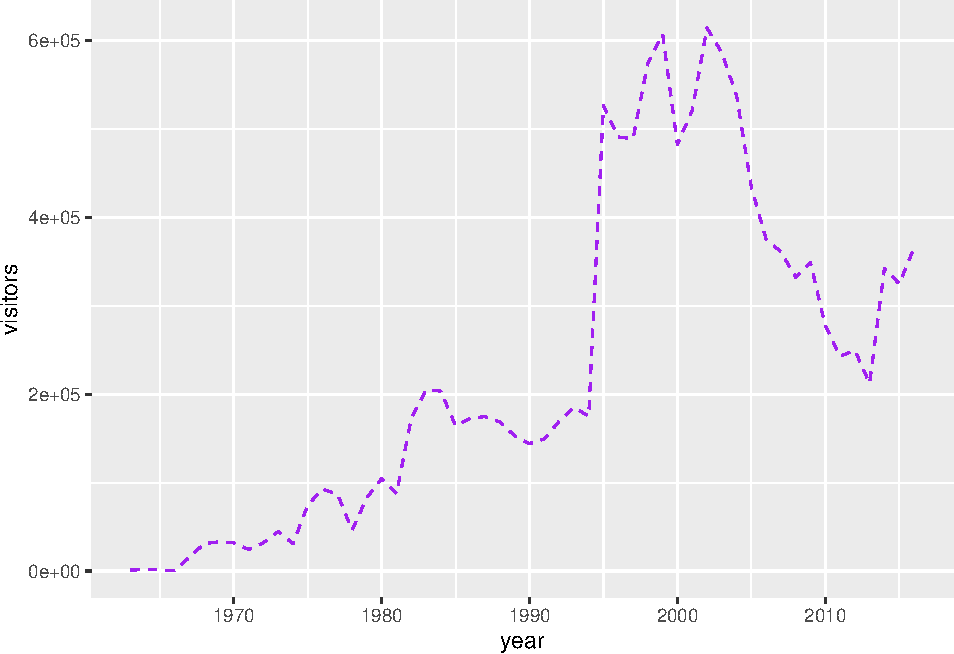
\includegraphics{R-for-Excel-Users_files/figure-latex/unnamed-chunk-34-1.pdf}

How do we know which color names ggplot will recognize? If you google ``R colors ggplot2'' you'll find a lot of good resources. Here's one: \href{http://sape.inf.usi.ch/quick-reference/ggplot2/colour}{SAPE ggplot2 colors quick reference guide}

Now let's update the point, style and size of points on our previous scatterplot graph using \texttt{color\ =}, \texttt{size\ =}, and \texttt{pch\ =} (see \texttt{?pch} for the different point styles, which can be further customized).

\begin{Shaded}
\begin{Highlighting}[]
\KeywordTok{ggplot}\NormalTok{(}\DataTypeTok{data =}\NormalTok{ ci_np, }\KeywordTok{aes}\NormalTok{(}\DataTypeTok{x =}\NormalTok{ year, }\DataTypeTok{y =}\NormalTok{ visitors)) }\OperatorTok{+}
\StringTok{  }\KeywordTok{geom_point}\NormalTok{(}\DataTypeTok{color =} \StringTok{"purple"}\NormalTok{,}
             \DataTypeTok{pch =} \DecValTok{17}\NormalTok{,}
             \DataTypeTok{size =} \DecValTok{4}\NormalTok{,}
             \DataTypeTok{alpha =} \FloatTok{0.5}\NormalTok{)}
\end{Highlighting}
\end{Shaded}

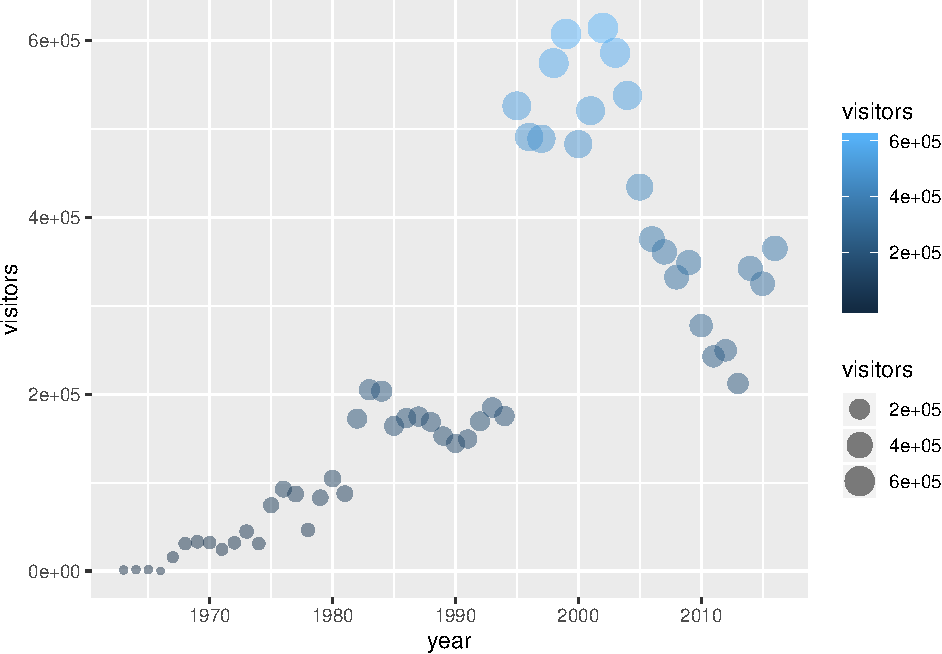
\includegraphics{R-for-Excel-Users_files/figure-latex/unnamed-chunk-35-1.pdf}

\hypertarget{activity-customize-your-own-ggplot-graph}{%
\subsection{Activity: customize your own ggplot graph}\label{activity-customize-your-own-ggplot-graph}}

Update one of the example graphs you created above to customize \textbf{at least} an element color and size!

\hypertarget{mapping-variables-onto-aesthetics}{%
\section{Mapping variables onto aesthetics}\label{mapping-variables-onto-aesthetics}}

In the examples above, we have customized aesthetics based on constants that we input as arguments (e.g., the color / style / size isn't changing based on a variable characteristic or value). Sometimes, however, we \textbf{do} want the aesthetics of a graph to depend on a variable. To do that, we'll \textbf{map variables onto graph aesthetics}, meaning we'll change how an element on the graph looks based on a variable characteristic (usually, character or value).

\begin{quote}
When we want to customize a graph element based on a variable's characteristic or value, add the argument within \texttt{aes()} in the appropriate \texttt{geom\_*()} layer
\end{quote}

In short, if updating aesthetics based on a variable, make sure to put that argument inside of \texttt{aes()}.

\textbf{Example:} Create a ggplot scatterplot graph where the \textbf{size} and \textbf{color} of the points change based on the \textbf{number of visitors}, and make all points the same level of opacity (\texttt{alpha\ =\ 0.5}). Notice the \texttt{aes()} around the \texttt{size\ =} and \texttt{color\ =} arguments.

Also: this is overmapped and unnecessary. Avoid excessive / overcomplicated aesthetic mapping in data visualization.

\begin{Shaded}
\begin{Highlighting}[]
\KeywordTok{ggplot}\NormalTok{(}\DataTypeTok{data =}\NormalTok{ ci_np, }\KeywordTok{aes}\NormalTok{(}\DataTypeTok{x =}\NormalTok{ year, }\DataTypeTok{y =}\NormalTok{ visitors)) }\OperatorTok{+}
\StringTok{  }\KeywordTok{geom_point}\NormalTok{(}
    \KeywordTok{aes}\NormalTok{(}\DataTypeTok{size =}\NormalTok{ visitors,}
        \DataTypeTok{color =}\NormalTok{ visitors),}
    \DataTypeTok{alpha =} \FloatTok{0.5}
\NormalTok{  )}
\end{Highlighting}
\end{Shaded}

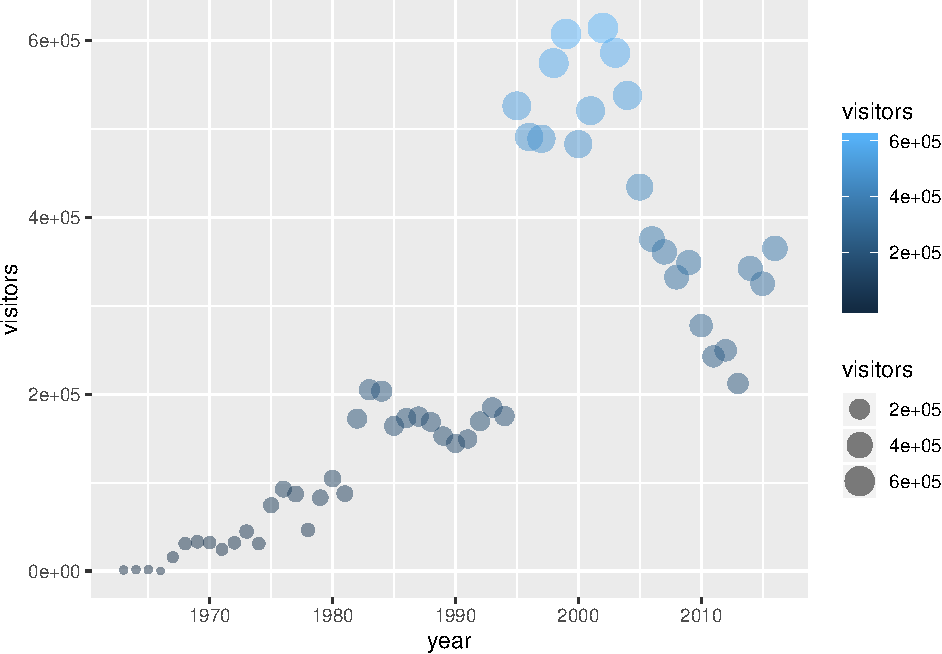
\includegraphics{R-for-Excel-Users_files/figure-latex/unnamed-chunk-36-1.pdf}

In the example above, notice that the two arguments that \textbf{do} depend on variables are within \texttt{aes()}, but since \texttt{alpha\ =\ 0.5} doesn't depend on a variable then it is \emph{outside the \texttt{aes()} but still within the \texttt{geom\_point()} layer}.

\hypertarget{activity-map-variables-onto-graph-aesthetics}{%
\subsection{Activity: map variables onto graph aesthetics}\label{activity-map-variables-onto-graph-aesthetics}}

Create a column plot of Channel Islands National Park visitation over time, where the \textbf{fill color} (argument: \texttt{fill\ =}) changes based on the number of \textbf{visitors}.

\begin{Shaded}
\begin{Highlighting}[]
\KeywordTok{ggplot}\NormalTok{(}\DataTypeTok{data =}\NormalTok{ ci_np, }\KeywordTok{aes}\NormalTok{(}\DataTypeTok{x =}\NormalTok{ year, }\DataTypeTok{y =}\NormalTok{ visitors)) }\OperatorTok{+}
\StringTok{  }\KeywordTok{geom_col}\NormalTok{(}\KeywordTok{aes}\NormalTok{(}\DataTypeTok{fill =}\NormalTok{ visitors))}
\end{Highlighting}
\end{Shaded}

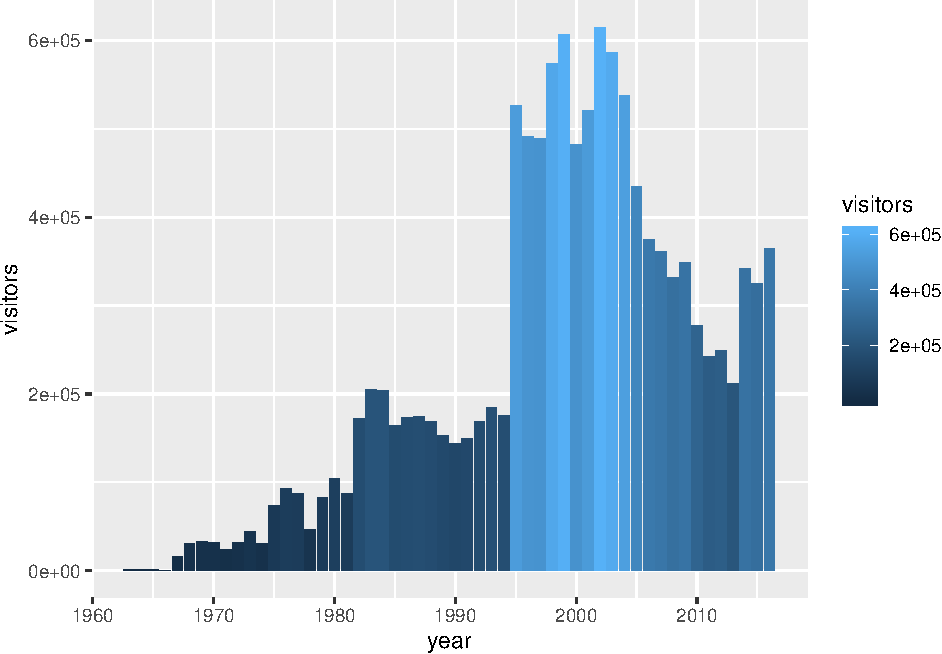
\includegraphics{R-for-Excel-Users_files/figure-latex/unnamed-chunk-37-1.pdf}

\textbf{Sync your project with your GitHub repo.}

\hypertarget{ggplot2-complete-themes}{%
\section{ggplot2 complete themes}\label{ggplot2-complete-themes}}

While every element of a ggplot graph is manually customizable, there are also built-in themes (\texttt{theme\_*()}) that you can add to your ggplot code to make some major headway before making smaller tweaks manually.

Here are a few to try today (but also notice all the options that appear as we start typing \texttt{theme\_} into our ggplot graph code!):

\begin{itemize}
\tightlist
\item
  \texttt{theme\_light()}
\item
  \texttt{theme\_minimal()}
\item
  \texttt{theme\_bw()}
\end{itemize}

Here, let's update our previous graph with \texttt{theme\_minimal()}:

\begin{Shaded}
\begin{Highlighting}[]
\KeywordTok{ggplot}\NormalTok{(}\DataTypeTok{data =}\NormalTok{ ci_np, }\KeywordTok{aes}\NormalTok{(}\DataTypeTok{x =}\NormalTok{ year, }\DataTypeTok{y =}\NormalTok{ visitors)) }\OperatorTok{+}
\StringTok{  }\KeywordTok{geom_point}\NormalTok{(}
    \KeywordTok{aes}\NormalTok{(}\DataTypeTok{size =}\NormalTok{ visitors,}
        \DataTypeTok{color =}\NormalTok{ visitors),}
    \DataTypeTok{alpha =} \FloatTok{0.5}
\NormalTok{  ) }\OperatorTok{+}
\StringTok{  }\KeywordTok{theme_minimal}\NormalTok{()}
\end{Highlighting}
\end{Shaded}

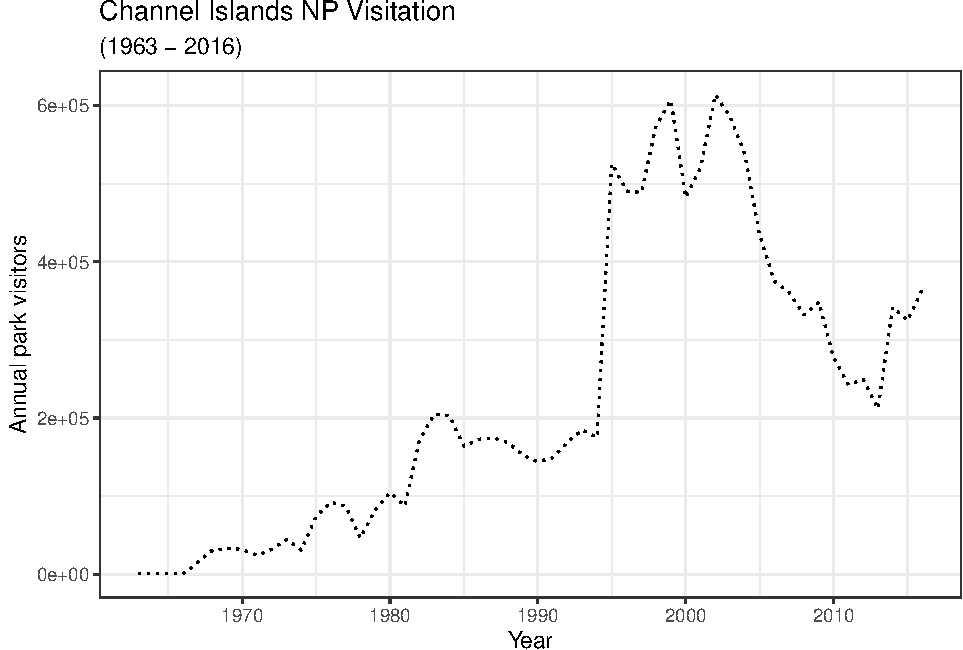
\includegraphics{R-for-Excel-Users_files/figure-latex/unnamed-chunk-38-1.pdf}

\hypertarget{updating-axis-labels-and-titles}{%
\section{Updating axis labels and titles}\label{updating-axis-labels-and-titles}}

Use \texttt{labs()} to update axis labels, and add a title and/or subtitle to your ggplot graph.

\begin{Shaded}
\begin{Highlighting}[]
\KeywordTok{ggplot}\NormalTok{(}\DataTypeTok{data =}\NormalTok{ ci_np, }\KeywordTok{aes}\NormalTok{(}\DataTypeTok{x =}\NormalTok{ year, }\DataTypeTok{y =}\NormalTok{ visitors)) }\OperatorTok{+}
\StringTok{  }\KeywordTok{geom_line}\NormalTok{(}\DataTypeTok{linetype =} \StringTok{"dotted"}\NormalTok{) }\OperatorTok{+}
\StringTok{  }\KeywordTok{theme_bw}\NormalTok{() }\OperatorTok{+}
\StringTok{  }\KeywordTok{labs}\NormalTok{(}
    \DataTypeTok{x =} \StringTok{"Year"}\NormalTok{,}
    \DataTypeTok{y =} \StringTok{"Annual park visitors"}\NormalTok{,}
    \DataTypeTok{title =} \StringTok{"Channel Islands NP Visitation"}\NormalTok{,}
    \DataTypeTok{subtitle =} \StringTok{"(1963 - 2016)"}
\NormalTok{  )}
\end{Highlighting}
\end{Shaded}

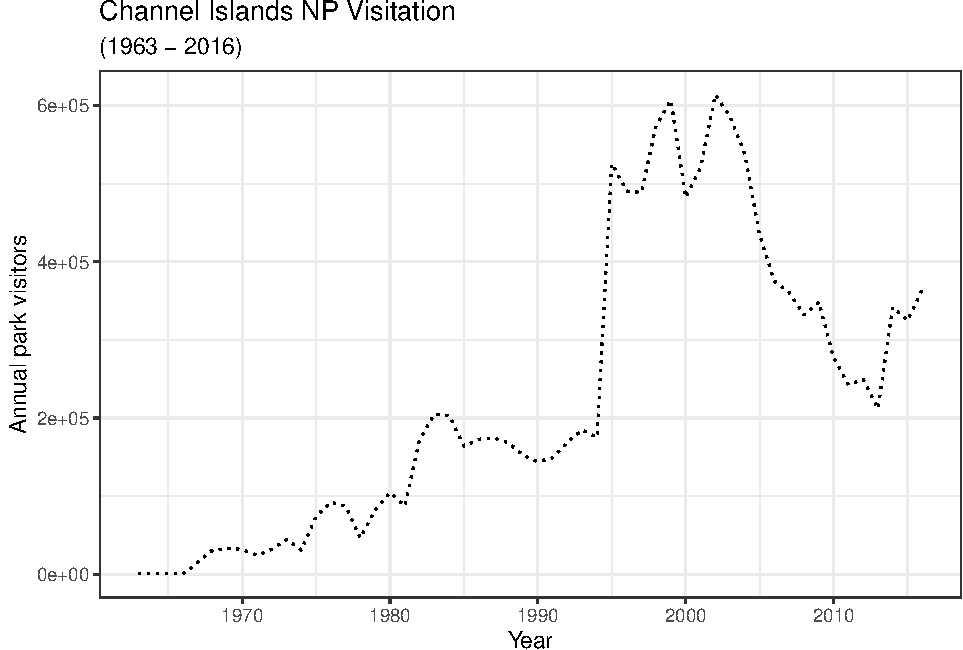
\includegraphics{R-for-Excel-Users_files/figure-latex/unnamed-chunk-39-1.pdf}

\textbf{Note}: If you want to update the formatting of axis values (for example, to convert to comma format instead of scientific format above), you can use the \texttt{scales} package options (see more from the \href{http://www.cookbook-r.com/Graphs/Axes_(ggplot2)/}{R Cookbook}).

\hypertarget{combining-compatible-geoms}{%
\section{Combining compatible geoms}\label{combining-compatible-geoms}}

As long as the geoms are compatible, we can layer them on top of one another to further customize a graph.

For example, adding points to a line graph:

\begin{Shaded}
\begin{Highlighting}[]
\KeywordTok{ggplot}\NormalTok{(}\DataTypeTok{data =}\NormalTok{ ci_np, }\KeywordTok{aes}\NormalTok{(}\DataTypeTok{x =}\NormalTok{ year, }\DataTypeTok{y =}\NormalTok{ visitors)) }\OperatorTok{+}
\StringTok{  }\KeywordTok{geom_line}\NormalTok{(}\DataTypeTok{color =} \StringTok{"purple"}\NormalTok{) }\OperatorTok{+}
\StringTok{  }\KeywordTok{geom_point}\NormalTok{(}\DataTypeTok{color =} \StringTok{"magenta"}\NormalTok{,}
             \KeywordTok{aes}\NormalTok{(}\DataTypeTok{size =}\NormalTok{ year))}
\end{Highlighting}
\end{Shaded}

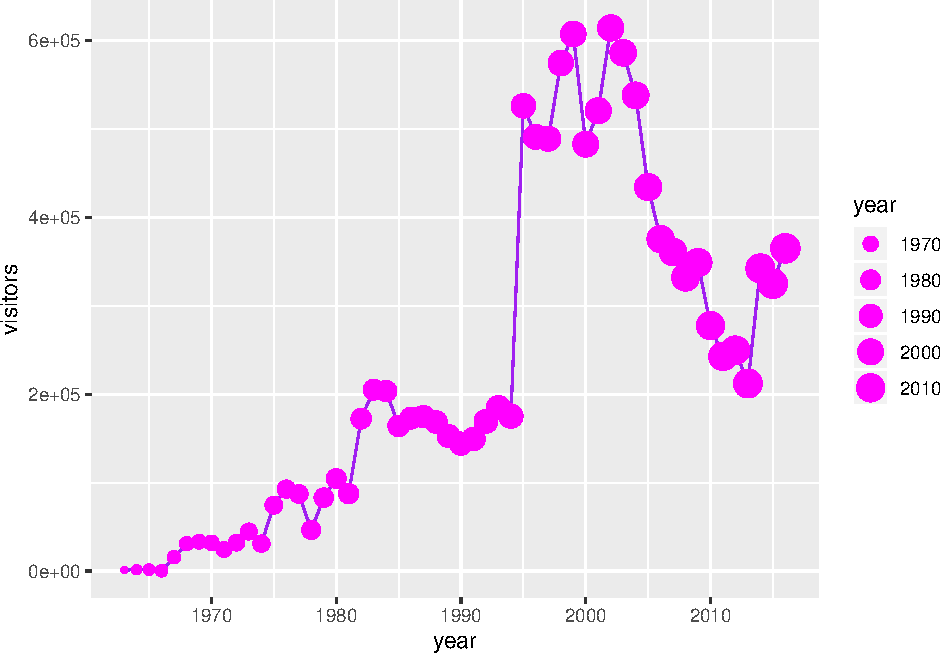
\includegraphics{R-for-Excel-Users_files/figure-latex/unnamed-chunk-40-1.pdf}

Or, combine a column and line graph (not sure why you'd want to do this, but you can):

\begin{Shaded}
\begin{Highlighting}[]
\KeywordTok{ggplot}\NormalTok{(}\DataTypeTok{data =}\NormalTok{ ci_np, }\KeywordTok{aes}\NormalTok{(}\DataTypeTok{x =}\NormalTok{ year, }\DataTypeTok{y =}\NormalTok{ visitors)) }\OperatorTok{+}
\StringTok{  }\KeywordTok{geom_col}\NormalTok{(}\DataTypeTok{fill =} \StringTok{"orange"}\NormalTok{,}
           \DataTypeTok{color =} \StringTok{"purple"}\NormalTok{) }\OperatorTok{+}
\StringTok{  }\KeywordTok{geom_line}\NormalTok{()}
\end{Highlighting}
\end{Shaded}

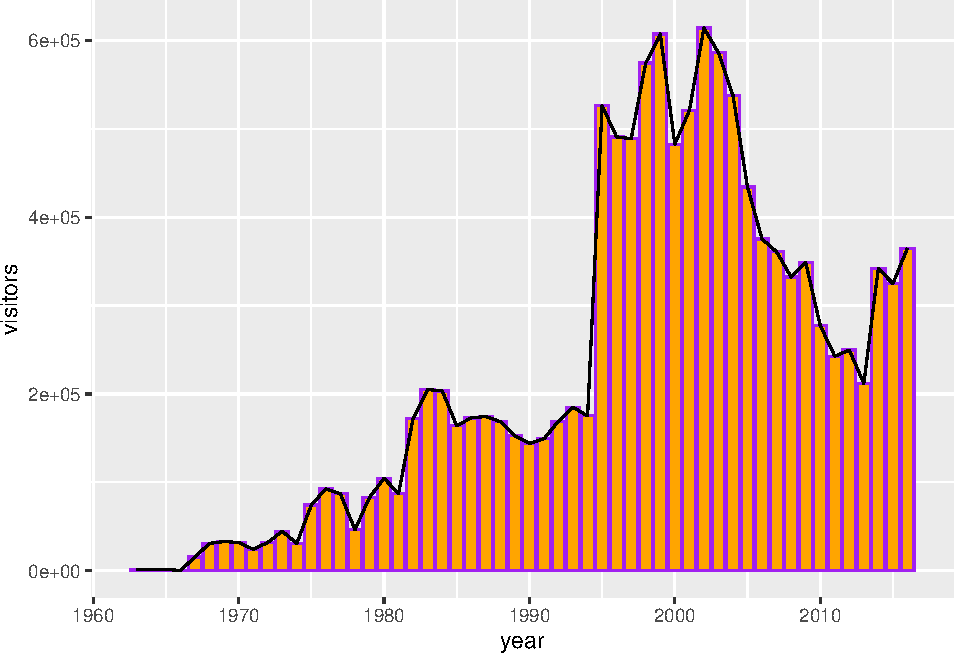
\includegraphics{R-for-Excel-Users_files/figure-latex/unnamed-chunk-41-1.pdf}

\hypertarget{multi-series-ggplot-graphs}{%
\section{Multi-series ggplot graphs}\label{multi-series-ggplot-graphs}}

In the examples above, we only had a single series - visitation at Channel Islands National Park. Often we'll want to visualize multiple series. For example, from the \texttt{ca\_np} object we have stored, we might want to plot visitation for \emph{all} California National Parks.

To do that, we need to add an aesthetic that lets \texttt{ggplot} know how things are going to be grouped. A demonstration of why that's important - what happens if we \emph{don't} let ggplot know how to group things?

\begin{Shaded}
\begin{Highlighting}[]
\KeywordTok{ggplot}\NormalTok{(}\DataTypeTok{data =}\NormalTok{ ca_np, }\KeywordTok{aes}\NormalTok{(}\DataTypeTok{x =}\NormalTok{ year, }\DataTypeTok{y =}\NormalTok{ visitors)) }\OperatorTok{+}
\StringTok{  }\KeywordTok{geom_line}\NormalTok{()}
\end{Highlighting}
\end{Shaded}

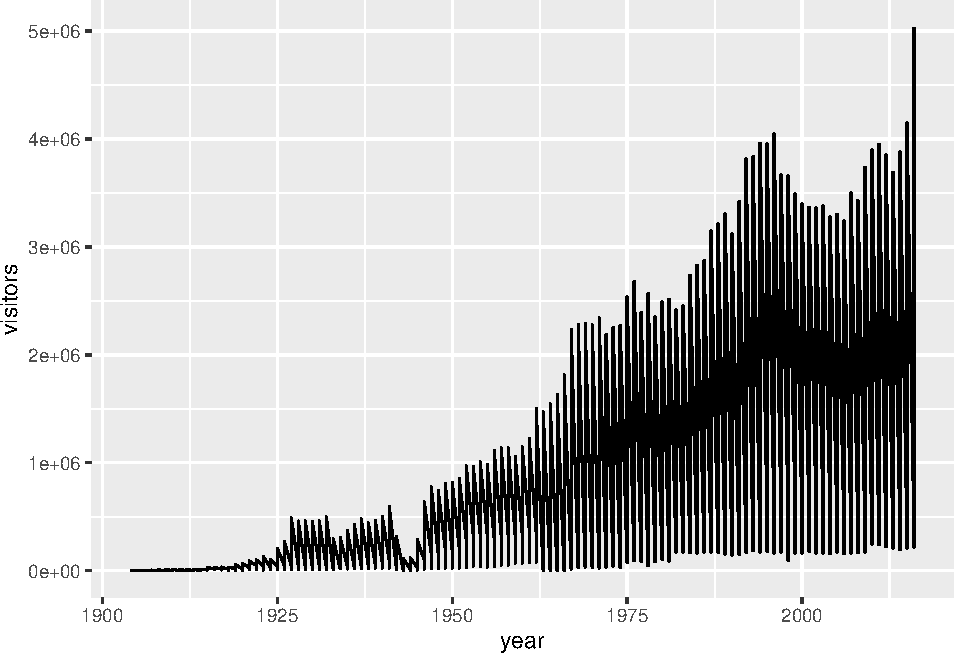
\includegraphics{R-for-Excel-Users_files/figure-latex/unnamed-chunk-42-1.pdf}

Well that's definitely a mess, and it's because ggplot has no idea that these \textbf{should be different series based on the different parks that appear in the `park\_name' column}.

We can make sure R does know by updating an aesthetic based on \emph{park\_name}:

\begin{Shaded}
\begin{Highlighting}[]
\KeywordTok{ggplot}\NormalTok{(}\DataTypeTok{data =}\NormalTok{ ca_np, }\KeywordTok{aes}\NormalTok{(}\DataTypeTok{x =}\NormalTok{ year, }\DataTypeTok{y =}\NormalTok{ visitors, }\DataTypeTok{color =}\NormalTok{ park_name)) }\OperatorTok{+}
\StringTok{  }\KeywordTok{geom_line}\NormalTok{()}
\end{Highlighting}
\end{Shaded}

\includegraphics{R-for-Excel-Users_files/figure-latex/unnamed-chunk-43-1.pdf}

\textbf{Note}: You could also add that aesthetic (\texttt{color\ =\ park\_name}) in the \texttt{geom\_line()} layer, instead of in the topmost \texttt{ggplot()} layer.

\hypertarget{faceting-ggplot-graphs}{%
\section{Faceting ggplot graphs}\label{faceting-ggplot-graphs}}

When we facet graphs, we split them up into multiple plotting panels, where each panel contains a subset of the data. In our case, we'll split the graph above into different panels, each containing visitation data for a single park.

Also notice that any general theme changes made will be applied to \emph{all} of the graphs.

\begin{Shaded}
\begin{Highlighting}[]
\KeywordTok{ggplot}\NormalTok{(}\DataTypeTok{data =}\NormalTok{ ca_np, }\KeywordTok{aes}\NormalTok{(}\DataTypeTok{x =}\NormalTok{ year, }\DataTypeTok{y =}\NormalTok{ visitors, }\DataTypeTok{color =}\NormalTok{ park_name)) }\OperatorTok{+}
\StringTok{  }\KeywordTok{geom_line}\NormalTok{(}\DataTypeTok{show.legend =} \OtherTok{FALSE}\NormalTok{) }\OperatorTok{+}
\StringTok{  }\KeywordTok{theme_light}\NormalTok{() }\OperatorTok{+}\StringTok{ }
\StringTok{  }\KeywordTok{labs}\NormalTok{(}\DataTypeTok{x =} \StringTok{"year"}\NormalTok{, }\DataTypeTok{y =} \StringTok{"annual visitors"}\NormalTok{) }\OperatorTok{+}
\StringTok{  }\KeywordTok{facet_wrap}\NormalTok{(}\OperatorTok{~}\StringTok{ }\NormalTok{park_name)}
\end{Highlighting}
\end{Shaded}

\includegraphics{R-for-Excel-Users_files/figure-latex/unnamed-chunk-44-1.pdf}

\hypertarget{exporting-a-ggplot-graph-with-ggsave}{%
\section{\texorpdfstring{Exporting a ggplot graph with \texttt{ggsave()}}{Exporting a ggplot graph with ggsave()}}\label{exporting-a-ggplot-graph-with-ggsave}}

If we want our graph to appear in a knitted html, then we don't need to do anything else. But often we'll need a saved image file, of specific size and resolution, to share or for publication.

\texttt{ggsave()} will export the \emph{most recently run} ggplot graph by default (\texttt{plot\ =\ last\_plot()}), unless you give it the name of a different saved ggplot object. Some common arguments for \texttt{ggsave()}:

\begin{itemize}
\tightlist
\item
  \texttt{width\ =}: set exported image width (default inches)
\item
  \texttt{height\ =}: set exported image height (default height)
\item
  \texttt{dpi\ =}: set dpi (dots per inch)
\end{itemize}

So to export the faceted graph above at 180 dpi, width a width of 8" and a height of 7", we can use:

\begin{Shaded}
\begin{Highlighting}[]
\KeywordTok{ggsave}\NormalTok{(}\KeywordTok{here}\NormalTok{(}\StringTok{"figures"}\NormalTok{, }\StringTok{"np_graph.jpg"}\NormalTok{), }\DataTypeTok{dpi =} \DecValTok{180}\NormalTok{, }\DataTypeTok{width =} \DecValTok{8}\NormalTok{, }\DataTypeTok{height =} \DecValTok{7}\NormalTok{)}
\end{Highlighting}
\end{Shaded}

Notice that a .jpg image of that name and size is now stored in your project working directory. You can change the type of exported image, too (e.g.~pdf, tiff, eps, png, mmp, svg).

\hypertarget{one-final-graph-example-jitter-and-boxplots}{%
\subsection{One final graph example: jitter and boxplots}\label{one-final-graph-example-jitter-and-boxplots}}

For the record: this is not a good option for showing the visitation data because values are not independent observations of a random variable. But, for the purposes of showing a graph, we'll use visitation as our continuous measured variable in a jitter + boxplot anyway.

\begin{Shaded}
\begin{Highlighting}[]
\KeywordTok{ggplot}\NormalTok{(}\DataTypeTok{data =}\NormalTok{ ca_np, }\KeywordTok{aes}\NormalTok{(}\DataTypeTok{x =}\NormalTok{ park_name, }\DataTypeTok{y =}\NormalTok{ visitors)) }\OperatorTok{+}
\StringTok{  }\KeywordTok{geom_jitter}\NormalTok{(}\DataTypeTok{alpha =} \FloatTok{0.5}\NormalTok{,}
              \DataTypeTok{color =} \StringTok{"gray60"}\NormalTok{,}
              \DataTypeTok{width =} \FloatTok{0.2}\NormalTok{,}
              \DataTypeTok{size =} \DecValTok{1}\NormalTok{) }\OperatorTok{+}
\StringTok{  }\KeywordTok{geom_boxplot}\NormalTok{(}\DataTypeTok{fill =} \OtherTok{NA}\NormalTok{,}
               \DataTypeTok{color =} \StringTok{"black"}\NormalTok{,}
               \DataTypeTok{outlier.color =} \OtherTok{NA}\NormalTok{) }\OperatorTok{+}
\StringTok{  }\KeywordTok{coord_flip}\NormalTok{() }\OperatorTok{+}
\StringTok{  }\KeywordTok{theme_minimal}\NormalTok{()}
\end{Highlighting}
\end{Shaded}

\includegraphics{R-for-Excel-Users_files/figure-latex/unnamed-chunk-47-1.pdf}

\textbf{Sync your project with your GitHub repo.}

\hypertarget{end-ggplot-session}{%
\section{\texorpdfstring{End \texttt{ggplot} session}{End ggplot session}}\label{end-ggplot-session}}

\hypertarget{pivot}{%
\chapter{\texorpdfstring{\texttt{dplyr} and Pivot Tables}{dplyr and Pivot Tables}}\label{pivot}}

\hypertarget{summary-3}{%
\section{Summary}\label{summary-3}}

Pivot tables are powerful tools in Excel for summarizing data in different ways. We will create these tables using the \texttt{group\_by} and \texttt{summarize} functions from the \texttt{dplyr} package (part of the Tidyverse). We will also learn how to format tables and practice creating a reproducible report using RMarkdown and sharing it with GitHub.

\hypertarget{objectives-3}{%
\section{Objectives}\label{objectives-3}}

In R, we can use dplyr for pivot tables by using 2 main verbs in combination: \texttt{group\_by} and \texttt{summarize}. We will also continue to emphasize reproducibility in all our analyses.

\begin{itemize}
\tightlist
\item
  Discuss pivot tables in Excel
\item
  Introduce \texttt{group\_by()\ \%\textgreater{}\%\ summarize()} from the \texttt{dplyr} package
\item
  Practice our reproducible workflow with RMarkdown and GitHub
\end{itemize}

\hypertarget{resources-4}{%
\section{Resources}\label{resources-4}}

\begin{itemize}
\tightlist
\item
  \href{https://dplyr.tidyverse.org/}{dplyr.tidyverse.org}
\item
  \href{https://r4ds.had.co.nz/transform.html}{R for Data Science: Transform Chapter}
\item
  \href{https://youtu.be/g530cnFfk8Y}{Intro to Pivot Tables I-III} by Excel Campus (YouTube)
\end{itemize}

\hypertarget{pivot-table-overview}{%
\section{Pivot table overview}\label{pivot-table-overview}}

\href{https://en.wikipedia.org/wiki/Pivot_table}{Wikipedia describes a pivot table} as a ``table of statistics that summarizes the data of a more extensive table\ldots{}This summary might include sums, averages, or other statistics, which the pivot table groups together in a meaningful way.'' Fun fact: it also says that ``Although pivot table is a generic term, Microsoft trademarked PivotTable in the United States in 1994.''

Pivot tables are a really powerful tool for summarizing data, and we can have similar functionality in R --- as well as nicely automating and reporting these tables. We will learn about this using data about lobsters and will go back and forth between R and Excel as we learn.

Let's start off in R, and have a look at the data.

\hypertarget{rmarkdown-setup}{%
\section{RMarkdown setup}\label{rmarkdown-setup}}

Let's start a new RMarkdown file in our repo, at the top-level (where it will be created by default in our Project). I'll call mine \texttt{pivot\_lobsters.Rmd}.

In the setup chunk, let's attach our libraries and read in our lobster data. In addition to the \texttt{tidyverse} package we will also use the \texttt{skimr} package. You will have to install it, but don't want it to be installed every time you write your code. The following is a nice convention for having the install instructions available (on the same line) as the \texttt{library()} call.

\begin{Shaded}
\begin{Highlighting}[]
\CommentTok{## attach libraries}
\KeywordTok{library}\NormalTok{(tidyverse)}
\KeywordTok{library}\NormalTok{(readxl)}
\KeywordTok{library}\NormalTok{(here)}
\KeywordTok{library}\NormalTok{(skimr) }\CommentTok{# install.packages('skimr')}

\CommentTok{## read in data}
\NormalTok{lobsters <-}\StringTok{ }\KeywordTok{read_xlsx}\NormalTok{(}\KeywordTok{here}\NormalTok{(}\StringTok{"data/lobsters.xlsx"}\NormalTok{))}
\end{Highlighting}
\end{Shaded}

Let's add a code chunk and explore the data in a few ways.

\begin{Shaded}
\begin{Highlighting}[]
\CommentTok{# explore data}
\KeywordTok{head}\NormalTok{(lobsters) }\CommentTok{# year and month as well as a column for date}
\end{Highlighting}
\end{Shaded}

\begin{verbatim}
## # A tibble: 6 x 7
##    year month date    site  transect replicate size_mm
##   <dbl> <dbl> <chr>   <chr>    <dbl> <chr>       <dbl>
## 1  2012     8 8/20/12 ivee         3 A              70
## 2  2012     8 8/20/12 ivee         3 B              60
## 3  2012     8 8/20/12 ivee         3 B              65
## 4  2012     8 8/20/12 ivee         3 B              70
## 5  2012     8 8/20/12 ivee         3 B              85
## 6  2012     8 8/20/12 ivee         3 C              60
\end{verbatim}

\texttt{head()} gives us a look at the first rows of the data (6 by default). I like this because I can see the column names and get a sense of the shape of the data. I can also see the class of each column (double or character)

In this data set, every row is a unique observation. This is called ``uncounted'' data; you'll see there is no row for how many lobsters were seen because each row is an observation, or an ``n of 1''.

\begin{Shaded}
\begin{Highlighting}[]
\CommentTok{# explore data}
\KeywordTok{summary}\NormalTok{(lobsters) }
\end{Highlighting}
\end{Shaded}

\texttt{summary} gives us summary statistics for each variable (column). I like this for numeric columns, but it doesn't give a lot of useful information for non-numeric data. To have a look there I like using the skimr package:

\begin{Shaded}
\begin{Highlighting}[]
\CommentTok{# explore data}
\NormalTok{skimr}\OperatorTok{::}\KeywordTok{skim}\NormalTok{(lobsters) }
\end{Highlighting}
\end{Shaded}

This \texttt{skimr::} notation is a reminder to me that \texttt{skim} is from the \texttt{skimr} package. It is a nice convention: it's a reminder to others (especially you!).

\texttt{skim} lets us look more at each variable. I particularly like looking at missing data. There are 6 missing values in the \texttt{size\_mm} variable.

We can also make a quick plot to have a look at these data, and use our new ggplot2 skills. Let's make a bar chart by year for each site

\begin{Shaded}
\begin{Highlighting}[]
\KeywordTok{ggplot}\NormalTok{(lobsters, }\KeywordTok{aes}\NormalTok{(}\DataTypeTok{x =}\NormalTok{ year)) }\OperatorTok{+}
\StringTok{  }\KeywordTok{geom_bar}\NormalTok{() }\OperatorTok{+}
\StringTok{  }\KeywordTok{facet_wrap}\NormalTok{(}\OperatorTok{~}\NormalTok{site)}
\end{Highlighting}
\end{Shaded}

\includegraphics{R-for-Excel-Users_files/figure-latex/plot-lobsters-1.pdf}

(geom\_bar() counts things and geom\_col() is for values within the data (mean))

\hypertarget{our-task}{%
\subsection{Our task}\label{our-task}}

So this is all great to get a quick look. But what if we needed to report to someone about how the average size of lobsters has changed over time across sites?

To answer this we need to do a pivot table in Excel, or data wrangling in R.

Let's start by having a quick look at what pivot tables can do in Excel.

\hypertarget{pivot-table-demo}{%
\section{Pivot table demo}\label{pivot-table-demo}}

Let's make a pivot table with our lobster data.

Let's start off with how many lobsters were counted each year. I want a count of rows by year.

So to do this in Excel we would initiate the Pivot Table Process:

\includegraphics[width=0.6\linewidth]{img/pivot-table-menu}

And it will do its best to find the data I would like to include in my Pivot Table (it can have difficulty with non-rectangular or ``non-tidy'' data), and suggest we make this in a new sheet:

\includegraphics[width=0.6\linewidth]{img/pivot-table-create}

And then we'll get a little wizard to help us create the Pivot Table.

\hypertarget{pivot-one-variable}{%
\subsection{pivot one variable}\label{pivot-one-variable}}

I want to summarize by year, so I drag ``year'' down into the ``Rows'' box, and to get the counts by year I actually drag the same variable, ``year'' into the ``Values'' box. And it will create a Pivot Table for me! But ``sum'' as the default summary statistic, so I can click the little ``I'' icon to change this to count.

\includegraphics[width=0.6\linewidth]{img/pivot-table-count-year}

A few things to note:

\begin{itemize}
\tightlist
\item
  The pivot table is separate entity from our data (it's on a different sheet); the original data has not been affected
\item
  The pivot table only shows the variables we requested; we don't see other columns (like date, month, or site).
\item
  Notice that in Excel we retain the overall totals for each site (in bold, on the same line with the site name). This is nice for communicating about data. But it can be problematic for further analyses, because it could be easy to take a total of this column and introduce errors.
\end{itemize}

So pivot tables are great because they summarize the data and keep the raw data raw --- they even promote good pratice because they by default ask you if you'd like to present the data in a new sheet rather than in the same sheet.

\hypertarget{pivot-two-variables}{%
\subsection{pivot two variables}\label{pivot-two-variables}}

We can also add site as a second variable by dragging it:

\includegraphics[width=0.6\linewidth]{img/pivot-table-count-year-site}

And then can reverse the order by dragging:

\includegraphics[width=0.6\linewidth]{img/pivot-table-count-site-year}

So in terms of our final interest of average size by site and year, we are on our way! I'm going to stop here because we want to be able to do this in R.

The power of R is in the automation, and in keeping that raw data truly raw.

Let's talk about how this looks like in R.

\hypertarget{group_by-summarize}{%
\section{\texorpdfstring{\texttt{group\_by()} \%\textgreater{}\% \texttt{summarize()}}{group\_by() \%\textgreater{}\% summarize()}}\label{group_by-summarize}}

In R, we can create the functionality of pivot tables by using 2 main \texttt{dplyr} verbs in combination: \texttt{group\_by} and \texttt{summarize}.

Say it with me: ``pivot tables are group\_by and then summarize''. And just like pivot tables, you have flexibility with how you are going to summarize. For example, we can calculate an average, or a total.

I think it's incredibly powerful to visualize what we are talking about with our data when do do these kinds of operations. It looks like this (from \href{http://www.rstudio.com/wp-content/uploads/2015/02/data-wrangling-cheatsheet.pdf}{RStudio's cheatsheet}; all cheatsheets available from \url{https://rstudio.com/resources/cheatsheets}):

\includegraphics[width=0.8\linewidth]{img/rstudio-cheatsheet-group_by_summarize}

When we were reporting by year or site, we were essentially modifying what we were grouping by (the different colors here in this figure.

Let's do this in R.

\hypertarget{group_by-one-variable}{%
\subsection{\texorpdfstring{\texttt{group\_by} one variable}{group\_by one variable}}\label{group_by-one-variable}}

Let's try this on our \texttt{lobsters} data, just like we did in Excel. We will count the the total number of lobster by year. In R vocabulary, we will group\_by year and then summarize by counting using \texttt{n()}, which is a function from \texttt{dplyr}. \texttt{n()} counts the number of times an observation shows up, and since this is uncounted data, this will count each row. We'll also use the pipe operator \texttt{\%\textgreater{}\%}, which you can read as ``and then''.

This to me reads: ``take the lobsters data and then group\_by year and then summarize by count in a new column called `count'\,''

\begin{Shaded}
\begin{Highlighting}[]
\NormalTok{lobsters }\OperatorTok
\StringTok{  }\KeywordTok{group_by}\NormalTok{(year) }\OperatorTok
\StringTok{  }\KeywordTok{summarize}\NormalTok{(}\DataTypeTok{count_by_year =} \KeywordTok{n}\NormalTok{())}
\end{Highlighting}
\end{Shaded}

\begin{verbatim}
## # A tibble: 7 x 2
##    year count_by_year
##   <dbl>         <int>
## 1  2012           231
## 2  2013           243
## 3  2014           510
## 4  2015          1100
## 5  2016           809
## 6  2017          1668
## 7  2018          1805
\end{verbatim}

Notice how together, \texttt{group\_by} and \texttt{summarize} minimize the amount of information we see. We also saw this with the pivot table. We lose the other columns that aren't involved here.

Question: What if you \emph{don't} group\_by first? Let's try it and discuss what's going on.

\begin{Shaded}
\begin{Highlighting}[]
\NormalTok{lobsters }\OperatorTok
\StringTok{  }\KeywordTok{summarize}\NormalTok{(}\DataTypeTok{count =}  \KeywordTok{n}\NormalTok{())}
\end{Highlighting}
\end{Shaded}

\begin{verbatim}
## # A tibble: 1 x 1
##   count
##   <int>
## 1  6366
\end{verbatim}

So if we don't \texttt{group\_by} first, we will get a single summary statistic (sum in this case) for the whole dataset.

Another question: what if we \emph{only} group\_by?

\begin{Shaded}
\begin{Highlighting}[]
\NormalTok{lobsters }\OperatorTok
\StringTok{  }\KeywordTok{group_by}\NormalTok{(year)}
\end{Highlighting}
\end{Shaded}

\begin{verbatim}
## # A tibble: 6,366 x 7
## # Groups:   year [7]
##     year month date    site  transect replicate size_mm
##    <dbl> <dbl> <chr>   <chr>    <dbl> <chr>       <dbl>
##  1  2012     8 8/20/12 ivee         3 A              70
##  2  2012     8 8/20/12 ivee         3 B              60
##  3  2012     8 8/20/12 ivee         3 B              65
##  4  2012     8 8/20/12 ivee         3 B              70
##  5  2012     8 8/20/12 ivee         3 B              85
##  6  2012     8 8/20/12 ivee         3 C              60
##  7  2012     8 8/20/12 ivee         3 C              65
##  8  2012     8 8/20/12 ivee         3 C              67
##  9  2012     8 8/20/12 ivee         3 D              70
## 10  2012     8 8/20/12 ivee         4 B              85
## # ... with 6,356 more rows
\end{verbatim}

\hypertarget{rstudio-viewer}{%
\subsection{RStudio Viewer}\label{rstudio-viewer}}

Let's now check the \texttt{lobsters} variable. We can do this by clicking on \texttt{lobsters} in the Environment pane in RStudio.

We see that we haven't changed any of our original data that was stored in this variable. (Just like how the pivot table didn't affect the raw data on the original sheet).

\begin{quote}
\textbf{\emph{Aside}}: You'll also see that when you click on the variable name in the Environment pane, \texttt{View(lobsters)} shows up in your Console. \texttt{View()} (capital V) is the R function to view any variable in the viewer. So this is something that you can write in your RMarkdown script, although RMarkdown will not be able to knit this view feature into the formatted document. So, if you want include \texttt{View()} in your RMarkdown document you will need to either comment it out \texttt{\#View()} or add \texttt{eval=FALSE} to the top of the code chunk so that the full line reads \texttt{\{r,\ eval=FALSE\}}.
\end{quote}

\hypertarget{group_by-multiple-variables}{%
\subsection{\texorpdfstring{\texttt{group\_by} multiple variables}{group\_by multiple variables}}\label{group_by-multiple-variables}}

Great. Now let's summarize by both year and site like we did in the pivot table. We are able to \texttt{group\_by} more than one variable. Let's do this together:

\begin{Shaded}
\begin{Highlighting}[]
\NormalTok{lobsters }\OperatorTok
\StringTok{  }\KeywordTok{group_by}\NormalTok{(site, year) }\OperatorTok
\StringTok{  }\KeywordTok{summarize}\NormalTok{(}\DataTypeTok{count_by_siteyear =}  \KeywordTok{n}\NormalTok{())}
\end{Highlighting}
\end{Shaded}

\begin{verbatim}
## # A tibble: 35 x 3
## # Groups:   site [5]
##    site   year count_by_siteyear
##    <chr> <dbl>             <int>
##  1 aque   2012                38
##  2 aque   2013                32
##  3 aque   2014               100
##  4 aque   2015                83
##  5 aque   2016                48
##  6 aque   2017                67
##  7 aque   2018                54
##  8 carp   2012                78
##  9 carp   2013                93
## 10 carp   2014                79
## # ... with 25 more rows
\end{verbatim}

text.

\hypertarget{summarize-multiple-variables}{%
\subsection{\texorpdfstring{\texttt{summarize} multiple variables}{summarize multiple variables}}\label{summarize-multiple-variables}}

We can summarize multiple variables at a time. So far we've done the count of lobster observations. Let's also do the mean and standard deviation. First let's use the \texttt{mean()} function to calculate the mean. We do this within the same summarize() function, but we can add a new line to make it easier to read. Notice how when you put your curser within the parenthesis and hit return, the indentation will automatically align.

\begin{Shaded}
\begin{Highlighting}[]
\NormalTok{lobsters }\OperatorTok
\StringTok{  }\KeywordTok{group_by}\NormalTok{(site, year) }\OperatorTok
\StringTok{  }\KeywordTok{summarize}\NormalTok{(}\DataTypeTok{count_by_siteyear =}  \KeywordTok{n}\NormalTok{(),}
            \DataTypeTok{mean_size_mm =} \KeywordTok{mean}\NormalTok{(size_mm))}
\end{Highlighting}
\end{Shaded}

\begin{verbatim}
## # A tibble: 35 x 4
## # Groups:   site [5]
##    site   year count_by_siteyear mean_size_mm
##    <chr> <dbl>             <int>        <dbl>
##  1 aque   2012                38         71  
##  2 aque   2013                32         72.1
##  3 aque   2014               100         76.9
##  4 aque   2015                83         68.5
##  5 aque   2016                48         68.7
##  6 aque   2017                67         73.9
##  7 aque   2018                54         71.7
##  8 carp   2012                78         74.4
##  9 carp   2013                93         76.6
## 10 carp   2014                79         NA  
## # ... with 25 more rows
\end{verbatim}

\begin{quote}
\textbf{\emph{Aside}} Command-I will properly indent selected lines.
\end{quote}

Great! But this will actually calculate some of the means as NA because one or more values in that year are NA. So we can pass an argument that says to remove NAs first before calculating the average. Let's do that, and then also calculate the standard deviation with the \texttt{sd()} function:

\begin{Shaded}
\begin{Highlighting}[]
\NormalTok{lobsters }\OperatorTok
\StringTok{  }\KeywordTok{group_by}\NormalTok{(site, year) }\OperatorTok
\StringTok{  }\KeywordTok{summarize}\NormalTok{(}\DataTypeTok{count_by_siteyear =}  \KeywordTok{n}\NormalTok{(), }
            \DataTypeTok{mean_size_mm =} \KeywordTok{mean}\NormalTok{(size_mm, }\DataTypeTok{na.rm=}\OtherTok{TRUE}\NormalTok{), }
            \DataTypeTok{sd_size_mm =} \KeywordTok{sd}\NormalTok{(size_mm, }\DataTypeTok{na.rm=}\OtherTok{TRUE}\NormalTok{))}
\end{Highlighting}
\end{Shaded}

\begin{verbatim}
## # A tibble: 35 x 5
## # Groups:   site [5]
##    site   year count_by_siteyear mean_size_mm sd_size_mm
##    <chr> <dbl>             <int>        <dbl>      <dbl>
##  1 aque   2012                38         71        10.2 
##  2 aque   2013                32         72.1      12.3 
##  3 aque   2014               100         76.9       9.32
##  4 aque   2015                83         68.5      12.6 
##  5 aque   2016                48         68.7      12.5 
##  6 aque   2017                67         73.9      11.9 
##  7 aque   2018                54         71.7       8.14
##  8 carp   2012                78         74.4      14.6 
##  9 carp   2013                93         76.6       8.71
## 10 carp   2014                79         79.1       8.57
## # ... with 25 more rows
\end{verbatim}

So we can make the equivalent of Excel's pivot table in R with \texttt{group\_by} and then \texttt{summarize}. But a powerful thing about R is that maybe we want this information to be used in further analyses. We can make this easier for ourselves by saving this as a variable. So let's add a variable assignment to that first line:

\begin{Shaded}
\begin{Highlighting}[]
\NormalTok{siteyear_summary <-}\StringTok{ }\NormalTok{lobsters }\OperatorTok
\StringTok{  }\KeywordTok{group_by}\NormalTok{(site, year) }\OperatorTok
\StringTok{  }\KeywordTok{summarize}\NormalTok{(}\DataTypeTok{count_by_siteyear =}  \KeywordTok{n}\NormalTok{(), }
            \DataTypeTok{mean_size_mm =} \KeywordTok{mean}\NormalTok{(size_mm, }\DataTypeTok{na.rm =} \OtherTok{TRUE}\NormalTok{), }
            \DataTypeTok{sd_size_mm =} \KeywordTok{sd}\NormalTok{(size_mm, }\DataTypeTok{na.rm =} \OtherTok{TRUE}\NormalTok{))}

\NormalTok{siteyear_summary}
\end{Highlighting}
\end{Shaded}

\begin{verbatim}
## # A tibble: 35 x 5
## # Groups:   site [5]
##    site   year count_by_siteyear mean_size_mm sd_size_mm
##    <chr> <dbl>             <int>        <dbl>      <dbl>
##  1 aque   2012                38         71        10.2 
##  2 aque   2013                32         72.1      12.3 
##  3 aque   2014               100         76.9       9.32
##  4 aque   2015                83         68.5      12.6 
##  5 aque   2016                48         68.7      12.5 
##  6 aque   2017                67         73.9      11.9 
##  7 aque   2018                54         71.7       8.14
##  8 carp   2012                78         74.4      14.6 
##  9 carp   2013                93         76.6       8.71
## 10 carp   2014                79         79.1       8.57
## # ... with 25 more rows
\end{verbatim}

\hypertarget{activity-2}{%
\subsection{Activity}\label{activity-2}}

\begin{enumerate}
\def\labelenumi{\arabic{enumi}.}
\tightlist
\item
  Calculate the median \texttt{size\_mm} (Hint: ?median) and
\item
  create and ggsave() a plot.
\end{enumerate}

Then, save, commit, and push your .Rmd, .html, and .png.

Solution (no peeking):

\begin{Shaded}
\begin{Highlighting}[]
\NormalTok{siteyear_summary <-}\StringTok{ }\NormalTok{lobsters }\OperatorTok
\StringTok{  }\KeywordTok{group_by}\NormalTok{(site, year) }\OperatorTok
\StringTok{  }\KeywordTok{summarize}\NormalTok{(}\DataTypeTok{count_by_siteyear =}  \KeywordTok{n}\NormalTok{(), }
            \DataTypeTok{mean_size_mm =} \KeywordTok{mean}\NormalTok{(size_mm, }\DataTypeTok{na.rm =} \OtherTok{TRUE}\NormalTok{), }
            \DataTypeTok{sd_size_mm =} \KeywordTok{sd}\NormalTok{(size_mm, }\DataTypeTok{na.rm =} \OtherTok{TRUE}\NormalTok{), }
            \DataTypeTok{median_size_mm =} \KeywordTok{median}\NormalTok{(size_mm, }\DataTypeTok{na.rm =} \OtherTok{TRUE}\NormalTok{))}

\NormalTok{siteyear_summary}

\CommentTok{## a ggplot option:}
\KeywordTok{ggplot}\NormalTok{(}\DataTypeTok{data =}\NormalTok{ siteyear_summary, }\KeywordTok{aes}\NormalTok{(}\DataTypeTok{x =}\NormalTok{ year, }\DataTypeTok{y =}\NormalTok{ median_size_mm, }\DataTypeTok{color =}\NormalTok{ site)) }\OperatorTok{+}
\StringTok{  }\KeywordTok{geom_line}\NormalTok{() }
\KeywordTok{ggsave}\NormalTok{(}\KeywordTok{here}\NormalTok{(}\StringTok{"figures"}\NormalTok{, }\StringTok{"lobsters-line.png"}\NormalTok{))}


\CommentTok{## another option:}
\KeywordTok{ggplot}\NormalTok{(siteyear_summary, }\KeywordTok{aes}\NormalTok{(}\DataTypeTok{x =}\NormalTok{ year, }\DataTypeTok{y =}\NormalTok{ median_size_mm)) }\OperatorTok{+}
\StringTok{  }\KeywordTok{geom_col}\NormalTok{() }\OperatorTok{+}
\StringTok{  }\KeywordTok{facet_wrap}\NormalTok{(}\OperatorTok{~}\NormalTok{site)}
\KeywordTok{ggsave}\NormalTok{(}\KeywordTok{here}\NormalTok{(}\StringTok{"figures"}\NormalTok{, }\StringTok{"lobsters-col.png"}\NormalTok{))}
\end{Highlighting}
\end{Shaded}

Don't forget to knit, commit, and push!

Nice work everybody.

\hypertarget{oh-no-our-colleague-sent-the-wrong-data}{%
\section{Oh no, our colleague sent the wrong data!}\label{oh-no-our-colleague-sent-the-wrong-data}}

Oh no! After all our analyses and everything we've done, our colleague just emailed us at 4:30pm on Friday that he sent the wrong data and we need to redo all our analyses with a new .xlsx file: \texttt{lobsters2.xlsx}, not \texttt{lobsters.xlsx}. Aaaaah!

If we were doing this in Excel, this would be a bummer; we'd have to rebuild our pivot table and click through all of our logic again. And then export our figures and save them into our report.

But, since we did it in R, we are much safer. We can go back to the top of our RMarkdown file, and read in the updated dataset, and then re-knit. We will still need to check that everything outputs correctly, (and that column headers haven't been renamed), but our first pass will be to update the filename and re-knit:

\begin{Shaded}
\begin{Highlighting}[]
\CommentTok{## read in data}
\NormalTok{lobsters <-}\StringTok{ }\KeywordTok{read_xlsx}\NormalTok{(}\KeywordTok{here}\NormalTok{(}\StringTok{"data/lobsters2.xlsx"}\NormalTok{))}
\end{Highlighting}
\end{Shaded}

And now we can see that our plot updated as well:

\begin{Shaded}
\begin{Highlighting}[]
\NormalTok{siteyear_summary <-}\StringTok{ }\NormalTok{lobsters }\OperatorTok
\StringTok{  }\KeywordTok{group_by}\NormalTok{(site, year) }\OperatorTok
\StringTok{  }\KeywordTok{summarize}\NormalTok{(}\DataTypeTok{count_by_siteyear =}  \KeywordTok{n}\NormalTok{(), }
            \DataTypeTok{mean_size_mm =} \KeywordTok{mean}\NormalTok{(size_mm, }\DataTypeTok{na.rm =} \OtherTok{TRUE}\NormalTok{), }
            \DataTypeTok{sd_size_mm =} \KeywordTok{sd}\NormalTok{(size_mm, }\DataTypeTok{na.rm =} \OtherTok{TRUE}\NormalTok{), }
            \DataTypeTok{median_size_mm =} \KeywordTok{median}\NormalTok{(size_mm, }\DataTypeTok{na.rm =} \OtherTok{TRUE}\NormalTok{), )}

\NormalTok{siteyear_summary}
\end{Highlighting}
\end{Shaded}

\begin{verbatim}
## # A tibble: 35 x 6
## # Groups:   site [5]
##    site   year count_by_siteyear mean_size_mm sd_size_mm median_size_mm
##    <chr> <dbl>             <int>        <dbl>      <dbl>          <dbl>
##  1 aque   2012                38         71        10.2            70  
##  2 aque   2013                32         72.1      12.3            75  
##  3 aque   2014               100         76.9       9.32           75.5
##  4 aque   2015                83         68.5      12.6            70  
##  5 aque   2016                48         68.7      12.5            71  
##  6 aque   2017                67         73.9      11.9            75  
##  7 aque   2018                54         71.7       8.14           72  
##  8 carp   2012                78         74.4      14.6            74.5
##  9 carp   2013                93         76.6       8.71           76  
## 10 carp   2014                79         79.1       8.57           79  
## # ... with 25 more rows
\end{verbatim}

\begin{Shaded}
\begin{Highlighting}[]
\CommentTok{## a ggplot option:}
\KeywordTok{ggplot}\NormalTok{(}\DataTypeTok{data =}\NormalTok{ siteyear_summary, }\KeywordTok{aes}\NormalTok{(}\DataTypeTok{x =}\NormalTok{ year, }\DataTypeTok{y =}\NormalTok{ median_size_mm, }\DataTypeTok{color =}\NormalTok{ site)) }\OperatorTok{+}
\StringTok{  }\KeywordTok{geom_line}\NormalTok{() }
\end{Highlighting}
\end{Shaded}

\includegraphics{R-for-Excel-Users_files/figure-latex/unnamed-chunk-66-1.pdf}

\begin{Shaded}
\begin{Highlighting}[]
\KeywordTok{ggsave}\NormalTok{(}\KeywordTok{here}\NormalTok{(}\StringTok{"figures"}\NormalTok{, }\StringTok{"lobsters-line.png"}\NormalTok{))}
\end{Highlighting}
\end{Shaded}

\begin{verbatim}
## Saving 6.5 x 4.5 in image
\end{verbatim}

\begin{Shaded}
\begin{Highlighting}[]
\CommentTok{## another option:}
\KeywordTok{ggplot}\NormalTok{(siteyear_summary, }\KeywordTok{aes}\NormalTok{(}\DataTypeTok{x =}\NormalTok{ year, }\DataTypeTok{y =}\NormalTok{ median_size_mm)) }\OperatorTok{+}
\StringTok{  }\KeywordTok{geom_col}\NormalTok{() }\OperatorTok{+}
\StringTok{  }\KeywordTok{facet_wrap}\NormalTok{(}\OperatorTok{~}\NormalTok{site)}
\end{Highlighting}
\end{Shaded}

\includegraphics{R-for-Excel-Users_files/figure-latex/unnamed-chunk-66-2.pdf}

\begin{Shaded}
\begin{Highlighting}[]
\KeywordTok{ggsave}\NormalTok{(}\KeywordTok{here}\NormalTok{(}\StringTok{"figures"}\NormalTok{, }\StringTok{"lobsters-col.png"}\NormalTok{))}
\end{Highlighting}
\end{Shaded}

\begin{verbatim}
## Saving 6.5 x 4.5 in image
\end{verbatim}

\hypertarget{knit-push-show-differences-on-github}{%
\subsection{Knit, push, \& show differences on GitHub}\label{knit-push-show-differences-on-github}}

So cool.

\hypertarget{dplyrcount}{%
\subsection{\texorpdfstring{\texttt{dplyr::count()}}{dplyr::count()}}\label{dplyrcount}}

Now that we've spent time with group\_by \%\textgreater{}\% summarize, there is a shortcut if you only want to summarize by count. This is with a function called \texttt{count()}, and it will group\_by your selected variable, count, and then also ungroup. It looks like this:

\begin{Shaded}
\begin{Highlighting}[]
\NormalTok{lobsters }\OperatorTok
\StringTok{  }\KeywordTok{count}\NormalTok{(site, year) }

\CommentTok{## This is the same as:}
\NormalTok{lobsters }\OperatorTok
\StringTok{  }\KeywordTok{group_by}\NormalTok{(site, year) }\OperatorTok\StringTok{ }
\StringTok{  }\KeywordTok{summarize}\NormalTok{(}\DataTypeTok{n =} \KeywordTok{n}\NormalTok{()) }\OperatorTok
\StringTok{  }\KeywordTok{ungroup}\NormalTok{()}
\end{Highlighting}
\end{Shaded}

Switching gears\ldots{}

\hypertarget{mutate}{%
\section{\texorpdfstring{\texttt{mutate()}}{mutate()}}\label{mutate}}

\includegraphics[width=0.8\linewidth]{img/rstudio-cheatsheet-mutate}

There are a lot of times where you don't want to summarize your data, but you do want to operate beyond the original data. This is often done by adding a column. We do this with the \texttt{mutate()} function from \texttt{dplyr}. Let's try this with our original lobsters data. The sizes are in millimeters but let's say it was important for them to be in meters. We can add a column with this calculation:

\begin{Shaded}
\begin{Highlighting}[]
\CommentTok{# quick reminder what this looks like}
\KeywordTok{head}\NormalTok{(lobsters)}
\end{Highlighting}
\end{Shaded}

\begin{verbatim}
## # A tibble: 6 x 7
##    year month date    site  transect replicate size_mm
##   <dbl> <dbl> <chr>   <chr>    <dbl> <chr>       <dbl>
## 1  2012     8 8/20/12 ivee         3 A              70
## 2  2012     8 8/20/12 ivee         3 B              60
## 3  2012     8 8/20/12 ivee         3 B              65
## 4  2012     8 8/20/12 ivee         3 B              70
## 5  2012     8 8/20/12 ivee         3 B              85
## 6  2012     8 8/20/12 ivee         3 C              60
\end{verbatim}

\begin{Shaded}
\begin{Highlighting}[]
\NormalTok{lobsters }\OperatorTok
\StringTok{  }\KeywordTok{mutate}\NormalTok{(}\DataTypeTok{size_m =}\NormalTok{ size_mm }\OperatorTok{/}\StringTok{ }\DecValTok{1000}\NormalTok{)}
\end{Highlighting}
\end{Shaded}

\begin{verbatim}
## # A tibble: 6,366 x 8
##     year month date    site  transect replicate size_mm size_m
##    <dbl> <dbl> <chr>   <chr>    <dbl> <chr>       <dbl>  <dbl>
##  1  2012     8 8/20/12 ivee         3 A              70  0.07 
##  2  2012     8 8/20/12 ivee         3 B              60  0.06 
##  3  2012     8 8/20/12 ivee         3 B              65  0.065
##  4  2012     8 8/20/12 ivee         3 B              70  0.07 
##  5  2012     8 8/20/12 ivee         3 B              85  0.085
##  6  2012     8 8/20/12 ivee         3 C              60  0.06 
##  7  2012     8 8/20/12 ivee         3 C              65  0.065
##  8  2012     8 8/20/12 ivee         3 C              67  0.067
##  9  2012     8 8/20/12 ivee         3 D              70  0.07 
## 10  2012     8 8/20/12 ivee         4 B              85  0.085
## # ... with 6,356 more rows
\end{verbatim}

If we want to add a column that has the same value repeated, we can pass it just one value, either a number or a character string (in quotes). And let's save this as a variable called \texttt{lobsters\_detailed}

\begin{Shaded}
\begin{Highlighting}[]
\NormalTok{lobsters_detailed <-}\StringTok{ }\NormalTok{lobsters }\OperatorTok
\StringTok{  }\KeywordTok{mutate}\NormalTok{(}\DataTypeTok{size_m =}\NormalTok{ size_mm }\OperatorTok{/}\StringTok{ }\DecValTok{1000}\NormalTok{, }
         \DataTypeTok{millenia =} \DecValTok{2000}\NormalTok{,}
         \DataTypeTok{observer =} \StringTok{"Allison Horst"}\NormalTok{)}
\end{Highlighting}
\end{Shaded}

\hypertarget{select}{%
\section{\texorpdfstring{\texttt{select()}}{select()}}\label{select}}

We will end with one final function, \texttt{select}. This is how to choose, retain, and move your data by columns:

\includegraphics[width=0.8\linewidth]{img/rstudio-cheatsheet-select}

Let's say that we want to present this data finally with only columns for date, site, and size in meters. We would do this:

\begin{Shaded}
\begin{Highlighting}[]
\NormalTok{lobsters_detailed }\OperatorTok
\StringTok{  }\KeywordTok{select}\NormalTok{(date, site, size_m)}
\end{Highlighting}
\end{Shaded}

\begin{verbatim}
## # A tibble: 6,366 x 3
##    date    site  size_m
##    <chr>   <chr>  <dbl>
##  1 8/20/12 ivee   0.07 
##  2 8/20/12 ivee   0.06 
##  3 8/20/12 ivee   0.065
##  4 8/20/12 ivee   0.07 
##  5 8/20/12 ivee   0.085
##  6 8/20/12 ivee   0.06 
##  7 8/20/12 ivee   0.065
##  8 8/20/12 ivee   0.067
##  9 8/20/12 ivee   0.07 
## 10 8/20/12 ivee   0.085
## # ... with 6,356 more rows
\end{verbatim}

One last time, let's knit, save, commit, and push to GitHub.

\hypertarget{deep-thoughts-1}{%
\section{Deep thoughts}\label{deep-thoughts-1}}

Highly recommended read: \href{https://peerj.com/preprints/3183/}{Broman \& Woo: Data organization in spreadsheets}. Practical tips to make spreadsheets less error-prone, easier for computers to process, easier to share

Great opening line: ``Spreadsheets, for all of their mundane rectangularness, have been the subject of angst and controversy for decades.''

\hypertarget{efficiency-tips-2}{%
\section{Efficiency Tips}\label{efficiency-tips-2}}

arrow keys with shift, option, command

\hypertarget{tidying}{%
\chapter{Tidying}\label{tidying}}

\hypertarget{summary-4}{%
\section{Summary}\label{summary-4}}

In previous sessions, we learned to read in data, do some wrangling, and create a graph and table.

Here, we'll continue by \emph{reshaping} data frames (converting from long-to-wide, or wide-to-long format), \emph{separating} and \emph{uniting} variable (column) contents, finding and replacing string patterns, and isolating numbers from number-character combinations.

\hypertarget{objectives-4}{%
\section{Objectives}\label{objectives-4}}

\begin{itemize}
\tightlist
\item
  Reshape data frames with \texttt{tidyr::pivot\_wider()} and \texttt{tidyr::pivot\_longer()}
\item
  Convert column names with \texttt{janitor::clean\_names()}
\item
  Combine or separate information from columns with \texttt{tidyr::unite()} and \texttt{tidyr::separate()}
\item
  Detect a string with \texttt{stringr::str\_detect()}
\item
  Replace a string with \texttt{stringr::str\_replace()}
\item
  Isolate numbers with \texttt{readr::parse\_number()}
\item
  Use our new skills as part of a bigger wrangling sequence
\end{itemize}

\hypertarget{resources-5}{%
\section{Resources}\label{resources-5}}

-- \href{https://r4ds.had.co.nz/tidy-data.html}{Ch. 12 \emph{Tidy Data}, in R for Data Science} by Grolemund \& Wickham
- \href{https://tidyr.tidyverse.org/}{\texttt{tidyr} documentation from tidyverse.org}
- \href{https://github.com/sfirke/janitor}{\texttt{janitor} repo / information} from Sam Firke

\hypertarget{set-up}{%
\section{Set-up}\label{set-up}}

\hypertarget{create-a-new-r-markdown-and-attach-packages}{%
\subsection{Create a new R Markdown and attach packages}\label{create-a-new-r-markdown-and-attach-packages}}

Within your day 2 R Project, create a new .Rmd. Attach the following packages (using \texttt{library(package\_name)}):

\begin{itemize}
\tightlist
\item
  \texttt{tidyverse}
\item
  \texttt{here}
\item
  \texttt{janitor}
\item
  \texttt{readxl}
\end{itemize}

Knit and save your new .Rmd within the project folder.

\begin{Shaded}
\begin{Highlighting}[]
\CommentTok{# Attach packages}
\KeywordTok{library}\NormalTok{(tidyverse)}
\KeywordTok{library}\NormalTok{(janitor)}
\KeywordTok{library}\NormalTok{(here)}
\KeywordTok{library}\NormalTok{(readxl)}
\end{Highlighting}
\end{Shaded}

\hypertarget{read-in-data-with-read_excel}{%
\subsection{\texorpdfstring{Read in data with \texttt{read\_excel()}}{Read in data with read\_excel()}}\label{read-in-data-with-read_excel}}

We've used both \texttt{read\_csv()} and \texttt{read\_excel()} to import data from spreadsheets into R.

Use \texttt{read\_excel()} to read in the \textbf{inverts.xlsx} data as an objected called \textbf{inverts}.

\begin{Shaded}
\begin{Highlighting}[]
\NormalTok{inverts <-}\StringTok{ }\KeywordTok{read_excel}\NormalTok{(}\KeywordTok{here}\NormalTok{(}\StringTok{"data"}\NormalTok{, }\StringTok{"inverts.xlsx"}\NormalTok{))}
\end{Highlighting}
\end{Shaded}

Be sure to explore the imported data a bit:

\begin{itemize}
\tightlist
\item
  \texttt{View()}
\item
  \texttt{names()}
\item
  \texttt{summary()}
\end{itemize}

\hypertarget{wide-to-longer-format-with-tidyrpivot_longer}{%
\section{\texorpdfstring{Wide-to-longer format with \texttt{tidyr::pivot\_longer()}}{Wide-to-longer format with tidyr::pivot\_longer()}}\label{wide-to-longer-format-with-tidyrpivot_longer}}

In \emph{tidy format}, each variable is contained within a single column. If we look at \emph{inverts\_df}, we can see that the \emph{year} variable is actually split over 3 columns, so we'd say this is currently in \textbf{wide format}.

There may be times when you want to have data in wide format, but often with code it is more efficient to convert to \textbf{long format} by gathering together observations for a variable that is currently split into multiple columns.

Schematically, converting from wide to long format looks like this:

\includegraphics{img/tidyr_pivot_longer.png}

We'll use \texttt{tidyr::pivot\_longer()} to gather data from all years in \emph{inverts} (columns \texttt{2016}, \texttt{2017}, and \texttt{2018}) into two columns:

\begin{itemize}
\tightlist
\item
  one called \emph{year}, which contains the year (as a number)
\item
  one called \emph{sp\_count} containing the number of each species observed.
\end{itemize}

The new data frame will be stored as \emph{inverts\_long}:

\begin{Shaded}
\begin{Highlighting}[]
\NormalTok{inverts_long <-}\StringTok{ }\KeywordTok{pivot_longer}\NormalTok{(}\DataTypeTok{data =}\NormalTok{ inverts, }
                                    \DataTypeTok{cols =} \StringTok{'2016'}\OperatorTok{:}\StringTok{'2018'}\NormalTok{,}
                                    \DataTypeTok{names_to =} \StringTok{"year"}\NormalTok{,}
                                    \DataTypeTok{values_to =} \StringTok{"sp_count"}\NormalTok{)}
\end{Highlighting}
\end{Shaded}

The outcome is the new long-format \emph{inverts\_long} data frame:

\begin{Shaded}
\begin{Highlighting}[]
\NormalTok{inverts_long}
\end{Highlighting}
\end{Shaded}

\begin{verbatim}
## # A tibble: 165 x 5
##    month site  common_name              year  sp_count
##    <chr> <chr> <chr>                    <chr>    <dbl>
##  1 7     abur  california cone snail    2016       451
##  2 7     abur  california cone snail    2017        28
##  3 7     abur  california cone snail    2018       762
##  4 7     abur  california spiny lobster 2016        17
##  5 7     abur  california spiny lobster 2017        17
##  6 7     abur  california spiny lobster 2018        16
##  7 7     abur  orange cup coral         2016        24
##  8 7     abur  orange cup coral         2017        24
##  9 7     abur  orange cup coral         2018        24
## 10 7     abur  purple urchin            2016        48
## # ... with 155 more rows
\end{verbatim}

Hooray, long format!

One thing that isn't obvious at first (but would become obvious if you continued working with this data) is that since those year numbers were initially column names (characters), when they are stacked into the \emph{year} column, their class wasn't auto-updated to numeric.

Explore the class of \emph{year} in \emph{inverts\_long}:

\begin{Shaded}
\begin{Highlighting}[]
\KeywordTok{class}\NormalTok{(inverts_long}\OperatorTok{$}\NormalTok{year)}
\end{Highlighting}
\end{Shaded}

\begin{verbatim}
## [1] "character"
\end{verbatim}

We'll use \texttt{dplyr::mutate()} in a different way here: to create a new column (that's how we've used \texttt{mutate()} previously) that has the same name of an existing column, in order to update and overwrite the existing column.

In this case, we'll \texttt{mutate()} to add a column called \emph{year}, which contains an \texttt{as.numeric()} version of the existing \emph{year} variable:

\begin{Shaded}
\begin{Highlighting}[]
\CommentTok{# Coerce "year" class to numeric: }

\NormalTok{inverts_long <-}\StringTok{ }\NormalTok{inverts_long }\OperatorTok\StringTok{ }
\StringTok{  }\KeywordTok{mutate}\NormalTok{(}\DataTypeTok{year =} \KeywordTok{as.numeric}\NormalTok{(year))}
\end{Highlighting}
\end{Shaded}

Checking the class again, we see that \emph{year} has been updated to a numeric variable:

\begin{Shaded}
\begin{Highlighting}[]
\KeywordTok{class}\NormalTok{(inverts_long}\OperatorTok{$}\NormalTok{year)}
\end{Highlighting}
\end{Shaded}

\begin{verbatim}
## [1] "numeric"
\end{verbatim}

\hypertarget{long-to-wider-format-with-tidyrpivot_wider}{%
\section{\texorpdfstring{Long-to-wider format with \texttt{tidyr::pivot\_wider()}}{Long-to-wider format with tidyr::pivot\_wider()}}\label{long-to-wider-format-with-tidyrpivot_wider}}

In the previous example, we had information spread over multiple columns that we wanted to \emph{gather}. Sometimes, we'll have data that we want to \emph{spread} over multiple columns.

For example, imagine that starting from \emph{inverts\_long} we want each species in the \emph{common\_name} column to exist as its \textbf{own column}. In that case, we would be converting from a longer to a wider format, and will use \texttt{tidyr::pivot\_wider()}.

Specifically for our data, we'll use \texttt{pivot\_wider()} to spread the \emph{common\_name} across multiple columns as follows:

\begin{Shaded}
\begin{Highlighting}[]
\NormalTok{inverts_wide <-}\StringTok{ }\NormalTok{inverts_long }\OperatorTok\StringTok{ }
\StringTok{  }\KeywordTok{pivot_wider}\NormalTok{(}\DataTypeTok{names_from =}\NormalTok{ common_name, }
                     \DataTypeTok{values_from =}\NormalTok{ sp_count)}
\end{Highlighting}
\end{Shaded}

\begin{Shaded}
\begin{Highlighting}[]
\NormalTok{inverts_wide}
\end{Highlighting}
\end{Shaded}

\begin{verbatim}
## # A tibble: 33 x 8
##    month site   year `california con~ `california spi~ `orange cup cor~
##    <chr> <chr> <dbl>            <dbl>            <dbl>            <dbl>
##  1 7     abur   2016              451               17               24
##  2 7     abur   2017               28               17               24
##  3 7     abur   2018              762               16               24
##  4 7     ahnd   2016               27               16               24
##  5 7     ahnd   2017               24               16               24
##  6 7     ahnd   2018               24               16               24
##  7 7     aque   2016             4971               48             1526
##  8 7     aque   2017             1752               48             1623
##  9 7     aque   2018             2616               48             1859
## 10 7     bull   2016             1735               24               36
## # ... with 23 more rows, and 2 more variables: `purple urchin` <dbl>, `rock
## #   scallop` <dbl>
\end{verbatim}

We can see that now each \emph{species} has its own column (wider format). But also notice that those column headers (since they have spaces) might not be in the most coder-friendly format\ldots{}

\hypertarget{clean-up-column-names-with-janitorclean_names}{%
\section{\texorpdfstring{Clean up column names with \texttt{janitor::clean\_names()}}{Clean up column names with janitor::clean\_names()}}\label{clean-up-column-names-with-janitorclean_names}}

The \texttt{janitor} package by Sam Firke is a brilliant collection of functions for some quick data cleaning. We recommend that you explore the different functions it contains. Like:

\begin{itemize}
\tightlist
\item
  \texttt{janitor::clean\_names()}: update column headers to a case of your choosing
\item
  \texttt{janitor::get\_dupes()}: see all rows that are duplicates within variables you choose
\item
  \texttt{janitor::remove\_empty()}: remove empty rows and/or columns
\item
  \texttt{janitor::adorn\_*()}: jazz up frequency tables of counts (we'll return to this for a table example in TODO: Session 8)
\end{itemize}

Here, we'll use \texttt{janitor::clean\_names()} to convert all of our column headers to a more convenient case - the default is \textbf{lower\_snake\_case}, which means all spaces and symbols are replaced with an underscore (or a word describing the symbol), all characters are lowercase, and a few other nice adjustments.

For example, \texttt{janitor::clean\_names()} would update these nightmare column names into much nicer forms:

\begin{itemize}
\tightlist
\item
  \texttt{My...RECENT-income!} becomes \texttt{my\_recent\_income}
\item
  \texttt{SAMPLE2.!test1} becomes \texttt{sample2\_test1}
\item
  \texttt{ThisIsTheName} becomes \texttt{this\_is\_the\_name}
\item
  \texttt{2015} becomes \texttt{x2015}
\end{itemize}

If we wanted to then use these columns (which we probably would, since we created them), we could clean the names to get them into more coder-friendly lower\_snake\_case with \texttt{janitor::clean\_names()}:

\begin{Shaded}
\begin{Highlighting}[]
\NormalTok{inverts_wide <-}\StringTok{ }\NormalTok{inverts_wide }\OperatorTok\StringTok{ }
\StringTok{  }\KeywordTok{clean_names}\NormalTok{()}
\end{Highlighting}
\end{Shaded}

\begin{Shaded}
\begin{Highlighting}[]
\KeywordTok{names}\NormalTok{(inverts_wide)}
\end{Highlighting}
\end{Shaded}

\begin{verbatim}
## [1] "month"                    "site"                    
## [3] "year"                     "california_cone_snail"   
## [5] "california_spiny_lobster" "orange_cup_coral"        
## [7] "purple_urchin"            "rock_scallop"
\end{verbatim}

And there are other case options in \texttt{clean\_names()}, like:

\begin{itemize}
\tightlist
\item
  ``snake'' produces snake\_case (the default)
\item
  ``lower\_camel'' or ``small\_camel'' produces lowerCamel
\item
  ``upper\_camel'' or ``big\_camel'' produces UpperCamel
\item
  ``screaming\_snake'' or ``all\_caps'' produces ALL\_CAPS
\item
  ``lower\_upper'' produces lowerUPPER
\item
  ``upper\_lower'' produces UPPERlower
\end{itemize}

\hypertarget{combine-or-separate-columns-with-tidyrunite-and-tidyrseparate}{%
\section{\texorpdfstring{Combine or separate columns with \texttt{tidyr::unite()} and \texttt{tidyr::separate()}}{Combine or separate columns with tidyr::unite() and tidyr::separate()}}\label{combine-or-separate-columns-with-tidyrunite-and-tidyrseparate}}

Sometimes we'll want to \emph{separate} contents of a single column into multiple columns, or \emph{combine} entries from different columns into a single column.

For example, the following data frame has \emph{genus} and \emph{species} in separate columns:

We may want to combine the genus and species into a single column, \emph{scientific\_name}:

Or we may want to do the reverse (separate information from a single column into multiple columns). Here, we'll learn \texttt{tidyr::unite()} and \texttt{tidyr::separate()} to help us do both.

\hypertarget{tidyrunite-to-merge-information-from-separate-columns}{%
\subsection{\texorpdfstring{\texttt{tidyr::unite()} to merge information from separate columns}{tidyr::unite() to merge information from separate columns}}\label{tidyrunite-to-merge-information-from-separate-columns}}

Use \texttt{tidyr::unite()} to combine information from multiple columns into a single column (as for the scientific name example above)

\includegraphics{img/rstudio-cheatsheet-unite.png}

To demonstrate uniting information from separate columns, we'll make a single column that has the combined information from \emph{site} abbreviation and \emph{year} in \emph{inverts\_wide}.

We need to give \texttt{tidyr::unite()} several arguments:

\begin{itemize}
\tightlist
\item
  \textbf{data:} the data frame containing columns we want to combine (or pipe into the function from the data frame)
\item
  \textbf{col:} the name of the new ``united'' column
\item
  the \textbf{columns you are uniting}
\item
  \textbf{sep:} the symbol, value or character to put between the united information from each column
\end{itemize}

\begin{Shaded}
\begin{Highlighting}[]
\NormalTok{inverts_unite <-}\StringTok{ }\NormalTok{inverts_wide }\OperatorTok\StringTok{ }
\StringTok{  }\KeywordTok{unite}\NormalTok{(}\DataTypeTok{col =} \StringTok{"site_year"}\NormalTok{, }\CommentTok{# What to name the new united column}
               \KeywordTok{c}\NormalTok{(site, year), }\CommentTok{# The columns we'll unite (site, year)}
               \DataTypeTok{sep =} \StringTok{"_"}\NormalTok{) }\CommentTok{# How to separate the things we're uniting}
\end{Highlighting}
\end{Shaded}

\begin{verbatim}
## # A tibble: 6 x 7
##   month site_year california_cone~ california_spin~ orange_cup_coral
##   <chr> <chr>                <dbl>            <dbl>            <dbl>
## 1 7     abur_2016              451               17               24
## 2 7     abur_2017               28               17               24
## 3 7     abur_2018              762               16               24
## 4 7     ahnd_2016               27               16               24
## 5 7     ahnd_2017               24               16               24
## 6 7     ahnd_2018               24               16               24
## # ... with 2 more variables: purple_urchin <dbl>, rock_scallop <dbl>
\end{verbatim}

Try updating the separator from "\_" to ``\emph{hello!}'' to see what the outcome column contains.

\texttt{tidyr::unite()} can also combine information from \emph{more} than two columns. For example, to combine the \emph{site}, \emph{common\_name} and \emph{year} columns from \emph{inverts\_long}, we could use:

\begin{Shaded}
\begin{Highlighting}[]
\CommentTok{# Uniting more than 2 columns: }

\NormalTok{inverts_triple_unite <-}\StringTok{ }\NormalTok{inverts_long }\OperatorTok\StringTok{ }
\StringTok{  }\NormalTok{tidyr}\OperatorTok{::}\KeywordTok{unite}\NormalTok{(}\DataTypeTok{col =} \StringTok{"year_site_name"}\NormalTok{,}
               \KeywordTok{c}\NormalTok{(year, site, common_name),}
               \DataTypeTok{sep =} \StringTok{"-"}\NormalTok{)}
\end{Highlighting}
\end{Shaded}

\begin{Shaded}
\begin{Highlighting}[]
\KeywordTok{head}\NormalTok{(inverts_triple_unite)}
\end{Highlighting}
\end{Shaded}

\begin{verbatim}
## # A tibble: 6 x 3
##   month year_site_name                     sp_count
##   <chr> <chr>                                 <dbl>
## 1 7     2016-abur-california cone snail         451
## 2 7     2017-abur-california cone snail          28
## 3 7     2018-abur-california cone snail         762
## 4 7     2016-abur-california spiny lobster       17
## 5 7     2017-abur-california spiny lobster       17
## 6 7     2018-abur-california spiny lobster       16
\end{verbatim}

\hypertarget{tidyrseparate-to-separate-information-into-multiple-columns}{%
\subsection{\texorpdfstring{\texttt{tidyr::separate()} to separate information into multiple columns}{tidyr::separate() to separate information into multiple columns}}\label{tidyrseparate-to-separate-information-into-multiple-columns}}

While \texttt{tidyr::unite()} allows us to combine information from multiple columns, it's more likely that you'll \emph{start} with a single column that you want to split up into pieces.

For example, I might want to split up a column containing the \emph{genus} and \emph{species} (\emph{Scorpaena guttata}) into two separate columns (\emph{Scorpaena} \textbar{} \emph{guttata}), so that I can count how many \emph{Scorpaena} organisms exist in my dataset at the genus level.

Use \texttt{tidyr::separate()} to ``separate a character column into multiple columns using a regular expression separator.''

\includegraphics{img/rstudio-cheatsheet-separate.png}

Let's start again with \emph{inverts\_unite}, where we have combined the \emph{site} and \emph{year} into a single column called \emph{site\_year}. If we want to \textbf{separate} those, we can use:

\begin{Shaded}
\begin{Highlighting}[]
\NormalTok{inverts_sep <-}\StringTok{ }\NormalTok{inverts_triple_unite }\OperatorTok\StringTok{ }
\StringTok{  }\NormalTok{tidyr}\OperatorTok{::}\KeywordTok{separate}\NormalTok{(year_site_name, }\DataTypeTok{into =} \KeywordTok{c}\NormalTok{(}\StringTok{"my_year"}\NormalTok{, }\StringTok{"my_site_name"}\NormalTok{))}
\end{Highlighting}
\end{Shaded}

\begin{verbatim}
## Warning: Expected 2 pieces. Additional pieces discarded in 165 rows [1, 2, 3, 4,
## 5, 6, 7, 8, 9, 10, 11, 12, 13, 14, 15, 16, 17, 18, 19, 20, ...].
\end{verbatim}

What is that warning \texttt{Expected\ 2\ pieces...} telling us? If we take a look at the resulting data frame \emph{inverts\_sep}, we see that it only keeps the first \textbf{two} pieces, and gets rid of the third (name). Which is a bit concerning, because we rarely want to just throw away information in a data frame.

\begin{Shaded}
\begin{Highlighting}[]
\KeywordTok{head}\NormalTok{(inverts_sep)}
\end{Highlighting}
\end{Shaded}

\begin{verbatim}
## # A tibble: 6 x 4
##   month my_year my_site_name sp_count
##   <chr> <chr>   <chr>           <dbl>
## 1 7     2016    abur              451
## 2 7     2017    abur               28
## 3 7     2018    abur              762
## 4 7     2016    abur               17
## 5 7     2017    abur               17
## 6 7     2018    abur               16
\end{verbatim}

That's problematic. How can we make sure we're keeping as many different elements as exist in the united column?

We have a couple of options:

\begin{enumerate}
\def\labelenumi{\arabic{enumi}.}
\tightlist
\item
  Create the \emph{number} of columns that are needed to retain as many elements as exist (in this case, 3, but we only created two new columns in the example above)
\end{enumerate}

\begin{Shaded}
\begin{Highlighting}[]
\NormalTok{inverts_sep3 <-}\StringTok{ }\NormalTok{inverts_triple_unite }\OperatorTok\StringTok{ }
\StringTok{  }\NormalTok{tidyr}\OperatorTok{::}\KeywordTok{separate}\NormalTok{(year_site_name, }\DataTypeTok{into =} \KeywordTok{c}\NormalTok{(}\StringTok{"the_year"}\NormalTok{, }\StringTok{"the_site"}\NormalTok{, }\StringTok{"the_name"}\NormalTok{))}
\end{Highlighting}
\end{Shaded}

\begin{verbatim}
## Warning: Expected 3 pieces. Additional pieces discarded in 165 rows [1, 2, 3, 4,
## 5, 6, 7, 8, 9, 10, 11, 12, 13, 14, 15, 16, 17, 18, 19, 20, ...].
\end{verbatim}

Another warning. What is that about? Let's take a look at the resulting data frame and think about what's missing (what are the ``pieces discarded''?):

\begin{Shaded}
\begin{Highlighting}[]
\KeywordTok{head}\NormalTok{(inverts_sep3)}
\end{Highlighting}
\end{Shaded}

\begin{verbatim}
## # A tibble: 6 x 5
##   month the_year the_site the_name   sp_count
##   <chr> <chr>    <chr>    <chr>         <dbl>
## 1 7     2016     abur     california      451
## 2 7     2017     abur     california       28
## 3 7     2018     abur     california      762
## 4 7     2016     abur     california       17
## 5 7     2017     abur     california       17
## 6 7     2018     abur     california       16
\end{verbatim}

Aha! Only the \emph{first word} of the common name was retained, and anything else was trashed. We want to keep everything after the second dash in the new \emph{the\_name} column.

That's because the \textbf{default is \texttt{extra\ =\ "warn"}}, which means that if you have more pieces than columns you're separating into, it will populate the columns that have been allotted (in our case, just 3) then drop any additional information, giving you a warning that pieces have been dropped.

To keep the extra pieces that have been dropped, add the \texttt{extra\ =\ "merge"} argument within \texttt{tidyr::separate()} to override:

\begin{Shaded}
\begin{Highlighting}[]
\NormalTok{inverts_sep_all <-}\StringTok{ }\NormalTok{inverts_triple_unite }\OperatorTok\StringTok{ }
\StringTok{  }\KeywordTok{separate}\NormalTok{(year_site_name, }
           \DataTypeTok{into =} \KeywordTok{c}\NormalTok{(}\StringTok{"sample_year"}\NormalTok{, }\StringTok{"location"}\NormalTok{, }\StringTok{"sp_name"}\NormalTok{), }
           \DataTypeTok{extra =} \StringTok{"merge"}\NormalTok{)}
\end{Highlighting}
\end{Shaded}

No warning there about things being discarded. Explore \emph{inverts\_sep\_all}:

\begin{verbatim}
## # A tibble: 165 x 5
##    month sample_year location sp_name                  sp_count
##    <chr> <chr>       <chr>    <chr>                       <dbl>
##  1 7     2016        abur     california cone snail         451
##  2 7     2017        abur     california cone snail          28
##  3 7     2018        abur     california cone snail         762
##  4 7     2016        abur     california spiny lobster       17
##  5 7     2017        abur     california spiny lobster       17
##  6 7     2018        abur     california spiny lobster       16
##  7 7     2016        abur     orange cup coral               24
##  8 7     2017        abur     orange cup coral               24
##  9 7     2018        abur     orange cup coral               24
## 10 7     2016        abur     purple urchin                  48
## # ... with 155 more rows
\end{verbatim}

We see that the resulting data frame has split \emph{year\_site\_name} into three separate columns, \emph{sample\_year}, \emph{location}, and \emph{sp\_name}, but now everything after the second break (``-'') remains together in \emph{sp\_name} instead of dropping pieces following the third word.

\hypertarget{get-just-the-numbers-with-readrparse_number}{%
\section{\texorpdfstring{Get just the numbers with \texttt{readr::parse\_number()}}{Get just the numbers with readr::parse\_number()}}\label{get-just-the-numbers-with-readrparse_number}}

Sometimes, data are entered in a way that combines numeric information with other character bits. Like:

\begin{itemize}
\tightlist
\item
  152.4 grams
\item
  \$ 800.23
\item
  54.6 \%
\item
  mass 458.9 lbs
\end{itemize}

But usually, we want to work with the numeric piece on its own.

\textbf{Note: keep that in mind for data entry - it's good to include units, symbols, and descriptive characters, but include them in a separate column, and/or in metadata!}

We can isolate \emph{just} the numeric part of an entry using \texttt{readr::parse\_number()}.

As an example, let's return to the \textbf{inverts\_unite} object we created previously. Let's say that we want to create a new column that contains only the numeric part from \textbf{site\_year}.

We could use \texttt{parse\_number()} as follows:

\begin{Shaded}
\begin{Highlighting}[]
\NormalTok{parse_yr <-}\StringTok{ }\NormalTok{inverts_unite }\OperatorTok\StringTok{ }
\StringTok{  }\KeywordTok{mutate}\NormalTok{(}
    \DataTypeTok{year_num =} \KeywordTok{parse_number}\NormalTok{(site_year)}
\NormalTok{  )}
\end{Highlighting}
\end{Shaded}

Notice that \textbf{parse\_yr} now has an additional column, year, which only contains the numeric piece from the \textbf{site\_year} column. Cool!

\hypertarget{detecting-a-string-pattern-with-stringrstr_detect}{%
\section{\texorpdfstring{Detecting a string pattern with \texttt{stringr::str\_detect()}}{Detecting a string pattern with stringr::str\_detect()}}\label{detecting-a-string-pattern-with-stringrstr_detect}}

Sometimes we'll want to find observations that contain a specific string pattern within a variable of interest.

For example, consider the fantasy data below:

There might be a time when we would want to use observations that:

\begin{itemize}
\tightlist
\item
  Contain the string ``fish'', in isolation or within a larger string (like ``rockfish'')
\item
  Contain the string ``blue''
\end{itemize}

In those cases, it would be useful to \textbf{detect} a string pattern. Here, we'll use \texttt{stringr::str\_detect()} to find and keep observations that contain our specified string pattern.

Refamiliarize yourself with the \textbf{inverts} object:

\begin{Shaded}
\begin{Highlighting}[]
\KeywordTok{View}\NormalTok{(inverts)}
\end{Highlighting}
\end{Shaded}

First, we want to detect observations where the \textbf{site} variable contains string pattern ``sc''. Note that there are two sites that contain the pattern: \textbf{scdi} and \textbf{sctw}.

Using \texttt{str\_detect()} to find and keep observations where the \textbf{site} variable contains pattern ``sc'':

\begin{Shaded}
\begin{Highlighting}[]
\NormalTok{sc_detect <-}\StringTok{ }\NormalTok{inverts }\OperatorTok\StringTok{ }
\StringTok{  }\KeywordTok{filter}\NormalTok{(}
    \KeywordTok{str_detect}\NormalTok{(site, }\DataTypeTok{pattern =} \StringTok{"sc"}\NormalTok{)}
\NormalTok{  )}

\CommentTok{# Use `unique` to return the unique entries in the site column:}
\KeywordTok{unique}\NormalTok{(sc_detect}\OperatorTok{$}\NormalTok{site)}
\end{Highlighting}
\end{Shaded}

\begin{verbatim}
## [1] "scdi" "sctw"
\end{verbatim}

We see that only sites \textbf{scdi} and \textbf{sctw} remain in \textbf{sc\_detect}.

\hypertarget{activity-3}{%
\subsection{Activity}\label{activity-3}}

Create a new object called \textbf{in\_detect}, starting from \textbf{inverts}, that only contains observations if the \textbf{common\_name} variable contains the string pattern ``in''.

What species remain?

Solution:

\begin{Shaded}
\begin{Highlighting}[]
\NormalTok{in_detect <-}\StringTok{ }\NormalTok{inverts }\OperatorTok\StringTok{ }
\StringTok{  }\KeywordTok{filter}\NormalTok{(}
    \KeywordTok{str_detect}\NormalTok{(common_name, }\DataTypeTok{pattern =} \StringTok{"in"}\NormalTok{)}
\NormalTok{  )}

\KeywordTok{unique}\NormalTok{(in_detect}\OperatorTok{$}\NormalTok{common_name)}
\end{Highlighting}
\end{Shaded}

\begin{verbatim}
## [1] "california spiny lobster" "purple urchin"
\end{verbatim}

\begin{Shaded}
\begin{Highlighting}[]
\CommentTok{# Only 'california spiny lobster' and 'purple urchin' remain!}
\end{Highlighting}
\end{Shaded}

We can similarly choose to \emph{exclude} observations that contain a set string pattern by adding the \texttt{negate\ =\ TRUE} argument within \texttt{str\_detect()}.

For example, to exclude any observations where the common name contains ``california,'' we'd use:

\begin{Shaded}
\begin{Highlighting}[]
\NormalTok{no_ca <-}\StringTok{ }\NormalTok{inverts }\OperatorTok\StringTok{ }
\StringTok{  }\KeywordTok{filter}\NormalTok{(}
    \KeywordTok{str_detect}\NormalTok{(common_name, }\DataTypeTok{pattern =} \StringTok{"california"}\NormalTok{, }\DataTypeTok{negate =} \OtherTok{TRUE}\NormalTok{)}
\NormalTok{  )}
\end{Highlighting}
\end{Shaded}

Look at \textbf{no\_ca} to confirm that ``california spiny lobster'' and ``california cone snail'' have been excluded.

\hypertarget{replacing-a-string-with-stringrstr_replace}{%
\section{\texorpdfstring{Replacing a string with \texttt{stringr::str\_replace()}}{Replacing a string with stringr::str\_replace()}}\label{replacing-a-string-with-stringrstr_replace}}

Was data entered in a way that's difficult to code with, or is just plain annoying? Did someone wrongly enter ``fish'' as ``fsh'' throughout the spreadsheet, and you want to update it everywhere?

Use \texttt{stringr::str\_replace()} to automatically replace a string pattern.

\textbf{Warning}: The pattern will be replaced everywhere - so if you ask to replace ``fsh'' with ``fish'', then ``offshore'' would be updated to ``offishore''. Be careful to ensure that when you think you're making one replacement, you're not also replacing something else unexpectedly.

Starting with inverts, let's any place we find ``california'' we want to replace it with the abbreviation ``CA'':

\begin{Shaded}
\begin{Highlighting}[]
\NormalTok{ca_abbr <-}\StringTok{ }\NormalTok{inverts }\OperatorTok\StringTok{ }
\StringTok{  }\KeywordTok{mutate}\NormalTok{(}
    \DataTypeTok{common_name =} 
      \KeywordTok{str_replace}\NormalTok{(common_name, }
              \DataTypeTok{pattern =} \StringTok{"california"}\NormalTok{, }
              \DataTypeTok{replacement =} \StringTok{"CA"}\NormalTok{)}
\NormalTok{  )}
\end{Highlighting}
\end{Shaded}

Now, check to confirm that ``california'' has been replaced with ``CA''.

\hypertarget{end-tidying-session}{%
\subsection{\texorpdfstring{END \textbf{tidying} session!}{END tidying session!}}\label{end-tidying-session}}

\hypertarget{vlookup}{%
\chapter{Dplyr and vlookups}\label{vlookup}}

\hypertarget{summary-5}{%
\section{Summary}\label{summary-5}}

In previous sessions, we've learned to do some basic wrangling and find summary information with functions in the \texttt{dplyr} package, which exists within the \texttt{tidyverse}. We've used:

\begin{itemize}
\tightlist
\item
  \texttt{count()}: get counts of observations for groupings we specify
\item
  \texttt{mutate()}: \textbf{add} a new column, while keeping the existing ones
\item
  \texttt{group\_by()}: let R know that \textbf{groups} exist within the dataset, by variable(s)
\item
  \texttt{summarize()}: calculate a value (that you specify) for each group, then report each group's value in a table
\end{itemize}

In this session, we'll expand our data wrangling toolkit using:

\begin{itemize}
\tightlist
\item
  \texttt{filter()} to conditionally subset our data by \textbf{rows}, and
\item
  \texttt{*\_join()} functions to merge data frames together
\item
  Make a nicely formatted table with \texttt{kable()} and \texttt{kableExtra}
\end{itemize}

The combination of \texttt{filter()} and \texttt{*\_join()} - to return rows satisfying a condition we specify, and merging data frames by like variables - is analogous to the useful VLOOKUP function in Excel.

\hypertarget{objectives-5}{%
\subsection{Objectives}\label{objectives-5}}

\begin{itemize}
\tightlist
\item
  Use \texttt{filter()} to subset data frames, returning \textbf{rows} that satisfy variable conditions
\item
  Use \texttt{full\_join()}, \texttt{left\_join()}, and \texttt{inner\_join()} to merge data frames, with different endpoints in mind
\item
  Use \texttt{filter()} and \texttt{*\_join()} as part of a wrangling sequence
\end{itemize}

\hypertarget{resources-6}{%
\subsection{Resources}\label{resources-6}}

\begin{itemize}
\tightlist
\item
  \href{https://dplyr.tidyverse.org/reference/filter.html}{\texttt{filter()} documentation from tidyverse.org}
\item
  \href{https://dplyr.tidyverse.org/reference/join.html}{\texttt{join()} documentation from tidyverse.org}
\item
  \href{https://r4ds.had.co.nz/}{Chapters 5 and 13 in \emph{R for Data Science} by Garrett Grolemund and Hadley Wickham}
\item
  \href{https://cran.r-project.org/web/packages/kableExtra/vignettes/awesome_table_in_html.html}{``Create awesome HTML tables with knitr::kable() and kableExtra'' by Hao Zhu}
\end{itemize}

\hypertarget{set-up-create-a-new-.rmd-attach-packages-get-data}{%
\section{Set-up: Create a new .Rmd, attach packages \& get data}\label{set-up-create-a-new-.rmd-attach-packages-get-data}}

Create a new R Markdown document in your r-workshop project and knit to save as \textbf{filter\_join.Rmd}. Remove all the example code (everything below the set-up code chunk).

In this session, we'll use four packages:

\begin{itemize}
\tightlist
\item
  \texttt{tidyverse}
\item
  \texttt{readxl}
\item
  \texttt{here}
\item
  \texttt{kableExtra}
\end{itemize}

Attach the packages in the setup code chunk in your .Rmd:

\begin{Shaded}
\begin{Highlighting}[]
\CommentTok{# Attach packages:}
\KeywordTok{library}\NormalTok{(tidyverse)}
\KeywordTok{library}\NormalTok{(readxl)}
\KeywordTok{library}\NormalTok{(here)}
\KeywordTok{library}\NormalTok{(kableExtra)}
\end{Highlighting}
\end{Shaded}

Then create a new code chunk to read in three files from your `data' subfolder:

\begin{itemize}
\tightlist
\item
  inverts.xlsx
\item
  fish.csv
\item
  kelp.xlsx
\end{itemize}

\begin{Shaded}
\begin{Highlighting}[]
\CommentTok{# Read in data: }
\NormalTok{inverts <-}\StringTok{ }\KeywordTok{read_excel}\NormalTok{(}\KeywordTok{here}\NormalTok{(}\StringTok{"data"}\NormalTok{, }\StringTok{"inverts.xlsx"}\NormalTok{))}
\NormalTok{fish <-}\StringTok{ }\KeywordTok{read_csv}\NormalTok{(}\KeywordTok{here}\NormalTok{(}\StringTok{"data"}\NormalTok{, }\StringTok{"fish.csv"}\NormalTok{))}
\NormalTok{kelp <-}\StringTok{ }\KeywordTok{read_excel}\NormalTok{(}\KeywordTok{here}\NormalTok{(}\StringTok{"data"}\NormalTok{, }\StringTok{"kelp.xlsx"}\NormalTok{))}
\end{Highlighting}
\end{Shaded}

We should always explore the data we've read in using functions. Use \texttt{View()}, \texttt{names()}, \texttt{summary()}, \texttt{head()} and \texttt{tail()} to check it out.

Now, let's use \texttt{filter()} to decide which observations (rows) we'll keep or exclude in new subsets, similar to using Excel's VLOOKUP function.

\hypertarget{dplyrfilter-to-conditionally-subset-by-rows}{%
\section{\texorpdfstring{\texttt{dplyr::filter()} to conditionally subset by rows}{dplyr::filter() to conditionally subset by rows}}\label{dplyrfilter-to-conditionally-subset-by-rows}}

Use \texttt{filter()} to let R know which \textbf{rows} you want to keep or exclude, based whether or not their contents match conditions that you set for one or more variables.

\includegraphics{img/rstudio-cheatsheet-filter.png}

Some examples in words that might inspire you to use \texttt{filter()}:

\begin{itemize}
\tightlist
\item
  ``I only want to keep rows where the temperature is greater than 90°F.''
\item
  ``I want to keep all observations \textbf{except} those where the tree type is listed as \textbf{unknown}.''
\item
  ``I want to make a new subset with only data for mountain lions (the species variable) in California (the state variable).''
\end{itemize}

When we use \texttt{filter()}, we need to let R know a couple of things:

\begin{itemize}
\tightlist
\item
  What data frame we're filtering from
\item
  What condition(s) we want observations to \textbf{match} and/or \textbf{not match} in order to keep them in the new subset
\end{itemize}

Here, we'll learn some common ways to use \texttt{filter()}.

\hypertarget{filter-rows-by-matching-a-single-character-string}{%
\subsubsection{Filter rows by matching a single character string}\label{filter-rows-by-matching-a-single-character-string}}

Let's say we want to keep all observations from the \textbf{fish} data frame where the common name is ``garibaldi.'' Here, we need to tell R to only \emph{keep rows} from the \textbf{fish} data frame when the common name (\textbf{common\_name} variable) exactly matches \textbf{garibaldi}.
Use \texttt{==} to ask R to look for matching strings:

\begin{Shaded}
\begin{Highlighting}[]
\NormalTok{fish_garibaldi <-}\StringTok{ }\KeywordTok{filter}\NormalTok{(fish, common_name }\OperatorTok{==}\StringTok{ "garibaldi"}\NormalTok{)}
\end{Highlighting}
\end{Shaded}

Check out the \textbf{fish\_garibaldi} object to ensure that only \emph{garibaldi} observations remain.

You could also do this using the pipe operator \texttt{\%\textgreater{}\%}:

\begin{Shaded}
\begin{Highlighting}[]
\NormalTok{fish_garibaldi <-}\StringTok{ }\NormalTok{fish }\OperatorTok\StringTok{ }
\StringTok{  }\KeywordTok{filter}\NormalTok{(common_name }\OperatorTok{==}\StringTok{ "garibaldi"}\NormalTok{)}
\end{Highlighting}
\end{Shaded}

\hypertarget{activity-4}{%
\subsection{Activity}\label{activity-4}}

\textbf{Task}: Create a subset from the \textbf{fish} data frame, stored as object \textbf{fish\_abur}, that only contains observations from Arroyo Burro (site `abur').

\textbf{Solution}:

\begin{Shaded}
\begin{Highlighting}[]
\NormalTok{fish_abur <-}\StringTok{ }\NormalTok{fish }\OperatorTok\StringTok{ }
\StringTok{  }\KeywordTok{filter}\NormalTok{(site }\OperatorTok{==}\StringTok{ "abur"}\NormalTok{)}
\end{Highlighting}
\end{Shaded}

Explore the subset you just created to ensure that only Arroyo Burro observations are returned.

\hypertarget{filter-rows-based-on-numeric-conditions}{%
\subsection{Filter rows based on numeric conditions}\label{filter-rows-based-on-numeric-conditions}}

Use expected operators (\textgreater{}, \textless{}, \textgreater{}=, \textless{}=, ==) to set conditions for a numeric variable when filtering. For this example, we only want to retain observations when the \textbf{total\_count} column value is \textgreater{}= 50:

\begin{Shaded}
\begin{Highlighting}[]
\NormalTok{fish_over50 <-}\StringTok{ }\KeywordTok{filter}\NormalTok{(fish, total_count }\OperatorTok{>=}\StringTok{ }\DecValTok{50}\NormalTok{)}
\end{Highlighting}
\end{Shaded}

Or, using the pipe:

\begin{Shaded}
\begin{Highlighting}[]
\NormalTok{fish_over50 <-}\StringTok{ }\NormalTok{fish }\OperatorTok\StringTok{ }
\StringTok{  }\KeywordTok{filter}\NormalTok{(total_count }\OperatorTok{>=}\StringTok{ }\DecValTok{50}\NormalTok{)}
\end{Highlighting}
\end{Shaded}

\hypertarget{filter-to-return-rows-that-match-this-or-that-or-that}{%
\subsection{\texorpdfstring{Filter to return rows that match \emph{this} OR \emph{that} OR \emph{that}}{Filter to return rows that match this OR that OR that}}\label{filter-to-return-rows-that-match-this-or-that-or-that}}

What if we want to return a subset of the \textbf{fish} df that contains \emph{garibaldi}, \emph{blacksmith} OR \emph{black surfperch}?

There are several ways to write an ``OR'' statement for filtering, which will keep any observations that match Condition A \emph{or} Condition B \emph{or} Condition C. In this example, we will create a subset from \textbf{fish} that only contains rows where the \textbf{common\_name} is \emph{garibaldi} or \emph{blacksmith} or \emph{black surfperch}.

Use \texttt{\%in\%} to ask R to look for \emph{any matches} within a combined vector of strings:

\begin{Shaded}
\begin{Highlighting}[]
\NormalTok{fish_3sp <-}\StringTok{ }\NormalTok{fish }\OperatorTok\StringTok{ }
\StringTok{  }\KeywordTok{filter}\NormalTok{(common_name }\OperatorTok\StringTok{ }\KeywordTok{c}\NormalTok{(}\StringTok{"garibaldi"}\NormalTok{, }\StringTok{"blacksmith"}\NormalTok{, }\StringTok{"black surfperch"}\NormalTok{))}
\end{Highlighting}
\end{Shaded}

Alternatively, you can indicate \textbf{OR} using the vertical line operator \texttt{\textbar{}} to do the same thing (but you can see that it's more repetitive when looking for matches within the same variable):

\begin{Shaded}
\begin{Highlighting}[]
\NormalTok{fish_3sp <-}\StringTok{ }\NormalTok{fish }\OperatorTok\StringTok{ }
\StringTok{  }\KeywordTok{filter}\NormalTok{(common_name }\OperatorTok{==}\StringTok{ "garibaldi"} \OperatorTok{|}\StringTok{ }\NormalTok{common_name }\OperatorTok{==}\StringTok{ "blacksmith"} \OperatorTok{|}\StringTok{ }\NormalTok{common_name }\OperatorTok{==}\StringTok{ "black surfperch"}\NormalTok{)}
\end{Highlighting}
\end{Shaded}

\hypertarget{filter-to-return-rows-that-match-conditions-for-multiple-variables}{%
\subsection{Filter to return rows that match conditions for multiple variables}\label{filter-to-return-rows-that-match-conditions-for-multiple-variables}}

In the previous examples, we set filter conditions based on a single variable (e.g.~common\_name). What if we want to return observations that satisfy conditions for multiple variables?

For example: We want to create a subset that only returns rows from \textbf{inverts} where the \textbf{site} is ``abur'' or ``mohk'' \emph{and} the \textbf{common\_name} is ``purple urchin.'' In \texttt{filter()}, add a comma (or ampersand `\&') between arguments for multiple ``and'' conditions:

\begin{Shaded}
\begin{Highlighting}[]
\NormalTok{urchin_abur_mohk <-}\StringTok{ }\NormalTok{inverts }\OperatorTok\StringTok{ }
\StringTok{  }\KeywordTok{filter}\NormalTok{(site }\OperatorTok\StringTok{ }\KeywordTok{c}\NormalTok{(}\StringTok{"abur"}\NormalTok{,}\StringTok{"mohk"}\NormalTok{), common_name }\OperatorTok{==}\StringTok{ "purple urchin"}\NormalTok{)}
\end{Highlighting}
\end{Shaded}

\begin{Shaded}
\begin{Highlighting}[]
\KeywordTok{head}\NormalTok{(urchin_abur_mohk)}
\end{Highlighting}
\end{Shaded}

\begin{verbatim}
## # A tibble: 2 x 6
##   month site  common_name   `2016` `2017` `2018`
##   <chr> <chr> <chr>          <dbl>  <dbl>  <dbl>
## 1 7     abur  purple urchin     48     48     48
## 2 7     mohk  purple urchin    620    505    323
\end{verbatim}

Like most things in R, there are other ways to do the same thing. For example, you could do the same thing using \texttt{\&} (instead of a comma) between ``and'' conditions:

\begin{Shaded}
\begin{Highlighting}[]
\CommentTok{# Use the ampersand (&) to add another condition "and this must be true":}

\NormalTok{urchin_abur_mohk <-}\StringTok{ }\NormalTok{inverts }\OperatorTok\StringTok{ }
\StringTok{  }\KeywordTok{filter}\NormalTok{(site }\OperatorTok\StringTok{ }\KeywordTok{c}\NormalTok{(}\StringTok{"abur"}\NormalTok{,}\StringTok{"mohk"}\NormalTok{) }\OperatorTok{&}\StringTok{ }\NormalTok{common_name }\OperatorTok{==}\StringTok{ "purple urchin"}\NormalTok{)}
\end{Highlighting}
\end{Shaded}

Or you could just do two filter steps in sequence:

\begin{Shaded}
\begin{Highlighting}[]
\CommentTok{# Written as sequential filter steps:}

\NormalTok{urchin_abur_mohk <-}\StringTok{ }\NormalTok{inverts }\OperatorTok\StringTok{ }
\StringTok{  }\KeywordTok{filter}\NormalTok{(site }\OperatorTok\StringTok{ }\KeywordTok{c}\NormalTok{(}\StringTok{"abur"}\NormalTok{, }\StringTok{"mohk"}\NormalTok{)) }\OperatorTok\StringTok{ }
\StringTok{  }\KeywordTok{filter}\NormalTok{(common_name }\OperatorTok{==}\StringTok{ "purple urchin"}\NormalTok{)}
\end{Highlighting}
\end{Shaded}

\hypertarget{activity-combined-filter-conditions}{%
\subsection{Activity: combined filter conditions}\label{activity-combined-filter-conditions}}

\textbf{Task:} Create a subset from the \textbf{fish} data frame, called \textbf{low\_gb\_wr} that only contains:

\begin{itemize}
\tightlist
\item
  Observations of \emph{garibaldi} and \emph{rock wrasse}
\item
  Where the \emph{total\_count} is \emph{less than or equal to 10}
\end{itemize}

\textbf{Solution:}

\begin{Shaded}
\begin{Highlighting}[]
\NormalTok{low_gb_wr <-}\StringTok{ }\NormalTok{fish }\OperatorTok\StringTok{ }
\StringTok{  }\KeywordTok{filter}\NormalTok{(common_name }\OperatorTok\StringTok{ }\KeywordTok{c}\NormalTok{(}\StringTok{"garibaldi"}\NormalTok{, }\StringTok{"rock wrasse"}\NormalTok{), }
\NormalTok{         total_count }\OperatorTok{<=}\StringTok{ }\DecValTok{10}\NormalTok{)}
\end{Highlighting}
\end{Shaded}

\textbf{Sync your local project to your repo on GitHub.}

\hypertarget{example-combining-filter-with-other-functions-using-the-pipe-operator}{%
\subsection{\texorpdfstring{Example: combining \texttt{filter()} with other functions using the pipe operator (\texttt{\%\textgreater{}\%})}{Example: combining filter() with other functions using the pipe operator (\%\textgreater{}\%)}}\label{example-combining-filter-with-other-functions-using-the-pipe-operator}}

We can also use \texttt{filter()} in combination with the functions we previously learned for wrangling. If we have multiple sequential steps to perform, we can string them together using the \emph{pipe operator} (\texttt{\%\textgreater{}\%}).

Here, we'll start with the \texttt{inverts} data frame and create a subset that:

\begin{itemize}
\tightlist
\item
  Converts to long(er) format with \texttt{pivot\_longer()}
\item
  Only keeps observations for rock scallops
\item
  Calculates the total count of rock scallops by site only
\end{itemize}

\begin{Shaded}
\begin{Highlighting}[]
\CommentTok{# Counts of scallops by site (all years included):}
\NormalTok{scallop_count_by_site <-}\StringTok{ }\NormalTok{inverts }\OperatorTok\StringTok{ }
\StringTok{  }\KeywordTok{pivot_longer}\NormalTok{(}\DataTypeTok{cols =} \StringTok{'2016'}\OperatorTok{:}\StringTok{'2018'}\NormalTok{, }
               \DataTypeTok{names_to =} \StringTok{"year"}\NormalTok{, }
               \DataTypeTok{values_to =} \StringTok{"sp_count"}\NormalTok{) }\OperatorTok\StringTok{ }
\StringTok{  }\KeywordTok{filter}\NormalTok{(common_name }\OperatorTok{==}\StringTok{ "rock scallop"}\NormalTok{) }\OperatorTok\StringTok{ }
\StringTok{  }\KeywordTok{group_by}\NormalTok{(site) }\OperatorTok\StringTok{ }
\StringTok{  }\KeywordTok{summarize}\NormalTok{(}\DataTypeTok{tot_count =} \KeywordTok{sum}\NormalTok{(sp_count, }\DataTypeTok{na.rm =} \OtherTok{TRUE}\NormalTok{))}
\end{Highlighting}
\end{Shaded}

\begin{Shaded}
\begin{Highlighting}[]
\NormalTok{scallop_count_by_site}
\end{Highlighting}
\end{Shaded}

\begin{verbatim}
## # A tibble: 11 x 2
##    site  tot_count
##    <chr>     <dbl>
##  1 abur         48
##  2 ahnd         48
##  3 aque        152
##  4 bull         48
##  5 carp       2519
##  6 golb         48
##  7 ivee        169
##  8 mohk        346
##  9 napl       6416
## 10 scdi       2390
## 11 sctw       1259
\end{verbatim}

\hypertarget{join-data-frames-with-dplyr_join}{%
\section{\texorpdfstring{Join data frames with \texttt{dplyr::*\_join()}}{Join data frames with dplyr::*\_join()}}\label{join-data-frames-with-dplyr_join}}

Excel's \texttt{VLOOKUP} can also be used to merge data from separate tables or worksheets. Here, we'll use the \texttt{*\_join()} functions to merge separate data frames in R.

There are a number of ways to merge data frames in R. We'll use \texttt{full\_join()}, \texttt{left\_join()}, and \texttt{inner\_join()} in this session.

From R Documentation (\texttt{?join}):

\begin{itemize}
\item
  \texttt{full\_join()}: ``returns all rows and all columns from both x and y. Where there are not matching values, returns NA for the one missing.'' Basically, nothing gets thrown out, even if a match doesn't exist - making \texttt{full\_join()} the safest option for merging data frames. When in doubt, \texttt{full\_join()}.
\item
  \texttt{left\_join()}: ``return all rows from x, and all columns from x and y. Rows in x with no match in y will have NA values in the new columns. If there are multiple matches between x and y, all combinations of the matches are returned.''
\item
  \texttt{inner\_join()}: ``returns all rows from x where there are matching values in y, and all columns from x and y. If there are multiple matches between x and y, all combination of the matches are returned.'' This will drop observations that don't have a match between the merged data frames, which makes it a riskier merging option if you're not sure what you're trying to do.
\end{itemize}

Schematic (from RStudio data wrangling cheat sheet):
\includegraphics{img/rstudio-cheatsheet-combine-options1.png}

To clarify what the different joins are doing, let's first make a subset of the \emph{fish} data frame that only contains observations from 2016 and 2017.

\begin{Shaded}
\begin{Highlighting}[]
\NormalTok{fish_}\DecValTok{2016}\NormalTok{_}\DecValTok{2017}\NormalTok{ <-}\StringTok{ }\NormalTok{fish }\OperatorTok\StringTok{ }
\StringTok{  }\KeywordTok{filter}\NormalTok{(year }\OperatorTok{==}\StringTok{ }\DecValTok{2016} \OperatorTok{|}\StringTok{ }\NormalTok{year }\OperatorTok{==}\StringTok{ }\DecValTok{2017}\NormalTok{)}
\end{Highlighting}
\end{Shaded}

Take a look to ensure that only those years are included with \texttt{View(fish\_2016\_2017)}. Now, let's merge it with our Arroyo Burro kelp fronds data (kelp\_abur) in different ways.

\hypertarget{full_join-to-merge-data-frames-keeping-everything}{%
\subsection{\texorpdfstring{\texttt{full\_join()} to merge data frames, keeping everything}{full\_join() to merge data frames, keeping everything}}\label{full_join-to-merge-data-frames-keeping-everything}}

When we join data frames in R, we need to tell R a couple of things (and it does the hard joining work for us):

\begin{itemize}
\tightlist
\item
  Which data frames we want to merge together
\item
  Which variables to merge by
\end{itemize}

\textbf{Note:} If there are \textbf{exactly matching} column names in the data frames you're merging, the \texttt{*\_join()} functions will assume that you want to join by those columns. If there are \emph{no} matching column names, you can specify which columns to join by manually. We'll do both here.

\begin{Shaded}
\begin{Highlighting}[]
\CommentTok{# Join the fish_2016_2017 and kelp_abur}
\NormalTok{abur_kelp_join <-}\StringTok{ }\NormalTok{fish_}\DecValTok{2016}\NormalTok{_}\DecValTok{2017} \OperatorTok\StringTok{ }
\StringTok{  }\KeywordTok{full_join}\NormalTok{(kelp_abur, }\DataTypeTok{by =} \KeywordTok{c}\NormalTok{(}\StringTok{"year"}\NormalTok{, }\StringTok{"site"}\NormalTok{)) }\CommentTok{# Uh oh. An error message.}
\end{Highlighting}
\end{Shaded}

When we try to do that join, we get an error message:
\texttt{Error:\ Can\textquotesingle{}t\ join\ on\ \textquotesingle{}year\textquotesingle{}\ x\ \textquotesingle{}year\textquotesingle{}\ because\ of\ incompatible\ types\ (character\ /\ numeric)}

Let's google this. That means copying this from the console and pasting it into Google.

What's going on here? First, there's something fishy (ha) going on with the class of the \emph{year} variable in \texttt{kelp\_abur}. Use the \texttt{class()} function to see how R understands that variable (remember, we use \texttt{\$} to return a specific column from a data frame).

\begin{Shaded}
\begin{Highlighting}[]
\KeywordTok{class}\NormalTok{(kelp_abur}\OperatorTok{$}\NormalTok{year)}
\end{Highlighting}
\end{Shaded}

\begin{verbatim}
## [1] "character"
\end{verbatim}

So the variable is currently stored as a character. Why?

If we go back to the kelp.xlsx file, we'll see that the numbers in both the year and month column have been stored as \emph{text}. There are several hints Excel gives us:

\begin{itemize}
\tightlist
\item
  Cells are left aligned, when values stored as numbers are right aligned
\item
  The green triangles in the corner indicate some formatting
\item
  The warning sign shows up when you click on one of the values with text formatting, and lets you know that the cell has been stored as text. We are given the option to reformat as numeric in Excel, but we'll do it here in R so we have a reproducible record of the change to the variable class.
\end{itemize}

There are a number of ways to do this in R. We'll use \texttt{mutate()} to overwrite the existing \texttt{year} column while coercing it to class \emph{numeric} using the \texttt{as.numeric()} function.

\begin{Shaded}
\begin{Highlighting}[]
\CommentTok{# Coerce the class of 'year' to numeric}
\NormalTok{kelp_abur <-}\StringTok{ }\NormalTok{kelp_abur }\OperatorTok\StringTok{ }
\StringTok{  }\KeywordTok{mutate}\NormalTok{(}\DataTypeTok{year =} \KeywordTok{as.numeric}\NormalTok{(year))}
\end{Highlighting}
\end{Shaded}

Now if we check the class of the \emph{year} variable in \texttt{kelp\_counts\_abur}, we'll see that it has been coerced to `numeric':

\begin{Shaded}
\begin{Highlighting}[]
\KeywordTok{class}\NormalTok{(kelp_abur}\OperatorTok{$}\NormalTok{year)}
\end{Highlighting}
\end{Shaded}

\begin{verbatim}
## [1] "numeric"
\end{verbatim}

\textbf{Question: Isn't it bad practice to overwrite variables, instead of just making a new one?} Great question, and usually the answer is yes. Here, we feel fine with ``overwriting'' the year column because we're not changing anything about what's contained within the column, we're only changing how R understands it. Always use caution if overwriting variables, and if in doubt, add one instead!

OK, so now the class of \emph{year} in the data frames we're joining is the same. Let's try that \texttt{full\_join()} again:

\begin{Shaded}
\begin{Highlighting}[]
\NormalTok{abur_kelp_join <-}\StringTok{ }\NormalTok{fish_}\DecValTok{2016}\NormalTok{_}\DecValTok{2017} \OperatorTok\StringTok{ }
\StringTok{  }\KeywordTok{full_join}\NormalTok{(kelp_abur, }\DataTypeTok{by =} \KeywordTok{c}\NormalTok{(}\StringTok{"year"}\NormalTok{, }\StringTok{"site"}\NormalTok{))}
\end{Highlighting}
\end{Shaded}

Let's look at the merged data frame with \texttt{View(abur\_kelp\_join)}. A few things to notice about how \texttt{full\_join()} has worked:

\begin{enumerate}
\def\labelenumi{\arabic{enumi}.}
\tightlist
\item
  All columns that existed in \textbf{both data frames} still exist.
\item
  All observations are retained, even if they don't have a match. In this case, notice that for other sites (not `abur') the observation for fish still exists, even though there was no corresponding kelp data to merge with it. The kelp frond data from 2018 is also returned, even though the fish counts dataset did not have `year == 2018' in it.
\item
  The kelp frond data is joined to \emph{all observations} where the joining variables (\emph{year}, \emph{site}) are a match, which is why it is repeated 5 times for each year (once for each fish species).
\end{enumerate}

Because all data (observations \& columns) are retained, \texttt{full\_join()} is the safest option if you're unclear about how to merge data frames.

\hypertarget{left_join-to-merge-data-frames-keeping-everything-in-the-x-data-frame-and-only-matches-from-the-y-data-frame}{%
\subsection{\texorpdfstring{\texttt{left\_join()} to merge data frames, keeping everything in the `x' data frame and only matches from the `y' data frame}{left\_join() to merge data frames, keeping everything in the `x' data frame and only matches from the `y' data frame}}\label{left_join-to-merge-data-frames-keeping-everything-in-the-x-data-frame-and-only-matches-from-the-y-data-frame}}

Now, we want to keep all observations in \emph{fish\_2016\_2017}, and merge them with \emph{kelp\_abur} while only keeping observations from \emph{kelp\_abur} that match an observation within \emph{fish\_2016\_2017}. So when we use \texttt{left\_join()}, any information on kelp frond counts from 2018 should be dropped, because those wouldn't have a match in the left data frame.

\begin{Shaded}
\begin{Highlighting}[]
\NormalTok{fish_kelp_}\DecValTok{2016}\NormalTok{_}\DecValTok{2017}\NormalTok{ <-}\StringTok{ }\NormalTok{fish_}\DecValTok{2016}\NormalTok{_}\DecValTok{2017} \OperatorTok\StringTok{ }
\StringTok{  }\KeywordTok{left_join}\NormalTok{(kelp_abur)}
\end{Highlighting}
\end{Shaded}

\begin{verbatim}
## Joining, by = c("year", "site")
\end{verbatim}

Notice when you look at \texttt{fish\_kelp\_2016\_2017}, the 2018 data that \textbf{does} exist in \texttt{kelp\_abur} does \textbf{not} get joined to the \texttt{fish\_2016\_2017} data frame, because \texttt{left\_join(df\_a,\ df\_b)} will only keep observations from \texttt{df\_b} if they have a match in \texttt{df\_a}!

\hypertarget{inner_join-to-merge-data-frames-only-keeping-observations-with-a-match-in-both}{%
\subsection{\texorpdfstring{\texttt{inner\_join()} to merge data frames, only keeping observations with a match in \textbf{both}}{inner\_join() to merge data frames, only keeping observations with a match in both}}\label{inner_join-to-merge-data-frames-only-keeping-observations-with-a-match-in-both}}

Use \texttt{inner\_join()} if you \textbf{only} want to retain observations that have matches across \textbf{both data} frames. Caution: this is built to exclude any observations that don't match across data frames by joined variables - double check to make sure this is actually what you want to do!

For example, if we use \texttt{inner\_join()} to merge fish and kelp\_abur, then we are asking R to \textbf{only return observations where the joining variables (\emph{year} and \emph{site}) have matches in both data frames.} Let's see what the outcome is:

\begin{Shaded}
\begin{Highlighting}[]
\NormalTok{kelp_fish_injoin <-}\StringTok{ }\NormalTok{fish }\OperatorTok\StringTok{ }
\StringTok{  }\KeywordTok{inner_join}\NormalTok{(kelp_abur)}
\end{Highlighting}
\end{Shaded}

\begin{verbatim}
## Joining, by = c("year", "site")
\end{verbatim}

\begin{Shaded}
\begin{Highlighting}[]
\CommentTok{# kelp_fish_injoin}
\end{Highlighting}
\end{Shaded}

Here, we see that only observations (rows) where there is a match for \emph{year} and \emph{site} in both data frames are returned.

\hypertarget{using-filter-and-join-in-a-sequence}{%
\subsection{\texorpdfstring{Using \texttt{filter()} and \texttt{join()} in a sequence}{Using filter() and join() in a sequence}}\label{using-filter-and-join-in-a-sequence}}

Now let's combine what we've learned about piping, filtering and joining!

Let's complete the following as part of a single sequence (remember, check to see what you've produced after each step) to create a new data frame called \texttt{my\_fish\_join}:

\begin{itemize}
\tightlist
\item
  Start with \textbf{fish} data frame
\item
  Filter \textbf{fish} to only including observations for 2017 at Arroyo Burro
\item
  Join the \textbf{kelp\_abur} data frame to the resulting subset using \texttt{left\_join()}
\item
  Add a new column that contains the `fish per kelp fronds' density (total\_count / total\_fronds)
\end{itemize}

That sequence might look like this:

\begin{Shaded}
\begin{Highlighting}[]
\NormalTok{my_fish_join <-}\StringTok{ }\NormalTok{fish }\OperatorTok\StringTok{ }
\StringTok{  }\KeywordTok{filter}\NormalTok{(year }\OperatorTok{==}\StringTok{ }\DecValTok{2017}\NormalTok{, site }\OperatorTok{==}\StringTok{ "abur"}\NormalTok{) }\OperatorTok\StringTok{ }
\StringTok{  }\KeywordTok{left_join}\NormalTok{(kelp_abur, }\DataTypeTok{by =} \KeywordTok{c}\NormalTok{(}\StringTok{"year"}\NormalTok{, }\StringTok{"site"}\NormalTok{)) }\OperatorTok\StringTok{ }
\StringTok{  }\KeywordTok{mutate}\NormalTok{(}\DataTypeTok{fish_per_frond =}\NormalTok{ total_count }\OperatorTok{/}\StringTok{ }\NormalTok{total_fronds)}
\end{Highlighting}
\end{Shaded}

Explore the resulting \textbf{my\_fish\_join} data frame.

\hypertarget{a-nice-html-table-with-kable-and-kableextra}{%
\section{\texorpdfstring{A nice HTML table with \texttt{kable()} and \texttt{kableExtra}}{A nice HTML table with kable() and kableExtra}}\label{a-nice-html-table-with-kable-and-kableextra}}

With any data frame, you can a nicer looking table in your knitted HTML using \texttt{knitr::kable()} and functions in the \texttt{kableExtra} package.

Start by using \texttt{kable()} with my\_fish\_join, and see what the default HTML table looks like in your knitted document:

\begin{Shaded}
\begin{Highlighting}[]
\KeywordTok{kable}\NormalTok{(kelp_abur)}
\end{Highlighting}
\end{Shaded}

Simple, but quick to get a clear \& useful table! Now let's spruce it up a bit with \texttt{kableExtra::kable\_styling()} to modify HTML table styles:

\begin{Shaded}
\begin{Highlighting}[]
\NormalTok{kelp_abur }\OperatorTok\StringTok{ }
\StringTok{  }\KeywordTok{kable}\NormalTok{() }\OperatorTok\StringTok{ }
\StringTok{  }\KeywordTok{kable_styling}\NormalTok{(}\DataTypeTok{bootstrap_options =} \StringTok{"striped"}\NormalTok{, }\DataTypeTok{full_width =} \OtherTok{FALSE}\NormalTok{)}
\end{Highlighting}
\end{Shaded}

\ldots{}with many other options for customizing HTML tables! Make sure to check out \href{https://cran.r-project.org/web/packages/kableExtra/vignettes/awesome_table_in_html.html}{``Create awesome HTML tables with knitr::kable() and kableExtra'' by Hao Zhu} for more examples and options.

We'll make several more tables later on in the workshop.

\hypertarget{sync-your-project-with-your-repo-on-github}{%
\subsection{Sync your project with your repo on GitHub}\label{sync-your-project-with-your-repo-on-github}}

\hypertarget{fun-kind-of-scary-facts}{%
\section{Fun / kind of scary facts}\label{fun-kind-of-scary-facts}}

\textbf{How is this similar to \texttt{VLOOKUP} in Excel? How does it differ?}

From \href{https://support.office.com/en-us/article/vlookup-function-0bbc8083-26fe-4963-8ab8-93a18ad188a1}{Microsoft Office Support}, ``use VLOOKUP when you need to find things in a table or a range by row.''

So, both \texttt{filter()} and \texttt{VLOOKUP} look through your data frame (or spreadsheet, in Excel) to look for observations that match your conditions. But they also differ in important ways:

\begin{enumerate}
\def\labelenumi{(\arabic{enumi})}
\item
  By default \texttt{VLOOKUP} looks for and returns an observation for \emph{approximate} matches (and you have to change the final argument to FALSE to look for an exact match). In contrast, by default \texttt{filter()} will look for exact conditional matches.
\item
  \texttt{VLOOKUP} will look for and return information from the \emph{first observation} that matches (or approximately matches) a condition. \texttt{filter()} will return all observations (rows) that exactly match a condition.
\end{enumerate}

\hypertarget{efficiency-tips-3}{%
\section{Efficiency Tips}\label{efficiency-tips-3}}

\begin{itemize}
\tightlist
\item
  Comment out multiline code with Command + Shift + C
\item
  Knit with Command + Shift + K
\end{itemize}

\hypertarget{end-filter-join-section}{%
\section{\texorpdfstring{End \texttt{filter()} + \texttt{join()} section}{End filter() + join() section}}\label{end-filter-join-section}}

\hypertarget{collaborating}{%
\chapter{Collaborating}\label{collaborating}}

\hypertarget{summary-6}{%
\section{Summary}\label{summary-6}}

\hypertarget{objectives-6}{%
\subsection{Objectives}\label{objectives-6}}

\begin{itemize}
\tightlist
\item
  create a new repo and give permission to a collaborator
\item
  open as a new RStudio project, collaborate with a partner
\item
  explore github.com blame, history, issues
\item
  How to effectively ask for help

  \begin{itemize}
  \tightlist
  \item
    R communities and getting help (rOpenSci, RLadies)
  \item
    reprex \& RStudio Community ``do it with iris''
  \item
    how to use Twitter for \#rstats
    Activity: reprex to GitHub ``dplyr reprex''
  \end{itemize}
\end{itemize}

\hypertarget{resources-7}{%
\subsection{Resources}\label{resources-7}}

\begin{itemize}
\tightlist
\item
  \href{https://docs.google.com/presentation/d/1u1DdhU_WTv1b-sbQgqVGAE-bA2Nq_Yym8BzcPW4lS3k/edit\#slide=id.g63942ead2d_0_219}{Allison Horst ESM 206 Lecture 2}
\end{itemize}

\hypertarget{lesson}{%
\section{Lesson}\label{lesson}}

\hypertarget{troubleshooting-help-you-help-yourself}{%
\section{Troubleshooting: help you help yourself}\label{troubleshooting-help-you-help-yourself}}

Borrow/show Allison's slides
- \href{https://docs.google.com/presentation/d/1u1DdhU_WTv1b-sbQgqVGAE-bA2Nq_Yym8BzcPW4lS3k/edit\#slide=id.g63942ead2d_0_219}{Allison Horst ESM 206 Lecture 2}

\hypertarget{error-messages-are-your-friends-1}{%
\subsection{Error messages are your friends}\label{error-messages-are-your-friends-1}}

\hypertarget{efficiency-tips-4}{%
\section{Efficiency Tips}\label{efficiency-tips-4}}

\hypertarget{additional-thoughts}{%
\section{Additional thoughts}\label{additional-thoughts}}

\begin{longtable}[]{@{}l@{}}
\toprule
\endhead
always\_allow\_html: true\tabularnewline
\bottomrule
\end{longtable}

\hypertarget{synthesis}{%
\chapter{Synthesis}\label{synthesis}}

\hypertarget{summary-7}{%
\section{Summary}\label{summary-7}}

In this session, we'll pull together the skills that we've learned so far. We'll create a new GitHub repo and R project, wrangle and visualize data from spreadsheets in R Markdown, communicate between RStudio (locally) and GitHub (remotely) to keep our updates safe, then TODO: share our outputs in a nicely formatted GitHub page. And we'll learn a few new things along the way!

\begin{figure}
\centering
\includegraphics{img/r4ds_data-science.png}
\caption{Grolemund \& Wickham R4DS Illustration}
\end{figure}

\hypertarget{objectives-7}{%
\section{Objectives}\label{objectives-7}}

\begin{itemize}
\tightlist
\item
  Create a new repo on GitHub
\item
  Clone the repo to create a new version-controlled R project
\item
  Add data to **data** folder in working directory
\item
  Create a new R Markdown document
\item
  Attach necessary packages (\texttt{tidyverse}, \texttt{here}, \texttt{janitor}, \texttt{kableExtra})
\item
  Use \texttt{here::here()} for simpler (and safer) file paths
\item
  Data tidying and wrangling (\texttt{dplyr}, \texttt{tidyr}, etc.)
\item
  HTML tables with \texttt{kable()} and \texttt{kableExtra}
\item
  Data visualization (\texttt{ggplot2})
\item
  TODO: Publish with a useful ReadMe to share?
\end{itemize}

\hypertarget{resources-8}{%
\section{Resources}\label{resources-8}}

\begin{itemize}
\tightlist
\item
  \href{https://www.tidyverse.org/blog/2017/12/workflow-vs-script/}{Project oriented workflows} by Jenny Bryan
\end{itemize}

\hypertarget{set-up-1}{%
\section{Set-up}\label{set-up-1}}

\begin{itemize}
\tightlist
\item
  In GitHub, create a new repository called \texttt{us-fisheries-landings}
\item
  Clone the repo to create a version controlled project (remember, copy \& paste the URL from the GitHub Clone / Download)
\item
  In the local project working directory, create a subfolder called `data'
\item
  Copy and paste the \textbf{noaa\_fisheries.csv} file into the `data' folder
\item
  Create a new R Markdown document within your \texttt{us-fisheries-landings} project
\item
  Knit your .Rmd to html, saving as \texttt{us\_landings.Rmd}
\end{itemize}

\textbf{Data:}
File name: noaa\_fisheries.csv
Description: NOAA Commercial Fisheries Landing data (1950 - 2017)
Accessed from: \url{https://www.st.nmfs.noaa.gov/commercial-fisheries/commercial-landings/}
Source: Fisheries Statistics Division of the NOAA Fisheries

\emph{Note on the data:} ``aggregate'' here means ``These names represent aggregations of more than one species. They are not inclusive, but rather represent landings where we do not have species-specific data. Selecting''Sharks``, for example, will not return all sharks but only those where we do not have more specific information.''

\hypertarget{attach-packages-read-in-and-explore-the-data}{%
\section{Attach packages, read in and explore the data}\label{attach-packages-read-in-and-explore-the-data}}

Attach (load) packages with \texttt{library()}:

\begin{Shaded}
\begin{Highlighting}[]
\KeywordTok{library}\NormalTok{(tidyverse)}
\KeywordTok{library}\NormalTok{(here)  }
\KeywordTok{library}\NormalTok{(janitor) }
\KeywordTok{library}\NormalTok{(kableExtra)}
\end{Highlighting}
\end{Shaded}

Read in the noaa\_fisheries.csv data as object \textbf{us\_landings}:

\begin{Shaded}
\begin{Highlighting}[]
\NormalTok{us_landings <-}\StringTok{ }\KeywordTok{read_csv}\NormalTok{(}\KeywordTok{here}\NormalTok{(}\StringTok{"data"}\NormalTok{,}\StringTok{"noaa_fisheries.csv"}\NormalTok{))}
\end{Highlighting}
\end{Shaded}

\begin{verbatim}
## Parsed with column specification:
## cols(
##   Year = col_double(),
##   State = col_character(),
##   `AFS Name` = col_character(),
##   `Landings (pounds)` = col_double(),
##   `Dollars (USD)` = col_character()
## )
\end{verbatim}

Go exploring a bit:

\begin{Shaded}
\begin{Highlighting}[]
\KeywordTok{summary}\NormalTok{(us_landings)}
\KeywordTok{View}\NormalTok{(us_landings)}
\KeywordTok{names}\NormalTok{(us_landings)}
\KeywordTok{head}\NormalTok{(us_landings)}
\KeywordTok{tail}\NormalTok{(us_landings)}
\end{Highlighting}
\end{Shaded}

\hypertarget{some-data-cleaning-to-get-salmon-landings}{%
\section{Some data cleaning to get salmon landings}\label{some-data-cleaning-to-get-salmon-landings}}

\begin{itemize}
\tightlist
\item
  Clean up column names (\texttt{clean\_names()})
\item
  Convert everything to lower case with \texttt{mutate()} + (\texttt{str\_to\_lower()})
\item
  Remove dollar signs in value column (\texttt{mutate()} + \texttt{parse\_number()})
\item
  Remove the ``aggregate'' grouping indicator in species (\texttt{mutate()} + a new function! \texttt{str\_remove()}) \%\textgreater{}\%
\item
  Keep only observations that include ``salmon'' (\texttt{filter()})
\item
  Separate the grouped name (``salmon'') from any additional refined information on species (\texttt{separate()})
\end{itemize}

We'll break this up into two pieces:

\begin{enumerate}
\def\labelenumi{\arabic{enumi}.}
\tightlist
\item
  A tidier version of the entire data frame
\item
  A subset that only contains salmon information
\end{enumerate}

First: tidying the entire data frame

\begin{Shaded}
\begin{Highlighting}[]
\NormalTok{landings_tidy <-}\StringTok{ }\NormalTok{us_landings }\OperatorTok\StringTok{ }
\StringTok{  }\KeywordTok{clean_names}\NormalTok{() }\OperatorTok\StringTok{ }\CommentTok{# Make column headers snake_case}
\StringTok{  }\KeywordTok{mutate}\NormalTok{(}
    \DataTypeTok{state =} \KeywordTok{str_to_lower}\NormalTok{(state),}
    \DataTypeTok{afs_name =} \KeywordTok{tolower}\NormalTok{(afs_name)}
\NormalTok{  ) }\OperatorTok\StringTok{ }\CommentTok{# Converts character columns to lowercase}
\StringTok{  }\KeywordTok{mutate}\NormalTok{(}\DataTypeTok{dollars_num =} \KeywordTok{parse_number}\NormalTok{(dollars_usd))}
\end{Highlighting}
\end{Shaded}

Now, getting just the salmon:

\begin{Shaded}
\begin{Highlighting}[]
\NormalTok{salmon_landings <-}\StringTok{ }\NormalTok{landings_tidy }\OperatorTok\StringTok{ }
\StringTok{  }\KeywordTok{mutate}\NormalTok{(}\DataTypeTok{afs_clean =} \KeywordTok{str_remove}\NormalTok{(afs_name, }\DataTypeTok{pattern =} \StringTok{"aggregate"}\NormalTok{)) }\OperatorTok\StringTok{ }
\StringTok{  }\KeywordTok{filter}\NormalTok{(}\KeywordTok{str_detect}\NormalTok{(afs_clean, }\DataTypeTok{pattern =} \StringTok{"salmon"}\NormalTok{)) }\OperatorTok\StringTok{ }\CommentTok{# Detect matches for crab}
\StringTok{  }\KeywordTok{separate}\NormalTok{(afs_clean, }\DataTypeTok{into =} \KeywordTok{c}\NormalTok{(}\StringTok{"group"}\NormalTok{,}\StringTok{"species"}\NormalTok{), }\DataTypeTok{sep =} \StringTok{","}\NormalTok{)}
\end{Highlighting}
\end{Shaded}

Explore \textbf{salmon\_landings}.

\hypertarget{find-grouped-summary-data}{%
\section{Find grouped summary data}\label{find-grouped-summary-data}}

Find the annual total US landings and dollar value (summing across all states) for each type of salmon using \texttt{group\_by()} + \texttt{summarize()}:

\begin{Shaded}
\begin{Highlighting}[]
\NormalTok{salmon_summary <-}\StringTok{ }\NormalTok{salmon_landings }\OperatorTok\StringTok{ }
\StringTok{  }\KeywordTok{group_by}\NormalTok{(year, species) }\OperatorTok\StringTok{ }
\StringTok{  }\KeywordTok{summarize}\NormalTok{(}
    \DataTypeTok{tot_landings =} \KeywordTok{sum}\NormalTok{(landings_pounds),}
    \DataTypeTok{tot_value =} \KeywordTok{sum}\NormalTok{(dollars_num)}
\NormalTok{  )}
\end{Highlighting}
\end{Shaded}

\hypertarget{make-a-graph-of-us-commercial-fisheries-value-by-species-over-time-with-ggplot2}{%
\section{\texorpdfstring{Make a graph of US commercial fisheries value by species over time with \texttt{ggplot2}}{Make a graph of US commercial fisheries value by species over time with ggplot2}}\label{make-a-graph-of-us-commercial-fisheries-value-by-species-over-time-with-ggplot2}}

\begin{Shaded}
\begin{Highlighting}[]
\NormalTok{salmon_landings_graph <-}\StringTok{ }\KeywordTok{ggplot}\NormalTok{(salmon_summary, }\KeywordTok{aes}\NormalTok{(}\DataTypeTok{x =}\NormalTok{ year, }\DataTypeTok{y =}\NormalTok{ tot_landings, }\DataTypeTok{group =}\NormalTok{ species)) }\OperatorTok{+}
\StringTok{  }\KeywordTok{geom_line}\NormalTok{(}\KeywordTok{aes}\NormalTok{(}\DataTypeTok{color =}\NormalTok{ species)) }\OperatorTok{+}
\StringTok{  }\KeywordTok{theme_bw}\NormalTok{() }\OperatorTok{+}
\StringTok{  }\KeywordTok{labs}\NormalTok{(}\DataTypeTok{x =} \StringTok{"year"}\NormalTok{, }\DataTypeTok{y =} \StringTok{"US commercial salmon landings (pounds)"}\NormalTok{)}

\NormalTok{salmon_landings_graph}
\end{Highlighting}
\end{Shaded}

\includegraphics{R-for-Excel-Users_files/figure-latex/unnamed-chunk-143-1.pdf}

\hypertarget{export-your-salmon-value-graph-with-ggsave}{%
\section{\texorpdfstring{Export your salmon value graph with \texttt{ggsave}}{Export your salmon value graph with ggsave}}\label{export-your-salmon-value-graph-with-ggsave}}

\begin{Shaded}
\begin{Highlighting}[]
\KeywordTok{ggsave}\NormalTok{(}\DataTypeTok{plot =}\NormalTok{ salmon_landings_graph, }\KeywordTok{here}\NormalTok{(}\StringTok{"figures"}\NormalTok{, }\StringTok{"us_salmon_landings.png"}\NormalTok{),}
       \DataTypeTok{height =} \DecValTok{5}\NormalTok{, }\DataTypeTok{width =} \DecValTok{8}\NormalTok{)}
\end{Highlighting}
\end{Shaded}

\hypertarget{commercial-fisheries-value-by-state}{%
\section{2015 commercial fisheries value by state}\label{commercial-fisheries-value-by-state}}

Now, let's create a finalized table of the top 5 states (by total commercial fisheries value) for 2015 .

Remember that we already created a tidied data frame, \textbf{landings\_tidy}.

\emph{Critical thinking for data wrangling workflow: Why does it make sense (especially now) that we broke our previous wrangling into two steps before getting our salmon subset?}

\begin{Shaded}
\begin{Highlighting}[]
\NormalTok{state_value <-}\StringTok{ }\NormalTok{landings_tidy }\OperatorTok\StringTok{ }
\StringTok{  }\KeywordTok{filter}\NormalTok{(year }\OperatorTok\StringTok{ }\KeywordTok{c}\NormalTok{(}\DecValTok{2015}\NormalTok{)) }\OperatorTok\StringTok{ }
\StringTok{  }\KeywordTok{group_by}\NormalTok{(state) }\OperatorTok\StringTok{ }
\StringTok{  }\KeywordTok{summarize}\NormalTok{(}
    \DataTypeTok{state_value =} \KeywordTok{sum}\NormalTok{(dollars_num, }\DataTypeTok{na.rm =} \OtherTok{TRUE}\NormalTok{),}
    \DataTypeTok{state_landings =} \KeywordTok{sum}\NormalTok{(landings_pounds, }\DataTypeTok{na.rm =} \OtherTok{TRUE}\NormalTok{)}
\NormalTok{  ) }\OperatorTok\StringTok{ }
\StringTok{  }\KeywordTok{arrange}\NormalTok{(}\OperatorTok{-}\NormalTok{state_value) }\OperatorTok\StringTok{ }
\StringTok{  }\KeywordTok{head}\NormalTok{(}\DecValTok{5}\NormalTok{)}
\end{Highlighting}
\end{Shaded}

Look at our summary data frame, \textbf{state\_value} - which contains all the information we want, but doesn't look very finalized.

What are some ways we'd want to finalize it for a report?

\begin{itemize}
\tightlist
\item
  Change units (to millions of dollars and pounds)
\item
  Update column names
\item
  Capitalize the state names
\end{itemize}

Let's do it!

\hypertarget{making-a-nice-html-table}{%
\section{Making a nice HTML table}\label{making-a-nice-html-table}}

First, we'll create it as a finalized data frame:

\begin{Shaded}
\begin{Highlighting}[]
\NormalTok{state_table <-}\StringTok{ }\NormalTok{state_value }\OperatorTok\StringTok{ }
\StringTok{  }\KeywordTok{mutate}\NormalTok{(}\StringTok{`}\DataTypeTok{Fisheries value ($ millions)}\StringTok{`}\NormalTok{ =}\StringTok{ }\KeywordTok{round}\NormalTok{(state_value }\OperatorTok{/}\StringTok{ }\FloatTok{1e6}\NormalTok{, }\DecValTok{2}\NormalTok{),}
         \StringTok{`}\DataTypeTok{Landings (million pounds)}\StringTok{`}\NormalTok{ =}\StringTok{ }\KeywordTok{round}\NormalTok{(state_landings }\OperatorTok{/}\StringTok{ }\FloatTok{1e6}\NormalTok{, }\DecValTok{1}\NormalTok{)) }\OperatorTok\StringTok{ }
\StringTok{  }\KeywordTok{select}\NormalTok{(}\OperatorTok{-}\NormalTok{state_value, }\OperatorTok{-}\NormalTok{state_landings) }\OperatorTok\StringTok{ }
\StringTok{  }\KeywordTok{rename}\NormalTok{(}\DataTypeTok{State =}\NormalTok{ state) }\OperatorTok\StringTok{ }
\StringTok{  }\KeywordTok{mutate}\NormalTok{(}\DataTypeTok{State =} \KeywordTok{str_to_title}\NormalTok{(State))}
\end{Highlighting}
\end{Shaded}

Now, use \texttt{kable()} + \texttt{kableExtra} to nicely format it for HTML:

\begin{Shaded}
\begin{Highlighting}[]
\KeywordTok{kable}\NormalTok{(state_table) }\OperatorTok\StringTok{ }
\StringTok{  }\KeywordTok{kable_styling}\NormalTok{(}\DataTypeTok{bootstrap_options =} \StringTok{"striped"}\NormalTok{, }
                \DataTypeTok{full_width =} \OtherTok{FALSE}\NormalTok{) }\OperatorTok\StringTok{ }
\StringTok{  }\KeywordTok{add_header_above}\NormalTok{(}\KeywordTok{c}\NormalTok{(}\StringTok{""}\NormalTok{, }\StringTok{"2015 US commercial fisheries - top 5 states by value"}\NormalTok{ =}\StringTok{ }\DecValTok{2}\NormalTok{))}
\end{Highlighting}
\end{Shaded}

\hypertarget{sync-with-github-remote}{%
\section{Sync with GitHub remote}\label{sync-with-github-remote}}

Stage, commit, (pull), and push your updates to GitHub for safe storage \& sharing. Check to make sure that the changes have been stored.

\hypertarget{end-synthesis-session}{%
\subsection{End synthesis session!}\label{end-synthesis-session}}

\bibliography{book.bib,packages.bib}

\end{document}
